% Versão 24/06/2020

% Este documento destina-se a servir como modelo para a produção de documentos
% de pesquisa do PPGINF/UFPR, como projetos, dissertações e teses. A classe de
% documento se chama "ppginf" (arquivo ppginf.cls) e define o formato básico do
% documento. O texto está organizado em capítulos que são colocados em
% subdiretórios separados. São definidos exemplos para a inclusão de figuras,
% códigos-fonte e a definição de tabelas.
%
% Produzido por Carlos Maziero (maziero@inf.ufpr.br).

%=====================================================

% Opções da classe ppginf:
%
% - defesa    : versão para entregar à banca; tem espaçamento 1,5
%               e omite algumas páginas iniciais (agradecimentos, etc)
% - final     : versão pós-defesa, para enviar à biblioteca;
%               tem espaçamento simples e todas as páginas iniciais.
% - oneside   : somente frente; use quando for gerar somente o PDF.
% - twoside   : frente/verso; use se precisar de uma versão impressa.
% - metadados : inclui metadados no PDF (por default não inclui)
% - ...       : demais opções aceitas pela classe "book"

% ATENÇÂO: este modelo tem suporte para português e inglês.
% As duas línguas devem ser informadas como opção da classe;
% a língua principal do documento deve vir POR ÚLTIMO.

% Versão para a defesa (português)
\documentclass[defesa,oneside,english,brazilian]{ppginf}

% Versão para a defesa (inglês)
%\documentclass[defesa,oneside,brazilian,english]{ppginf}

% Versão final para a biblioteca da UFPR (português)
%\documentclass[final,oneside,english,brazilian]{ppginf}

% Versão final para a biblioteca da UFPR (inglês)
%\documentclass[final,oneside,brazilian,english]{ppginf}

% Versão final para impressão (frente/verso, português)
%\documentclass[final,twoside,english,brazilian]{ppginf}

% Versão final para impressão (frente/verso, inglês)
%\documentclass[final,twoside,brazilian,english]{ppginf}

% configurações de diversos pacotes, inclusive a fonte usada no texto
% Pacotes usados neste documento e suas respectivas configurações

% ------------------------------------------------------------------------------

% Definição de fontes

% formato dos arquivos-fonte (utf8 no Linux e latin1 no Windows)
\usepackage[utf8]{inputenc}	% arquivos LaTeX em Unicode (UTF8)

% usar codificação T1 para ter caracteres acentuados corretos no PDF
\usepackage[T1]{fontenc}

% \usepackage{amssymb}		% símbolos 

\usepackage{amssymb}
\let\Bbbk\relax
\usepackage{newtxmath}

% fonte usada no corpo do texto (pode alterar, mas descomente apenas uma)
\usepackage{newtxtext,newtxmath}	% Times (se não tiver, use mathptmx)
%\usepackage{lmodern}			% Computer Modern (fonte clássico LaTeX)
%\usepackage{kpfonts}			% Kepler/Palatino (idem, use mathpazo)
%\renewcommand{\familydefault}{\sfdefault} % Arial/Helvética (leia abaixo)

% A biblioteca central da UFPR recomenda usar Arial, seguindo a recomendação da
% ABNT. Essa é uma escolha ruim, pois fontes sans-serif são geralmente inade-
% quados para textos longos e impressos, sendo melhores para páginas Web.
% http://www.webdesignerdepot.com/2013/03/serif-vs-sans-the-final-battle/.

% fontes usadas em ambientes específicos
\usepackage[scaled=0.9]{helvet}		% Sans Serif
\usepackage{courier}			% Verbatim, Listings, etc


% fontes adicionais
\usepackage{amsmath}		% pacotes matemáticos
\usepackage{amsfonts}		% fontes matemáticas 
\usepackage{mathtools}
\DeclarePairedDelimiter{\ceil}{\lceil}{\rceil}

% ------------------------------------------------------------------------------

% inclusão de figuras em PDF, PNG, PS, EPS
\usepackage{graphicx}

% subfiguras (subfigure is deprecated, don't use it)
\usepackage[labelformat=simple]{subcaption}
\renewcommand\thesubfigure{(\alph{subfigure})}

% ------------------------------------------------------------------------------

% inclusão/formatação de código-fonte (programas)
\usepackage{listings}
\lstset{language=c}
\lstset{basicstyle=\ttfamily\footnotesize,commentstyle=\textit,stringstyle=\ttfamily}
\lstset{showspaces=false,showtabs=false,showstringspaces=false}
\lstset{numbers=left,stepnumber=1,numberstyle=\tiny}
\lstset{columns=flexible,mathescape=true}
\lstset{frame=single}
\lstset{inputencoding=utf8,extendedchars=true}
\lstset{literate={á}{{\'a}}1  {ã}{{\~a}}1 {à}{{\`a}}1 {â}{{\^a}}1
                 {Á}{{\'A}}1  {Ã}{{\~A}}1 {À}{{\`A}}1 {Â}{{\^A}}1
                 {é}{{\'e}}1  {ê}{{\^e}}1 {É}{{\'E}}1  {Ê}{{\^E}}1
                 {í}{{\'\i}}1 {Í}{{\'I}}1
                 {ó}{{\'o}}1  {õ}{{\~o}}1 {ô}{{\^o}}1
                 {Ó}{{\'O}}1  {Õ}{{\~O}}1 {Ô}{{\^O}}1
                 {ú}{{\'u}}1  {Ú}{{\'U}}1
                 {ç}{{\c{c}}}1 {Ç}{{\c{C}}}1 }

% ------------------------------------------------------------------------------

% formatação de algoritmos
\usepackage{algorithm,algorithmic}
\IfLanguageName{brazilian} {\floatname{algorithm}{Algoritmo}}{}
\renewcommand{\algorithmiccomment}[1]{~~~// #1}
%\algsetup{linenosize=\footnotesize,linenodelimiter=.}

% ------------------------------------------------------------------------------

% formatação de bibliografia (escolher UM estilo e comentar os demais)

% 1: estilo Apalike + Natbib (recomendo usar este!)
\usepackage{natbib}			% bibliografia no estilo NatBib
\IfLanguageName{brazilian}
{\bibliographystyle{apalike-ptbr}}	% formato em português
{\bibliographystyle{apalike}}		% formato em inglês
\renewcommand{\cite}{\citep}		% \cite deve funcionar como \citep

% 2: estilo apacite (ATENÇÃO: ainda não tem suporte para português)
%\usepackage[natbibapa]{apacite}
%\bibliographystyle{apacite}

% 3: outros estilos de bibliografia recomendados
% Mais infos: https://pt.sharelatex.com/learn/Bibtex_bibliography_styles
%
%\bibliographystyle{alpha}		% [Maz06]
%\bibliographystyle{plainnat}		% vide Google "LaTeX Natbib"
%\bibliographystyle{plain}		% [1] ordem alfabética
%\bibliographystyle{unsrt}		% [1] ordem de uso no texto
% no estilo "unsrt", evita que citações nos índices sejam consideradas
%\usepackage{notoccite}

%\bibpunct{[}{]}{;}{a}{}{,}	% caracteres usados nas referências

% ------------------------------------------------------------------------------

% pacotes diversos
\usepackage{alltt,moreverb}	% mais comandos no modo verbatim
\usepackage{lipsum}		% gera texto aleatório (para os exemplos)
\usepackage{currfile}		% infos sobre o arquivo/diretório atual
\usepackage[final]{pdfpages}	% inclusão de páginas em PDF
\usepackage{longtable}		% tabelas multi-páginas (tab símbolos/acrônimos)

% ------------------------------------------------------------------------------



%=====================================================

\begin {document}

% Principais dados, usados para gerar as páginas iniciais.
% Campos não utilizados podem ser removidos ou comentados.

% título
\title{Algoritmo FPT para alianças defensivas em grafos}

% palavras-chave e keywords (p/ resumo, abstract e metadados do PDF)
\pchave{Algoritmo FPT. Alianças Defensivas. Grafos}
\keyword{Algoritmo FPT, Alianças Defensivas, Grafos}

% autoria
\author{Felipe de Lima Mesquita \\ Jhoser Allaf dos Santos Matheus}
\advisor{André Luiz Pires Guedes}

% instituição
\IfLanguageName{brazilian}
  { \instit{UFPR}{Universidade Federal do Paraná} }
% a Bib/UFPR exige que tudo seja em português, exceto o título :-(
%  { \instit{UFPR}{Federal University of Paraná} }
  { \instit{UFPR}{Universidade Federal do Paraná} }

% área de concentração (default do PPGInf, não mudar)
\IfLanguageName{brazilian}
  { \field{Computação} }
% a Bib/UFPR exige que tudo seja em português, exceto o título :-(
%  { \field{Computer Science} }
  { \field{Computação} }

% data (só o ano)
\date{2024}

% local
\IfLanguageName{brazilian}
  { \local{Curitiba PR} }
% a Bib/UFPR exige que tudo seja em português, exceto o título :-(
%  { \local{Curitiba PR - Brazil} }
  { \local{Curitiba PR} }

% imagem de fundo da capa (se não desejar, basta comentar)
\coverimage{0-iniciais/fundo-capa.png}

%=====================================================

%% Descrição do documento (obviamente, descomentar somente UMA!)

% Por exigência da biblioteca da UFPR, a descrição do documento deve ser
% em português, mesmo em documentos em outras línguas. Vá entender...

% tese de doutorado
% \descr{Tese apresentada como requisito parcial à obtenção do grau de Doutor em Ciência da Computação no Programa de Pós-Graduação em Informática, Setor de Ciências Exatas, da Universidade Federal do Paraná}

% exame de qualificação de doutorado
%\descr{Documento apresentado como requisito parcial ao exame de qualificação de Doutorado no Programa de Pós-Graduação em Informática, Setor de Ciências Exatas, da Universidade Federal do Paraná}

% dissertação de mestrado
%\descr{Dissertação apresentada como requisito parcial à obtenção do grau de Mestre em Informática no Programa de Pós-Graduação em Informática, Setor de Ciências Exatas, da Universidade Federal do Paraná}

% exame de qualificação de mestrado
%\descr{Documento apresentado como requisito parcial ao exame de qualificação de Mestrado no Programa de Pós-Graduação em Informática, Setor de Ciências Exatas, da Universidade Federal do Paraná}

% trabalho de conclusão de curso
\descr{Trabalho apresentado como requisito parcial à conclusão do Curso de Bacharelado em Ciência da Computação, Setor de Ciências Exatas, da Universidade Federal do Paraná}

% trabalho de disciplina
%\descr{Trabalho apresentado como requisito parcial à conclusão da disciplina XYZ no Curso de Bacharelado em XYZ, Setor de Ciências Exatas, da Universidade Federal do Paraná}

% doctorate thesis
%\descr{Thesis presented as a partial requirement for the degree of Doctor in Computer Science in the Graduate Program in Informatics, Exact Sciences Sector, of the Federal University of Paraná, Brazil}

% doctorate qualification
%\descr{Document presented as a partial requirement for the doctoral qualification exam in the Graduate Program in Informatics, Exact Sciences Sector, of the Federal University of Paraná, Brazil}

% MSc dissertation
%\descr{Dissertation presented as a partial requirement for the degree of Master of Sciences in Informatics in the Graduate Program in Informatics, Exact Sciences Sector, of the Federal University of Paraná, Brazil.}

% MSc qualification
%\descr{Document presented as a partial requirement for the Master of Sciences qualification exam in the Graduate Program in Informatics, Exact Sciences Sector, of the Federal University of Paraná, Brazil}

%=====================================================

% define estilo das páginas iniciais (capas, resumo, sumário, etc)
\frontmatter
\pagestyle{frontmatter}

% produz capa e folha de rosto
\titlepage

% páginas que só aparecem na versão final (a inclusão é automática)
% IMPORTANTE: o conteúdo exato da ficha catalográfica é preparada pela
% Biblioteca da UFPR. Não "invente" um conteúdo para ela!

\begin{ficha}	% só gera conteúdo se for na versão final

% inclusão da ficha catalográfica final (arquivo PDF)
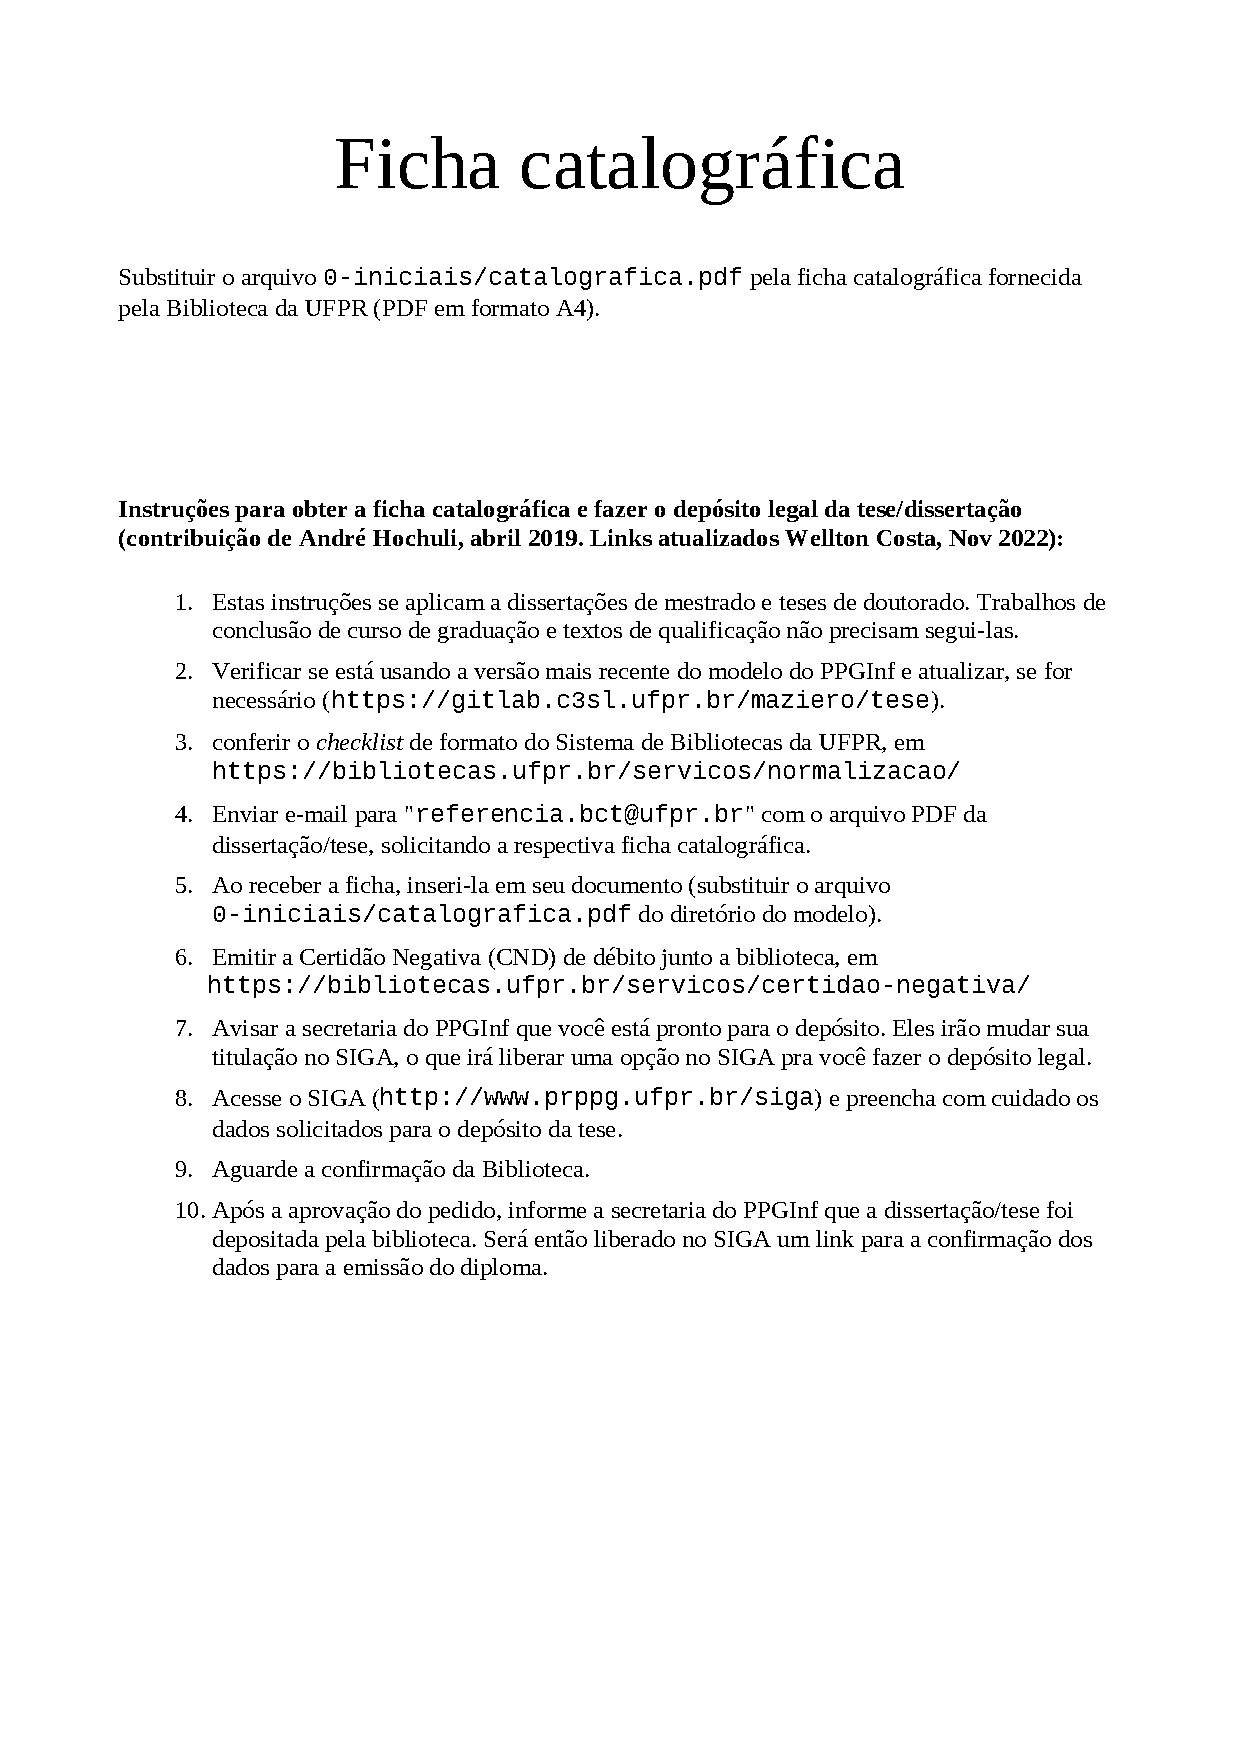
\includepdf[noautoscale]{0-iniciais/catalografica.pdf}

\end{ficha}

%=====================================================
	% ficha catalográfica
% A ficha de aprovação será fornecida pela secretaria do programa,
% após a defesa e cumprimento dos demais trâmites legais.

\begin{aprovacao}	% só gera conteúdo se for na versão final

% inclusão do termo de aprovação final (arquivo PDF)
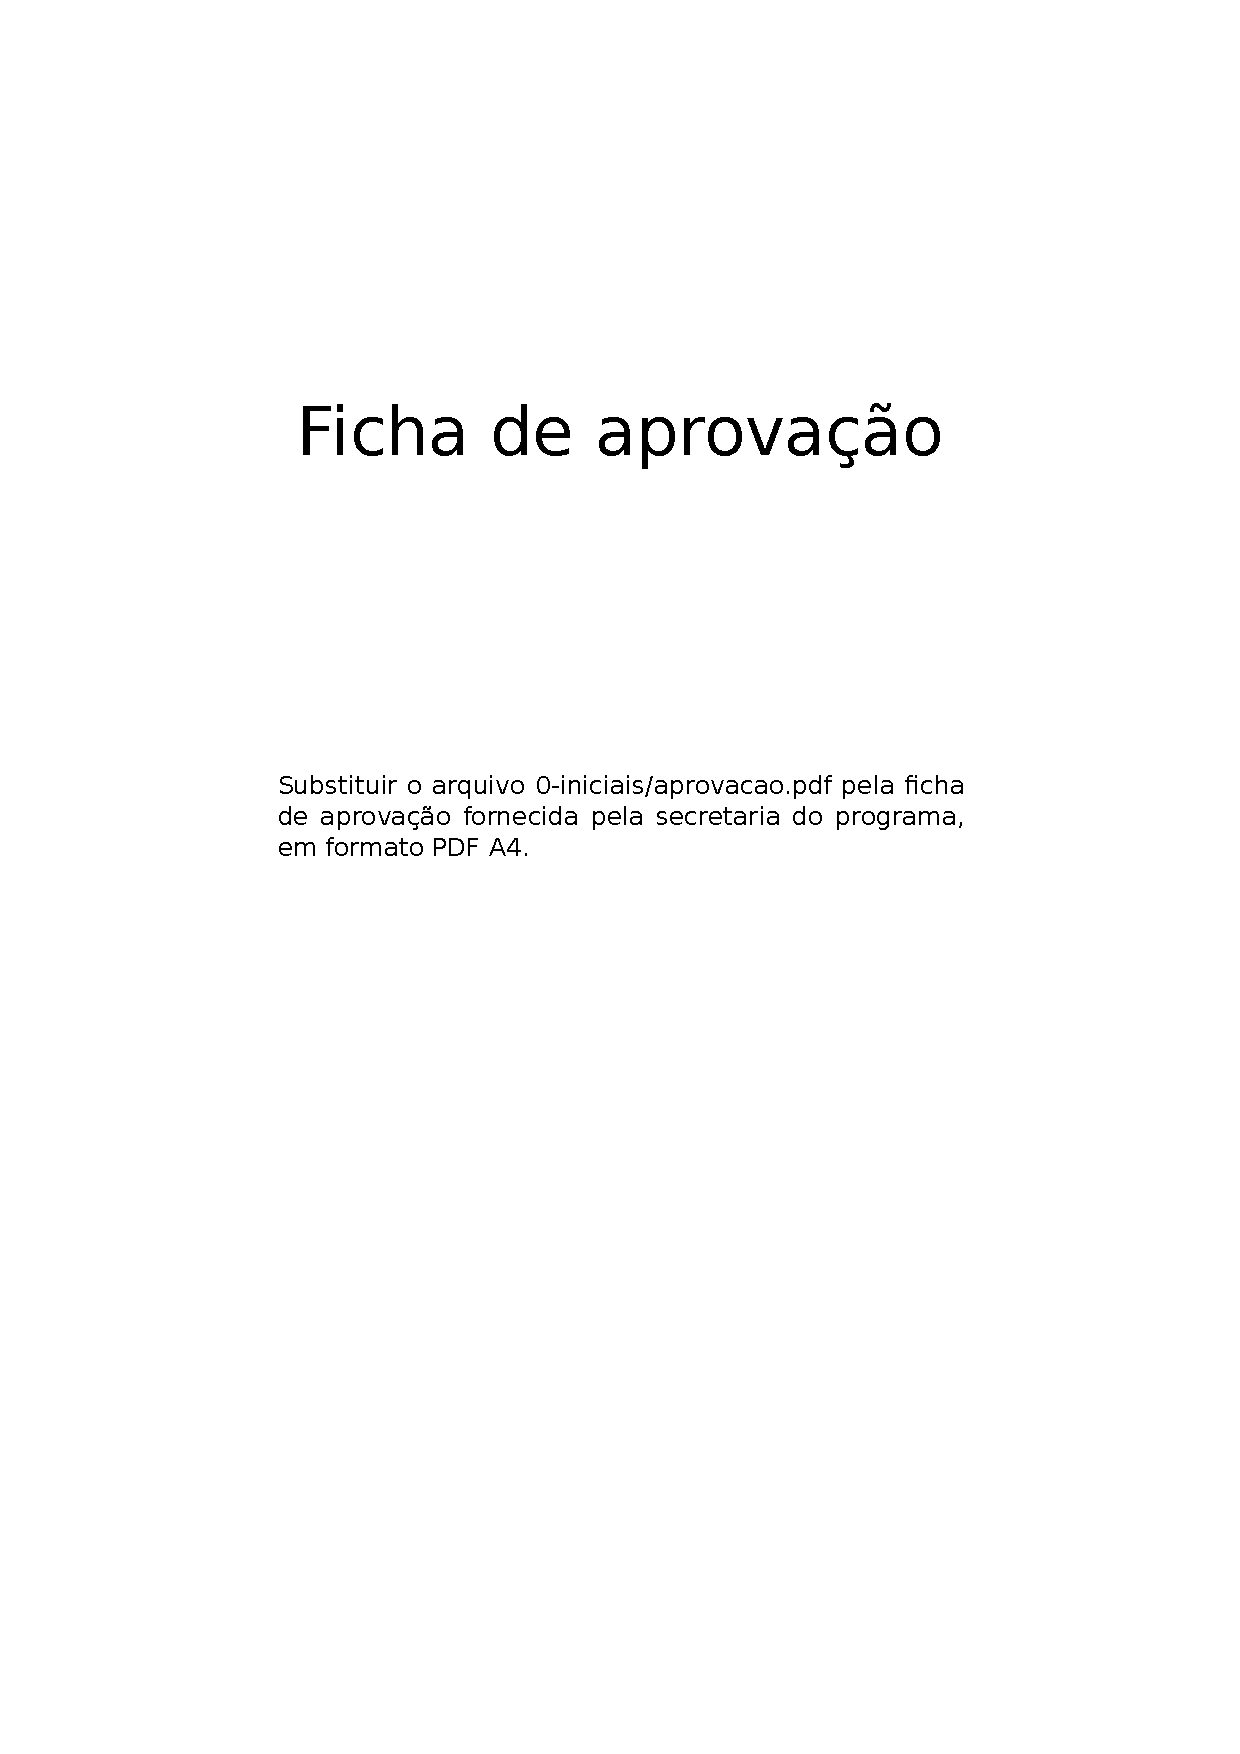
\includepdf[noautoscale]{0-iniciais/aprovacao.pdf}

\end{aprovacao}

%=====================================================
		% folha de aprovação
\begin{dedica}  % só gera conteúdo se for na versão final

A alguém...

\end{dedica}

		% dedicatória
\begin{agradece}	% só gera conteúdo se for na versão final

Inserir os agradecimentos. Os agradecimentos devem ocupar no máximo uma página, devem ser justificados na largura da página e com um afastamento de parágrafo na primeira linha de 1,27 cm. O espaçamento entre linhas deve ser de 1,5 linhas. Não deve haver espaçamento adicional entre parágrafos.

\lipsum[2-5]	% gera um texto aleatório

\end{agradece}

		% agradecimentos

% resumo (português) e abstract (inglês)
\begin{resumo}

Este trabalho explora o problema de encontrar alianças defensivas em grafos, um tema relevante na teoria dos grafos com aplicações em diversas áreas, desde análise de mercado, redes sociais e biologia. Definimos uma aliança defensiva como um subconjunto de vértices onde cada vértice possui pelo menos tantos vizinhos dentro do conjunto quanto fora dele, de forma a ter sempre mais "aliados" do que "inimigos". O texto se concentra na formulação do problema, na análise da complexidade computacional e na implementação de um algoritmo eficiente para a identificação dessas alianças.

Apresentamos um algoritmo FPT semelhante a um busca em profundidade, que explora sistematicamente os vértices do grafo para encontrar alianças defensivas de tamanho específico, juntamente com duas novas melhorias que apresentam melhora significativa no desempenho, e um visualizador web desenvolvido que permite a visualização passo a passo do processo de busca.

\end{resumo}

% \begin{abstract}

The abstract should be the English translation of the ``resumo'', no more, no less.

\lipsum[10-13]	% texto aleatório

\end{abstract}


% listas  de figuras, tabelas, abreviações/siglas, símbolos
% \listoffigures				% figuras
% \clearpage
% \listoftables				% tabelas
% %=====================================================

% lista de acrônimos (siglas e abreviações)

\begin{listaacron}

\begin{longtable}[l]{p{0.2\linewidth}p{0.7\linewidth}}
DINF & Departamento de Informática\\
PPGINF & Programa de Pós-Graduação em Informática\\
UFPR & Universidade Federal do Paraná\\
\end{longtable}

\end{listaacron}

%=====================================================
		% acrônimos, deve ser preenchida à mão
% %=====================================================

% lista de símbolos

\begin{listasimb}

\begin{longtable}[l]{p{0.2\linewidth}p{0.7\linewidth}}
$\alpha$ & alfa, primeira letra do alfabeto grego\\
$\beta$ & beta, segunda letra do alfabeto grego\\
$\gamma$ & gama, terceira letra do alfabeto grego\\
$\omega$ & ômega, última letra do alfabeto grego\\
$\pi$ & pi \\
$\tau$ & Tempo de resposta do sistema\\
$\theta$ & Ângulo de incidência do raio luminoso\\
\end{longtable}

\end{listasimb}

%=====================================================
		% símbolos, idem
\tableofcontents			% sumário

%=====================================================

% define estilo do corpo do documento (capítulos e apêndices)
\mainmatter
\pagestyle{mainmatter}

% inclusao de cada capítulo, alterar a gosto (do professor de Metodologia)
\chapter{Fundamentação teórica}
A fim de seguir de forma devida com a análise do problema e do algoritmo, algumas definições teóricas são requeridas:

\section{Conceitos}

\subsection{Grafo}
Um grafo $G = (V(G), E(G))$ é um par ordenado que consiste de um conjunto de vértices $V(G)$ e um conjunto de arestas $E(G)$.

\subsection{Vértice}
Um vértice $v \in V(G)$ é um elemento básico de um grafo, representando um ponto ou nó na estrutura. O conjunto $V(G)$ é finito e contém todos os vértices do grafo.

\subsection{Aresta}
Uma aresta $e \in E(G)$ é um conjunto de dois vértices de $V(G)$. Em um grafo não direcionado, a aresta $\{u, v\}$ conecta os vértices $u$ e $v$, sem direção. Em grafos direcionados, uma aresta $(u, v)$ conecta $u$ a $v$ com uma orientação de $u$ para $v$.

\subsection{Incidência}
As extremidades de uma aresta são ditas incidentes com a aresta \cite{Bondy2008}, e vice-versa, ou seja, uma aresta $e$ é dita incidente a um vértice $v$ se está aresta se conecta a $v$ em um de seus extremos.

\subsection{Adjacência}
Dois vértices que são incidentes a uma mesma aresta são adjacentes \cite{Bondy2008}, assim como duas arestas que são incidentes a um mesmo vértice, ou seja, um par de vértices distintos $u$ e $v$ são adjacentes se possuem uma aresta que os conectam, da mesma forma que duas arestas distintas $e1$ e $e2$ são adjacentes se são incidentes a um vértice em comum.

\subsection{Vizinhança de um Vértice}
Dois vértices que são incidentes a uma aresta comum, ou seja, dois vértices adjacentes distintos são ditos vizinhos \cite{Bondy2008}. A vizinhança de um vértice $v \in V(G)$, denotada por $N(v)$, é o conjunto de todos os vértices adjacentes a $v$, ou seja, $N(v) = \{ u \in V(G) \mid \{u, v\} \in E(G) \}$ em grafos não direcionados.

\subsection{Grau de um Vértice}
O grau de um vértice $v$ em um grafo não direcionado $G$ é dado por $d(v) = |N(v)|$, ou seja, o número de arestas incidentes a $v$. Neste estudo consideramos apenas grafos não direcionados, portanto o grau de $v$ corresponde ao número de arestas total ligadas a ele.

\subsection{Subgrafo}
Um \textbf{subgrafo} de um grafo $G$ é um grafo $F$ cujos conjuntos de vértices e arestas são subconjuntos dos vértices e arestas de $G$. Formalmente, $F$ é um subgrafo de $G$ se $V(F) \subseteq V(G)$ e $E(F) \subseteq E(G)$, e a função que relaciona vértices e arestas em $F$ é a mesma que em $G$, mas restrita ao conjunto de arestas de $F$. Subgrafos podem ser formados a partir das operações de remoção de vértices e remoção de arestas.\\
Diz-se que $G$ contém $F$ ou que $F$ está contido em $G$, representado como $G \supseteq F$ ou $F \subseteq G$.

\subsection{Conectividade}
Um grafo é \textbf{conexo} se, para toda partição de seu conjunto de vértices em dois conjuntos não vazios $X$ e $Y$, existe uma aresta com uma extremidade em $X$ e a outra extremidade em $Y$, caso contrário, o grafo é desconexo. Em outras palavras, um grafo é desconexo se seu conjunto de vértices pode ser particionado em dois subconjuntos não vazios $X$ e $Y$ de modo que nenhuma aresta tenha uma extremidade em $X$ e outra em $Y$.

\subsection{Aliança Defensiva}
Um subconjunto $S \subseteq V$ é uma aliança defensiva se, para cada vértice $v \in S$, a condição a seguir é satisfeita:   $|N(v) \cap S| \geq |N(v) \setminus S|$.\\
Ou seja, para cada vértice $v$ na aliança $S$, o número de vértices adjacentes a $v$ dentro de $S$ deve ser pelo menos igual ao número de vértices adjacentes a $v$ fora de $S$.\\
Isso indica que os vértices $v$ na aliança devem possuir pelo menos tantos vértices dentro da aliança quanto fora dela.\\
Embora, formalmente, uma aliança não precise ser conexa, note que cada componente conexa de uma aliança é uma aliança por si só. Para fins deste trabalho, toda aliança encontrada deve ser \textbf{conexa}.

\section{Complexidade Computacional}
A complexidade computacional estuda a quantidade de recursos necessários para a execução de algoritmos, especialmente em termos de tempo e espaço. Em ciência da computação, a complexidade computacional é frequentemente representada usando a notação \textit{Big O}, $O(f(n))$, que descreve o crescimento da complexidade como uma função $f(n)$, onde $n$ normalmente é o tamanho da entrada, ou algum outro parâmetro relevante. Alguns exemplos de classificação de complexidade são:

\begin{itemize}
  \item $O(1)$: Constante, o tempo de execução não depende do tamanho da entrada.
  \item $O(n)$: Linear, o tempo de execução cresce proporcionalmente ao tamanho da entrada.
  \item $O(n^k)$: Polinomial, o tempo de execução cresce proporcionalmente com relação a potência $k$ constante do tamanho da entrada. Um exemplo de polinômio muito comum são os quadrados $O(n^2)$.
  \item $O(k^n)$: Exponencial, o tempo de execução cresce de forma exponencial com relação ao tamanho da entrada. No geral, é inviável para grandes entradas.
  \item $O(n!)$ Fatorial, em problemas fatoriais o tempo de execução cresce ainda mais acelerado com relação ao tamanho da entrada do que problemas exponenciais.
\end{itemize}

\subsection{Classes de Complexidade:}
Os problemas de decisão, como os envolvendo alianças, podem ser classificados em certas classes de complexidade que separam o quão viáveis é encontrar ou verificar suas soluções para entradas de larga escala. Estas classes não:

\begin{itemize}
  \item $P$ (Polinomial): Representa a classe de problemas que podem ser resolvidos em tempo polinomial, ou seja, em $O(n^k)$ para algum inteiro $k$. Em ciência da computação, problemas em $P$ são considerados tratáveis.
  \item $NP$ (Tempo polinomial não determinístico): Representa a classe de problemas para os quais, apesar de não sabermos como encontrar solução em tempo polinomial de maneira determinística, dada uma solução, ela pode ser verificada em tempo polinomial por um algoritmo determinístico. Não sabemos se todo problema em $NP$ pode ser resolvido em tempo polinomial, isto é, se $P = NP$, e esse é um dos 7 problemas do milênio que ainda estão em aberto.
  \item $NP$-completo: Representa um subconjunto de problemas em $NP$ que são, intuitivamente, tão difíceis quanto qualquer outro problema em $NP$. Para um problema ser dessa classe, são necessárias duas características:
  \begin{enumerate}
    \item Estar em $NP$, ou seja, dada uma solução, ela deve ser verificável em tempo polinomial.
    \item Ser $NP$-difícil, todo problema em $NP$ pode ser redutível a ele em tempo polinomial.\\
Em outras palavras, caso um problema de classe $NP$-completo seja resolvido em tempo polinomial, todos os outros problemas em $NP$ poderão ser resolvidos em tempo polinomial.
  \end{enumerate}
\end{itemize}

\section{O algoritmo}
Como encontrar uma aliança defensiva em um grafo é um problema NP-completo, o algoritmo FPT \cite{Enciso2009} tem como objetivo buscar por uma aliança conexa arbitrária de tamanho máximo $k$, a fim de tornar o problema tratável. Porém, neste trabalho o tamanho da aliança buscada será \textit{exatamente} $k$, pois acreditamos que o tamanho da aliança seja importante. Antes de entrar na explicação minuciosa do algoritmo, é importante explicar o que é um algoritmo FPT.

\subsection{Complexidade}
FPT (\textit{Fixed-Parameter Tractable}) é uma classe de complexidade que trata de problemas parametrizáveis (como os de complexidade exponencial) ao isolar e fixar um parâmetro específico do problema, chamado $k$, e então expressando a complexidade na forma $f(k)*p(n).$ Desta forma, $f(k)$ é a parte da complexidade que depende exclusivamente de $k$ e pode ser \textit{superpolinomial}, enquanto $p(n)$ é uma função polinomial de $n$. Sendo assim, fixar $k$ em valores pequenos nos permite abordar o algoritmo de forma mais tratável, custando muito menos tempo, a depender do tamanho de $k$.

O algoritmo usado neste estudo foi proposto por \cite{Enciso2009}, e tem complexidade $O(k^kn)$, e é uma melhora significativa de seu predecessor, que tinha complexidade $O((2k-1)^kk^2n)$. Esse é um avanço substancial, mas ainda é interessante demonstrar como problemas, mesmo parametrizados, crescem rapidamente:

\begin{table}[h]
\begin{center}
\begin{tabular}{|c|c|c|c|c|c|c|c|}
\hline
$k$ & $k^k$\\
\hline
2 & 4 \\
\hline
3 & 27 \\
\hline
4 & 256 \\
\hline
5 & 3.125 \\
\hline
6 & 46.656 \\
\hline
7 & 823.543 \\
\hline
9 & 387.420.489 \\
\hline
10 & 10.000.000.000 \\
\hline
\end{tabular}
\end{center}
\end{table}

\begin{figure}[!htb]
\centering
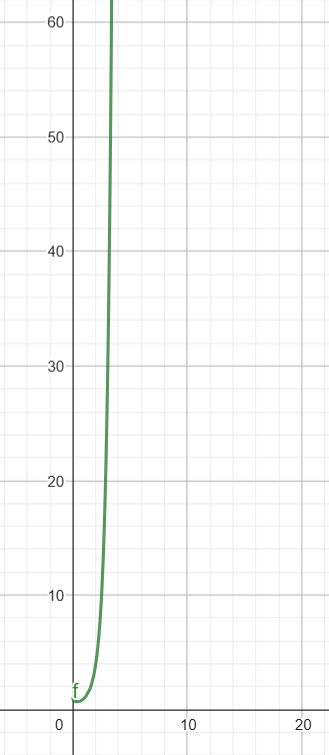
\includegraphics[height=12cm]{GraficoKelevK.png}
\caption{Gráfico da função $k^k$}
\label{fig:kelevk}
\end{figure}

O propósito do algoritmo então é garantir que o tempo possa ser diminuído de acordo com $k$, sem que seja necessário executar para todo $n-k$ restante.

\subsection{Explicação}
O algoritmo é dividido em duas funções principais, a \texttt{main} e a \texttt{defensiveAlliance}. A \texttt{main} recebe como entrada um Grafo $G$ e o tamanho da aliança desejada, um inteiro positivo $k$. De forma intuitiva, a abordagem do algoritmo é partir de um vértice do grafo por vez e olhar sua vizinhança numa tentativa de expandi-lo até formar uma aliança defensiva de tamanho $k$, ou todos os vértices terem servido de raiz da expansão.

\lstset{ 
  deletekeywords={do}  
}

\begin{lstlisting}[escapeinside={(*}{*)}]
Main(G,k)
	Para cada vértice v de G:
		v.c_w <- (*$\ceil{\frac{d(v)}{2}}$*).
	Para cada vértice v de G:
		inicia uma aliança S <- {v}.
		aliança_encontrada <- DefensiveAlliance(S).
		Se aliança_encontrada:
			retorne aliança_encontrada.
		retira v de S
		soma 1 ao c_w de v.
			
	retorne "Sem aliança";
\end{lstlisting}

O papel da função \texttt{main} é garantir que todos os vértices foram usados como raiz da expansão. Para isso, primeiro é definido o \texttt{c\_w}, que serve para verificar se o vértice está protegido dentro da aliança \texttt{S}. De início, ela é definida com o número de vizinhos necessários dentro de $S$ para que ele esteja defendido, e então será aumentada ou diminuida conforme se adiciona ou remove seus vizinhos a $S$.

Isso também faz parte da condição de sucesso da busca, ou seja, quando todos os vértices de \texttt{S} estiverem protegidos (\texttt{c\_w <= 0}) então uma aliança defensiva foi formada.

A seguir, a \texttt{main} chama a função \texttt{defensiveAlliance} para verificar se \texttt{S} é, ou pode ser expandida até, uma aliança defensiva de tamanho \texttt{k}.

\begin{lstlisting}[escapeinside={(*}{*)}]
DefensiveAlliance(G, S, k)
	inicia v <- vértice de maior c_w em S.
	Se v.c_w <= 0 e tamanho de S == k:
		devolve S.
		
	Se v.c_w <= k - tamanho de S: 
		inicia t <- 1 + metade dos vizinhos de w.
		inicia o conjunto W <- t vizinhos de w que não pertencem a S.
		Para cada vértice w em W:
			S <- S + w.
			Para cada vizinho x de w em S:
				subtrai 1 do c_w de x e de w.
			aliança_encontrada <- DefensiveAlliance(G, S, k)
			Se aliança_encontrada:
				Devolve aliança_encontrada.
			Para cada vizinho x de w em S:
				soma 1 ao c_w de x e de w.
			Retira w de S.
			
	Retorne NULL;
\end{lstlisting}

No início de \texttt{defensiveAlliance} o algoritmo escolhe o vértice de maior \texttt{c\_w} em \texttt{S},  que seria o vértice mais vulnerável da aliança. Esse vértice serve para tanto verificar se \texttt{S} se tornou uma aliança quanto como ponto de expansão a fim de incluir novos vértices.

A seguir, o algoritmo verifica se há espaço em \texttt{S} para os \texttt{c\_w} vizinhos necessários serem adicionados, ou seja, para que \texttt{w} seja defendido dentro da restrição do tamanho máximo \texttt{k}. Essa verificação funciona de modo semelhante a uma heurística de busca, poupando tempo ao evitar vértices que não podem ser defendidos posteriormente.

\subsection{Lema 14}
Uma parte importante do funcionamento do algoritmo é o lema 14 de \cite{Enciso2009}. Assuma que $S \subseteq V$ é estendível para uma aliança defensiva S', onde $|S| <|S'| = k$ então, para qualquer vértice desprotegido $w \in S$, $|S' \cap (N[w] - S|) \ge c_w$.\\
Em outras palavras se $S$ é estendível e $w$ é um vértice desprotegido de $S$ então $c_w$ é o número de vizinhos de $w$ fora de $S$ que é necessário para proteger $w$ em $S$.

Esse lema é o que podemos considerar como o núcleo do algoritmo, pois ele nos garante também que para qualquer subconjunto $W \subseteq N[w] - S$ com $t = \lfloor \frac{d_w}{2} \rfloor + 1$  vértices contém ao menos um vértice $w_i$ para o qual $S \cup {w_i}$ é estendível se e somente se S é estendível.

\subsection{Evitando repetir conjuntos}
Observando o comportamento do algoritmo no visualizador web foi possível notar que um comportamento pouco eficiente: o critério de expansão de $S$ (destacado a seguir) abre margem pra repetir várias vezes a mesma combinação de vértices, levando, principalmente em grafos de grande quantidade de vértices, a muito esforço improdutivo.

\begin{lstlisting}
DefensiveAlliance(G, S, k)
	inicia v <- vértice de maior c_w em S.
\end{lstlisting}

Pensando nisso a equipe elaborou uma solução que armazena todas as combinações já analisadas anteriormente e impede de que novas iterações com elas sejam geradas, cortando toda a sub-árvore subsequente. Isso é feito com a criação de um dicionário e a marcação única de cada combinação:

\begin{lstlisting}
inicia combinacoes <- dicionário vazio
\end{lstlisting}

\begin{lstlisting}
DefensiveAlliance(G, S, k)
[...]
	Para cada vértice w em W:
		S <- S + w.
		
		comb_id <- identificadores de S de forma ordenada.
		Se existe combinacoes[comb_id]:
			Retira w de S.
			pula para o próximo vértice.
		Caso contrário:	
			cria combinacoes[comb_id].

		Para cada vizinho x de w em S:
			subtrai 1 do c_w de x e de w.
		aliança_encontrada <- DefensiveAlliance(G, S, k)
[...]
\end{lstlisting}

Caso não exista uma entrada da combinação no dicionário, cria-se uma e a instância corrente de \texttt{S} é analisada. Caso contrário, a instância é ignorada, podando todas as sub-árvores subsequentes. A complexidade de tempo é se resume a ordenação de, no máximo, $k-1$ elementos, e ao acesso e escrita no dicionário. Ambos são ofuscados pela complexidade geral.

Por outro lado, há um custo sério em termos de espaço. No pior caso, de não haver aliança e o algoritmo analisar todos os vértices e $k=n$, a combinação ocupa espaço $O(2^n)$, que corresponde a guardar todas as combinações de $n$ vértices, variando de tamanho $1$ até $n$. Isso pode ser mitigado ao limitar o tamanho das combinações armazenadas para a região crítica que vai ser repetida mais vezes. A análise desta região está na seção sobre Resultados e discussão.

Quanto ao desempenho, esta técnica permite ao algoritmo poupar muito tempo ao "amortizar" o custo $k^k$ ao longo de várias iterações, pois, como nenhuma combinação é repetida, quanto mais exploradas são as combinações dos vértices, menos combinações existem para serem analisadas.

\subsection{Priorização dos vértices expostos}
\begin{lstlisting}
DefensiveAlliance(G, S, k)
	inicia v <- vértice de maior c_w em S.
\end{lstlisting}

Ao iniciarmos $DefensiveAlliance(G,S,k)$ atribuindo $v$ o vértice em $W$ com maior $c_w$ nós garantimos que a maior prioridade em cada chamada recursiva da função é proteger o vértice mais "exposto".

Assim obtemos também um critério de parada consistente, ou seja, quando o vértice com maior $c_w$ ter $c_w \le 0$ e $|S| = k$, teremos duas informações fundamentais sobre o contexto da execução:\\
1 - Se $c_w \le 0$, então todos os vértices em $S$ estão protegidos.\\
2 - Se $|S|=k$, encontramos a aliança defensiva procurada.

\chapter{Metodologia}
O projeto é composto por duas partes principais: algoritmos de busca implementados em Python e um visualizador web criado para exibir os passos deste algoritmo. As partes funcionam de forma independente, sendo conectadas apenas pelo formato de entrada e saída dos programas.

\section{Algoritmo em Python}
A implementação do algoritmo proposto por \cite{Enciso2009} foi feita em Python e consta completa no Apêndice 1.

Nesta implementação foi utilizada a estrutura de dados da biblioteca \textit{Networkx} para manipulação dos grafos, e, no mais, estruturada de forma semelhante ao algoritmo teórico, com a exceção do uso de uma estrutura de pilha para substituir a chamada recursiva.

Além do resultado final, o programa possibilita o retorno da aliança em formato JSON, com as características utilizadas no visualizador web. Essas características permitem a visualização passo a passo dos nós expandidos pelo algoritmo, e consistem do conjunto $W$ a cada iteração da função \texttt{DefensiveAlliance}.

Há também \textit{flags} para mostrar a quantidade de nós expandidos, para gerar um grafo aleatório segundo uma densidade especificada, e para alterar o comportamento da busca, como retornar a primeira aliança encontrada independente do tamanho.

\section{Visualizador web}
O projeto web foi desenvolvido com Typescript e React, e sua proposta é fornecer uma visualização passo-a-passo do algoritmo e do grafo de entrada. Assim como o algoritmo de busca, o visualizador pode ser encontrado no repositório que se encontra nas referências.

Para montar a visualização é necessário que seja fornecido como entrada um grafo disposto em formato JSON, contando com dois conjuntos extras de dados que são a aliança encontrada, caso exista, e um vetor de \textit{steps}, que contém o conjunto $W$ no dado \textit{passo} da iteração.

Munido destas informações, o visualizador organiza os dados internamente para melhorar o desempenho e a decisão de cada caraterística visual do grafo e então personaliza uma \textit{view} HTML, dada pela biblioteca 3d-force-graph \cite{HassanShafique2004}, que cuida da renderização e simulação física do grafo.

Dentre as funcionalidades, vale destacar duas principais: a visualização do conjunto $S$ a cada etapa do algoritmo e o mapa de calor dos nós explorados. O mapa de calor é a coloração dos vértices do grafo seguindo a regra de que, quanto mais visitado um vértice durante a execução do algoritmo, mais quente é a cor usada; os nós mais quentes tem cores próximas do vermelho, e os mais frios, mais próximas do azul.

\subsection{Visualização por passos}
Ao carregar um grafo com o conjunto de passos, é possível navegar por cada um deles. Em um certo passo, os vértices e arestas da fronteira de $S$ são desenhados com uma cor cinza escura, os além da fronteira tem cor cinza claro, e os vértices dentro de $S$ ficam coloridos com a cor

\begin{itemize}
  \item azul, se estiverem desprotegidos;
  \item ou verde, se estiverem devidamente protegidos.
\end{itemize}

Ao finalizar o algoritmo e desenhar a aliança, ela é colorida de verde escuro.

As figuras a seguir são de uma busca por uma aliança de tamanho $k = 15$ em um grafo de $v=50$ vértices e $e=40$ arestas. O algoritmo começa com $S$ contendo o vértice colorido de azul.

\begin{figure}[!htb]
\centering
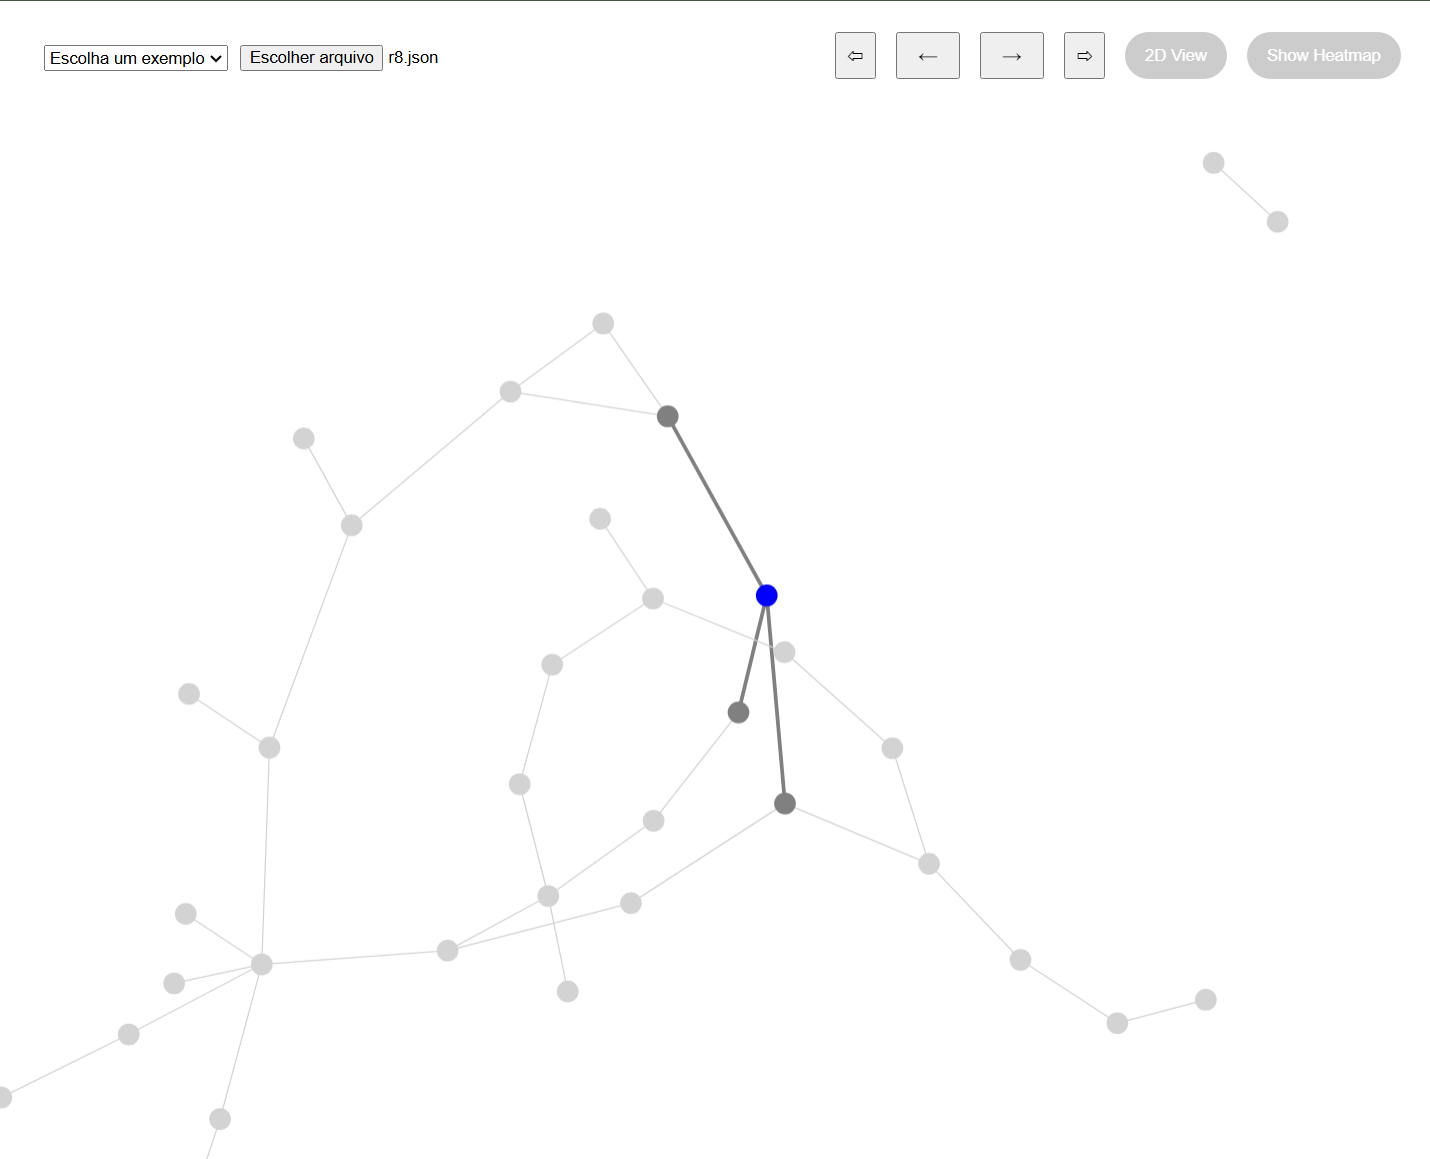
\includegraphics[width=12cm]{GrafoSteps1.png}
\caption{Passo 1 do algoritmo}
\label{fig:grafo-steps-1}
\end{figure}

\begin{figure}[!htb]
\centering
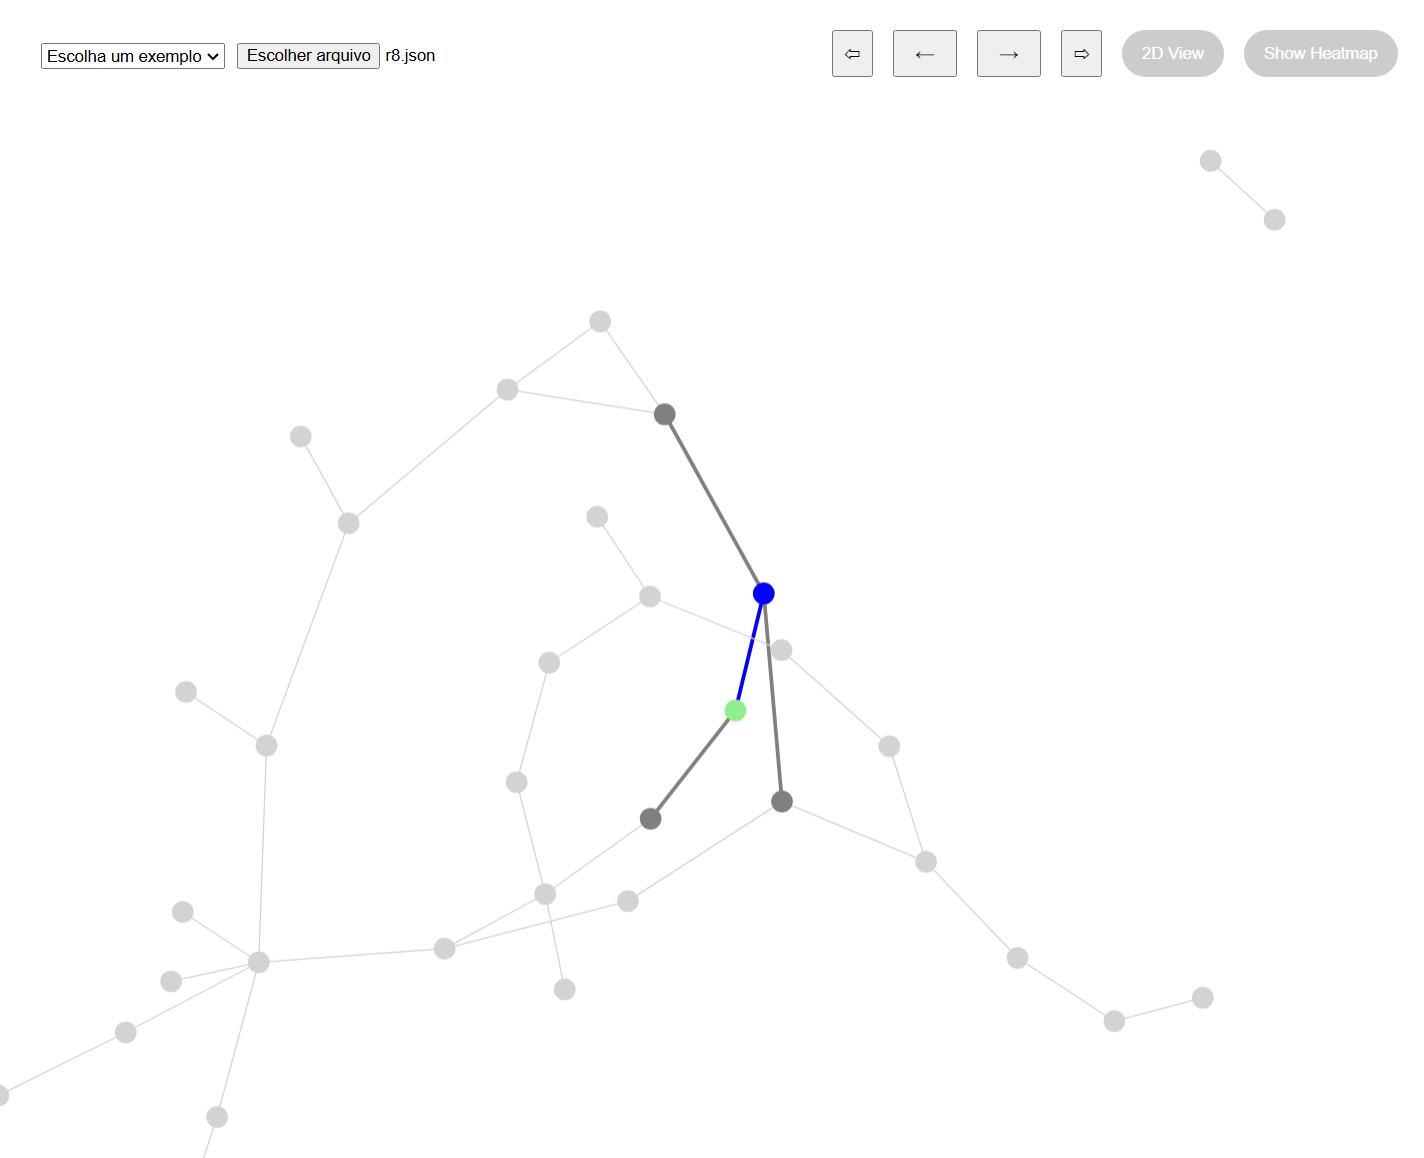
\includegraphics[width=12cm]{GrafoSteps2.png}
\caption{Passo 2 do algoritmo}
\label{fig:grafo-steps-2}
\end{figure}

\begin{figure}[!htb]
\centering
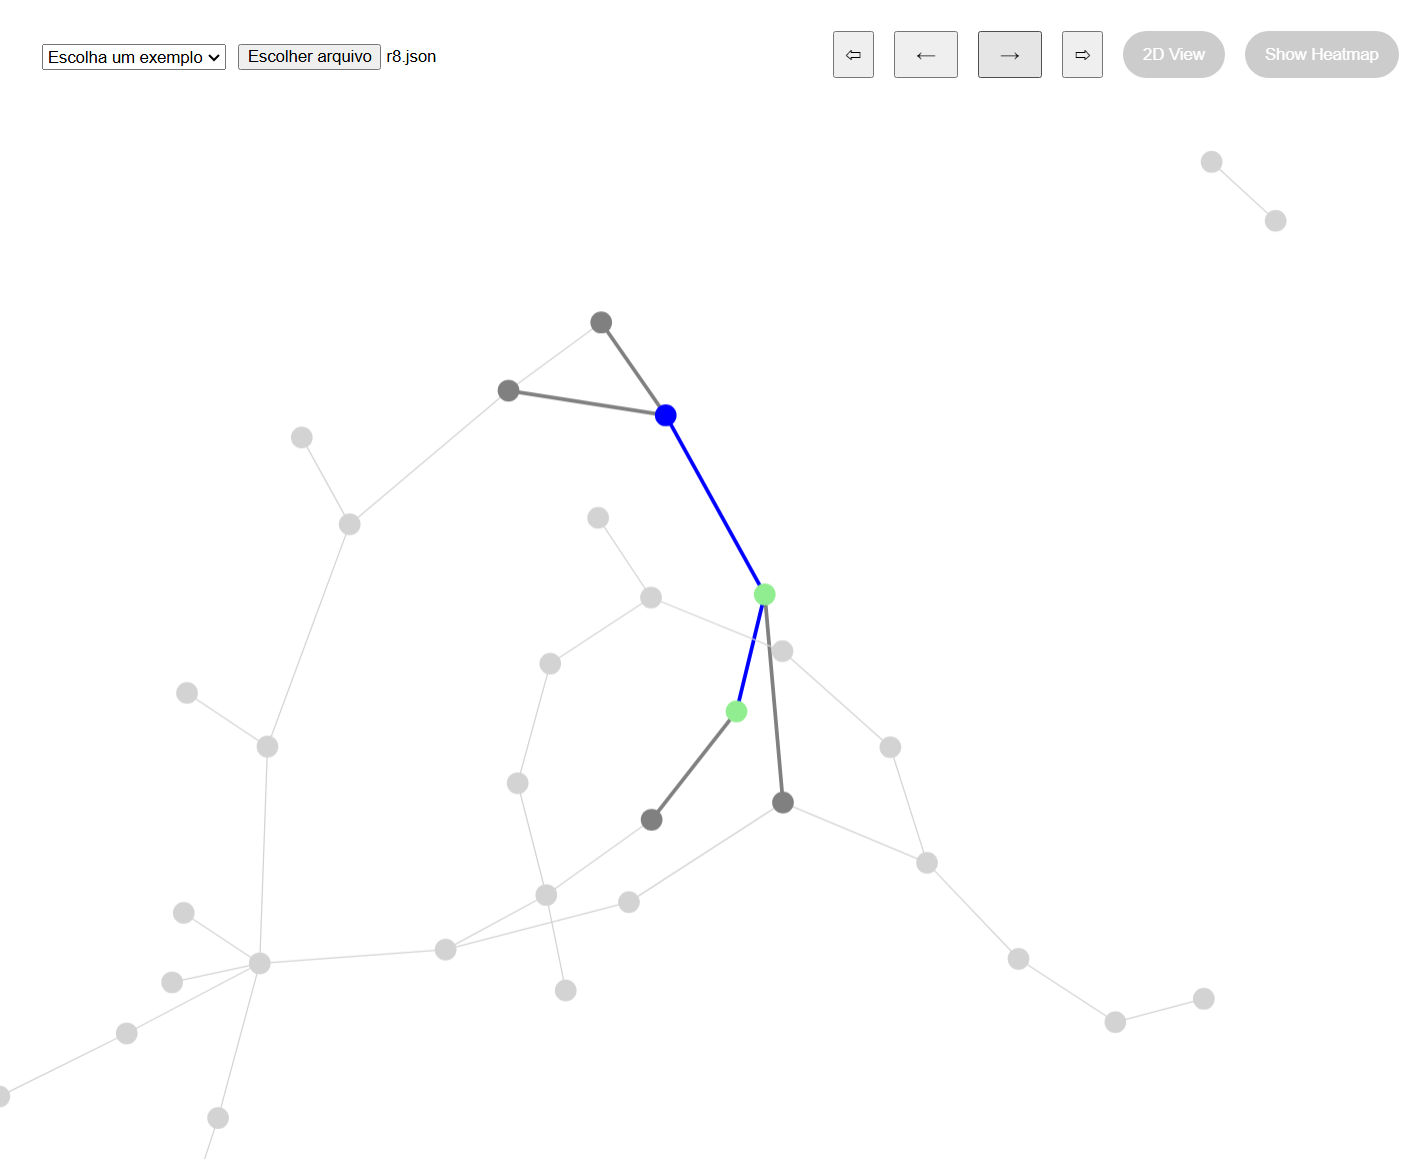
\includegraphics[width=12cm]{GrafoSteps3.png}
\caption{Passo 3 do algoritmo}
\label{fig:grafo-steps-3}
\end{figure}

\begin{figure}[!htb]
\centering
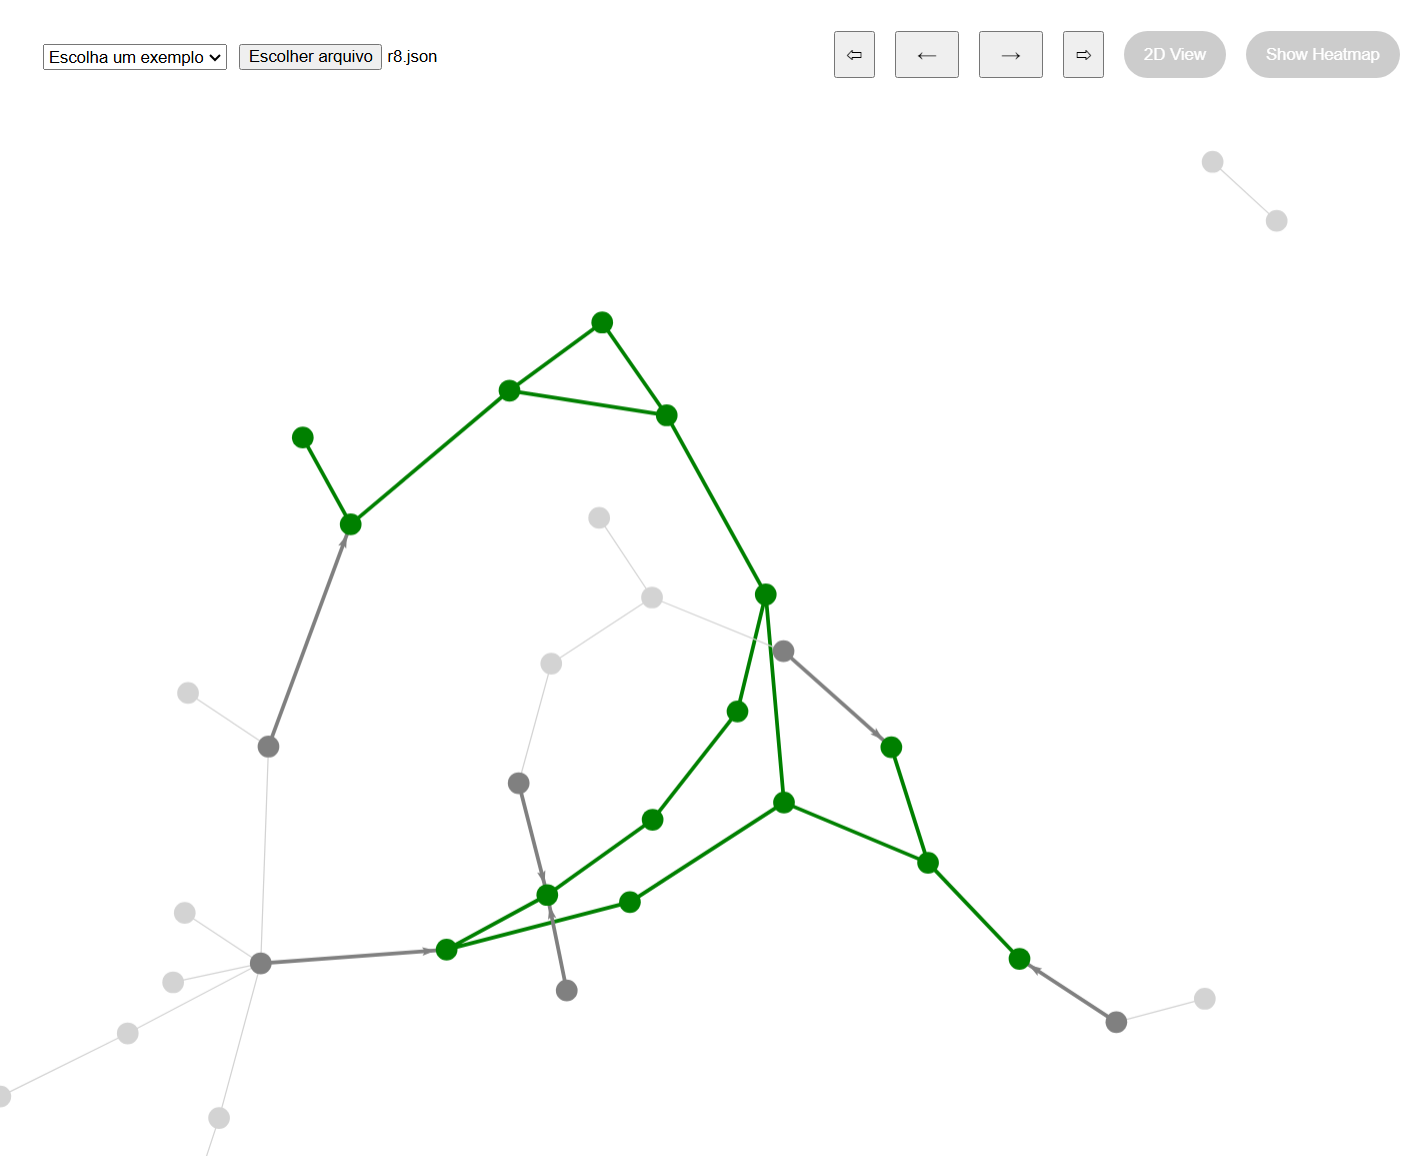
\includegraphics[width=12cm]{GrafoStepsN.png}
\caption{Passo final do algoritmo}
\label{fig:grafo-steps-n}
\end{figure}

\subsection{Mapa de calor}
É possível também ativar a visualização do mapa de calor, que colore os vértices de acordo com a quantidade de vezes que ele foi explorado pelo algoritmo.

\begin{figure}[!htb]
\centering
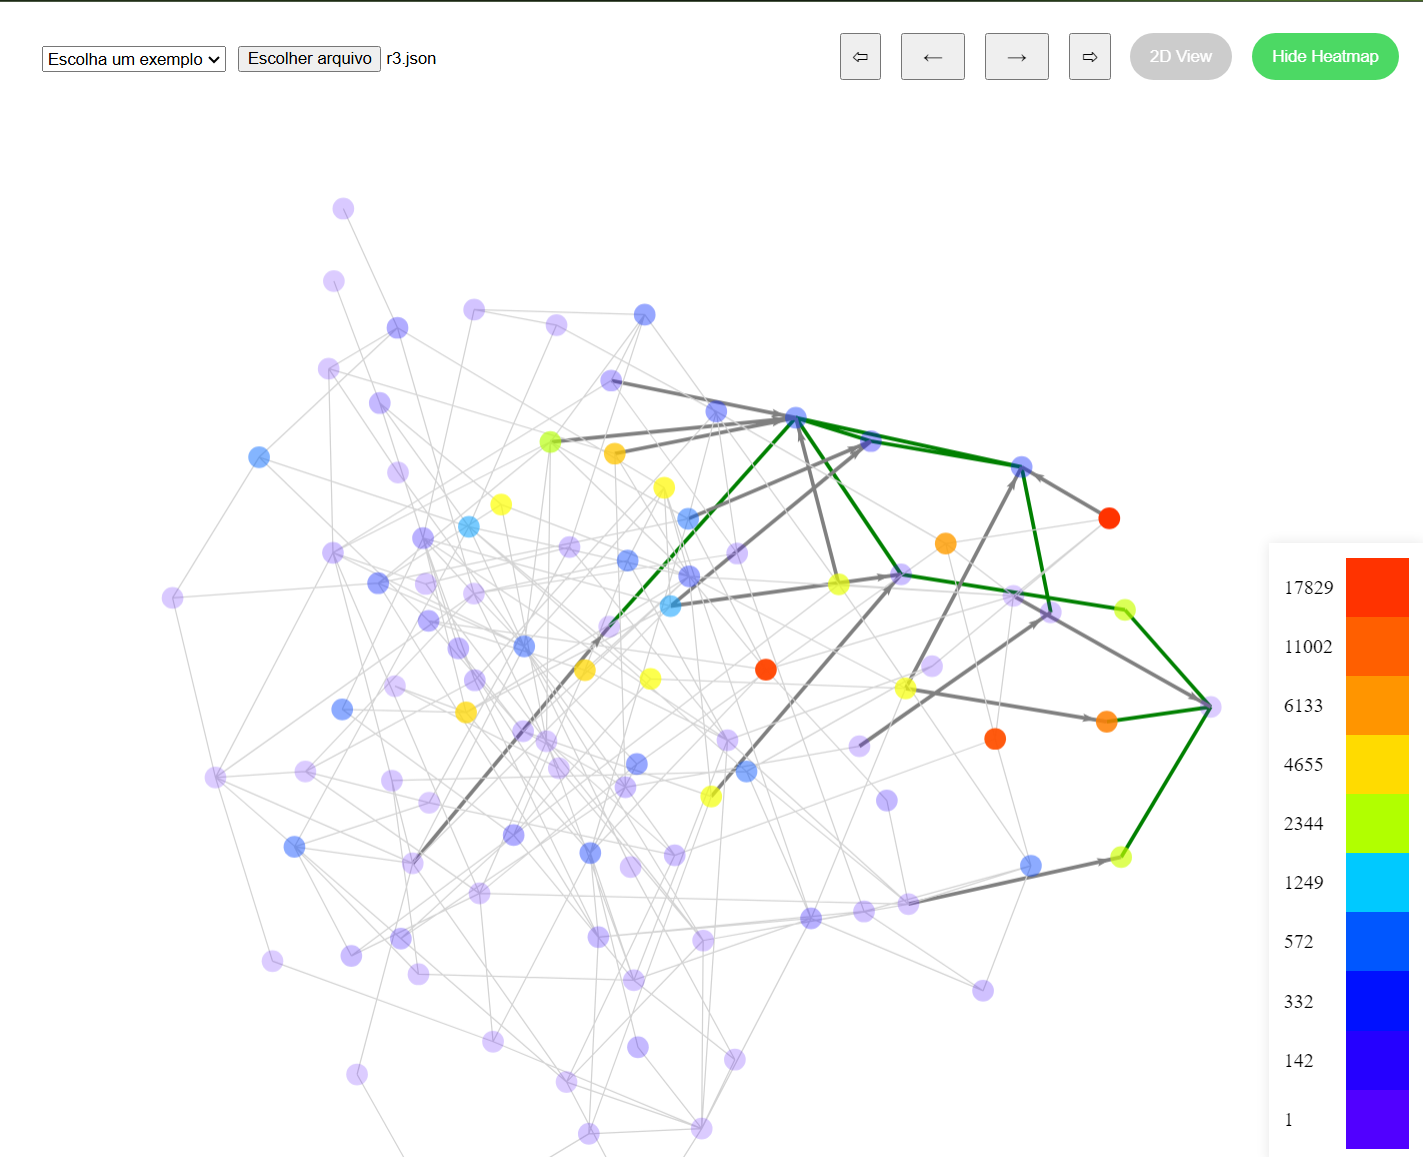
\includegraphics[width=12cm]{GrafoHeatmap.png}
\caption{Mapa de calor do grafo}
\label{fig:grafo-heatmap}
\end{figure}

Para ajudar na visualização, as cores mais frias também tem opacidade mais baixa.

Essa ferramenta em particular incentivou questionamentos interessantes a respeito da eficiência do algoritmo, como "como evitar a alta taxa de repetição de um grupo de vértices".

\chapter{Resultados e discussão}
O algoritmo originalmente estudado e a versão com as melhorias propostas foram analisadas e submetidas a um conjunto de testes para melhor ilustrar o impacto e eficiência de cada uma. Visto que o problema continua sendo NP-completo, há pouco a ser feito para valores realmente grandes, mas foi possível sim observar uma ampliação dos valores considerados "razoáveis" pelo algoritmo FPT.

Para testar o algoritmo utilizamos a função da biblioteca \texttt{networkx nx.erdos\_renyi\_graph(v,e,seed)} onde \texttt{v} é o número de vértices \texttt{e} é a probabilidade de 2 vértices formarem uma aresta, e \texttt{seed} é uma semente para geração do Grafo.

Para os testes a seguir foram fixados os seguintes seguintes parâmetros \texttt{v=30} \texttt{e=0.333} e \texttt{seed=100} e executamos para \texttt{k} variando entre \texttt{1} e \texttt{29}.

\begin{figure}[!htb]
\centering
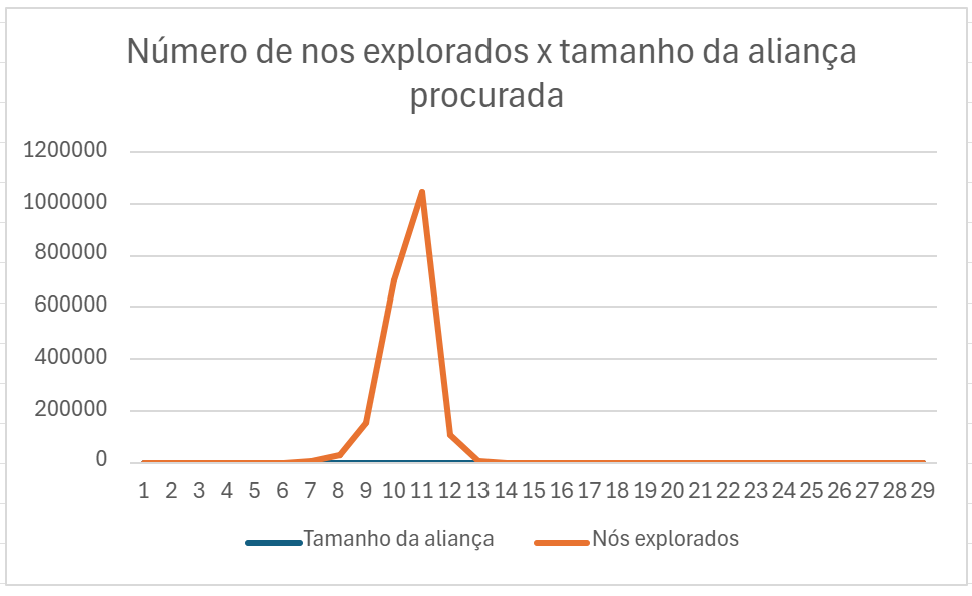
\includegraphics[width=12cm]{Execução sem repetição de conjuntos.png}
\caption{Execução do algoritmo \textbf{evitando} a repetição de conjuntos}
\label{fig:execucao-sem-repeticao}
\end{figure}

Na execução do algoritmo sem repetição de conjuntos é possível notar que o número máximo de nós explorados foi de aproximadamente 1 milhão de nós.

\begin{figure}[!htb]
\centering
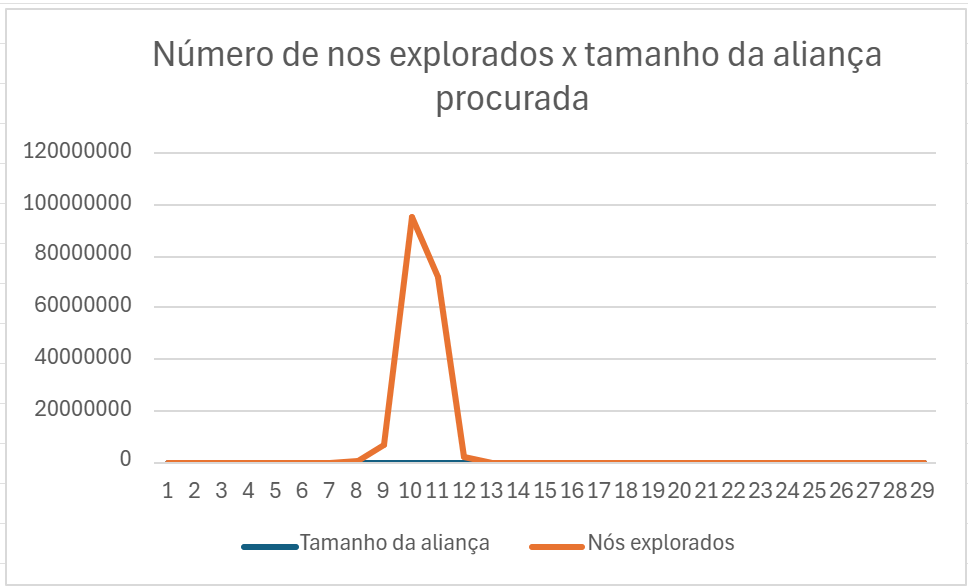
\includegraphics[width=12cm]{Execução com repetição de conjuntos.png}
\caption{Execução do algoritmo \textbf{permitindo} a repetição de conjuntos}
\label{fig:execucao-com-repeticao}
\end{figure}

Por sua vez, na execução que permite a repetição de conjuntos o número de nós explorados nesse caso saltou de 1 milhão para 100 milhões.

Salvar os conjuntos resulta em uma melhora significativa na redução do número de nós a serem explorados, porém nós traz um novo problema pois o espaço necessário para armazenar todos esses conjuntos no pior caso é $\sum_{i=0}^{k} \binom{n}{i}<2^n$, ou seja, acabamos trocando um tempo exponencial, por espaço exponencial.

Foi observado um padrão interessante na eficiência com relação ao grau médio dos vértices do grafo $d(G)$ e $k$; o número de nós explorados atinge um ápice para valores de $k$ próximos de $d(G)$ criando uma "zona difícil", e suaviza a medida que a diferença aumenta.

Para valores de $d(G)$ muito maiores que $k$ isso acontece porque o algoritmo pode descartar muitas combinações através do critério \texttt{Se v.c\_w <= k - tamanho de S:}. Essa linha garante que o próximo nó a ser expandido ao menos tem as condições de ser protegido dado o tamanho atual de $S$.

Por outro lado, valores de $k$ muito menores do que $d(G)$, foi observado uma probabilidade maior de haver uma aliança defensiva. A modificação de ordenação dos vértices de \texttt{W} com base em quantos vizinhos ele possui em $S$ e $\lfloor d(v)/2 \rfloor$, em especial, mostrou acelerar muito o processo de determinação da aliança, quando existente. Isso se deve as escolhas priorizarem a defesa dos vértices já em $S$, em prol de adições aleatórias.

Por fim, a modificação de "Evitar repetir conjuntos" mostrou-se acelerar o processo tanto no melhor caso quanto no pior, pois garante que somente novas combinações são testadas.

\chapter{Conclusão}
O estudo como um todo foi bastante produtivo dentro do tema, e possibilitou compreensão significativa do que são e como encontrar alianças defensivas. O visualizador web, como ferramenta didática, foi bastante aproveitado para a compreensão e elaboração das melhorias propostas ao algoritmo.

Também foi produtivo experimentar na prática a complexidade de um problema NP-completo e uma das ferramentas usadas para contornar esse degrau gigantesco na complexidade.

Dentre os diversos temas que podem ser abordados em discussões futuras, destacamos a implementação e análise do algoritmo proposto por \cite{Enciso2009} para encontrar Conjuntos Seguros (\textit{Secure Sets}), que segue uma abordagem FPT semelhante ao de alianças defensivas, e pode ser adaptado para o visualizador web para gerar resultados valiosos.

Outro ponto de possível expansão é o de pré-análise de grafos para a determinação de potencial de uma aliança de tamanho $k$, partindo da análise feita sobre o grau médio e a "zona difícil".
			% introdução
\chapter{Fundamentação teórica}
A fim de seguir de forma devida com a análise do problema e do algoritmo, algumas definições teóricas são requeridas:

\section{Conceitos}

\subsection{Grafo}
Um grafo $G = (V(G), E(G))$ é um par ordenado que consiste de um conjunto de vértices $V(G)$ e um conjunto de arestas $E(G)$.

\subsection{Vértice}
Um vértice $v \in V(G)$ é um elemento básico de um grafo, representando um ponto ou nó na estrutura. O conjunto $V(G)$ é finito e contém todos os vértices do grafo.

\subsection{Aresta}
Uma aresta $e \in E(G)$ é um conjunto de dois vértices de $V(G)$. Em um grafo não direcionado, a aresta $\{u, v\}$ conecta os vértices $u$ e $v$, sem direção. Em grafos direcionados, uma aresta $(u, v)$ conecta $u$ a $v$ com uma orientação de $u$ para $v$.

\subsection{Incidência}
As extremidades de uma aresta são ditas incidentes com a aresta \cite{Bondy2008}, e vice-versa, ou seja, uma aresta $e$ é dita incidente a um vértice $v$ se está aresta se conecta a $v$ em um de seus extremos.

\subsection{Adjacência}
Dois vértices que são incidentes a uma mesma aresta são adjacentes \cite{Bondy2008}, assim como duas arestas que são incidentes a um mesmo vértice, ou seja, um par de vértices distintos $u$ e $v$ são adjacentes se possuem uma aresta que os conectam, da mesma forma que duas arestas distintas $e1$ e $e2$ são adjacentes se são incidentes a um vértice em comum.

\subsection{Vizinhança de um Vértice}
Dois vértices que são incidentes a uma aresta comum, ou seja, dois vértices adjacentes distintos são ditos vizinhos \cite{Bondy2008}. A vizinhança de um vértice $v \in V(G)$, denotada por $N(v)$, é o conjunto de todos os vértices adjacentes a $v$, ou seja, $N(v) = \{ u \in V(G) \mid \{u, v\} \in E(G) \}$ em grafos não direcionados.

\subsection{Grau de um Vértice}
O grau de um vértice $v$ em um grafo não direcionado $G$ é dado por $d(v) = |N(v)|$, ou seja, o número de arestas incidentes a $v$. Neste estudo consideramos apenas grafos não direcionados, portanto o grau de $v$ corresponde ao número de arestas total ligadas a ele.

\subsection{Subgrafo}
Um \textbf{subgrafo} de um grafo $G$ é um grafo $F$ cujos conjuntos de vértices e arestas são subconjuntos dos vértices e arestas de $G$. Formalmente, $F$ é um subgrafo de $G$ se $V(F) \subseteq V(G)$ e $E(F) \subseteq E(G)$, e a função que relaciona vértices e arestas em $F$ é a mesma que em $G$, mas restrita ao conjunto de arestas de $F$. Subgrafos podem ser formados a partir das operações de remoção de vértices e remoção de arestas.\\
Diz-se que $G$ contém $F$ ou que $F$ está contido em $G$, representado como $G \supseteq F$ ou $F \subseteq G$.

\subsection{Conectividade}
Um grafo é \textbf{conexo} se, para toda partição de seu conjunto de vértices em dois conjuntos não vazios $X$ e $Y$, existe uma aresta com uma extremidade em $X$ e a outra extremidade em $Y$, caso contrário, o grafo é desconexo. Em outras palavras, um grafo é desconexo se seu conjunto de vértices pode ser particionado em dois subconjuntos não vazios $X$ e $Y$ de modo que nenhuma aresta tenha uma extremidade em $X$ e outra em $Y$.

\subsection{Aliança Defensiva}
Um subconjunto $S \subseteq V$ é uma aliança defensiva se, para cada vértice $v \in S$, a condição a seguir é satisfeita:   $|N(v) \cap S| \geq |N(v) \setminus S|$.\\
Ou seja, para cada vértice $v$ na aliança $S$, o número de vértices adjacentes a $v$ dentro de $S$ deve ser pelo menos igual ao número de vértices adjacentes a $v$ fora de $S$.\\
Isso indica que os vértices $v$ na aliança devem possuir pelo menos tantos vértices dentro da aliança quanto fora dela.\\
Embora, formalmente, uma aliança não precise ser conexa, note que cada componente conexa de uma aliança é uma aliança por si só. Para fins deste trabalho, toda aliança encontrada deve ser \textbf{conexa}.

\section{Complexidade Computacional}
A complexidade computacional estuda a quantidade de recursos necessários para a execução de algoritmos, especialmente em termos de tempo e espaço. Em ciência da computação, a complexidade computacional é frequentemente representada usando a notação \textit{Big O}, $O(f(n))$, que descreve o crescimento da complexidade como uma função $f(n)$, onde $n$ normalmente é o tamanho da entrada, ou algum outro parâmetro relevante. Alguns exemplos de classificação de complexidade são:

\begin{itemize}
  \item $O(1)$: Constante, o tempo de execução não depende do tamanho da entrada.
  \item $O(n)$: Linear, o tempo de execução cresce proporcionalmente ao tamanho da entrada.
  \item $O(n^k)$: Polinomial, o tempo de execução cresce proporcionalmente com relação a potência $k$ constante do tamanho da entrada. Um exemplo de polinômio muito comum são os quadrados $O(n^2)$.
  \item $O(k^n)$: Exponencial, o tempo de execução cresce de forma exponencial com relação ao tamanho da entrada. No geral, é inviável para grandes entradas.
  \item $O(n!)$ Fatorial, em problemas fatoriais o tempo de execução cresce ainda mais acelerado com relação ao tamanho da entrada do que problemas exponenciais.
\end{itemize}

\subsection{Classes de Complexidade:}
Os problemas de decisão, como os envolvendo alianças, podem ser classificados em certas classes de complexidade que separam o quão viáveis é encontrar ou verificar suas soluções para entradas de larga escala. Estas classes não:

\begin{itemize}
  \item $P$ (Polinomial): Representa a classe de problemas que podem ser resolvidos em tempo polinomial, ou seja, em $O(n^k)$ para algum inteiro $k$. Em ciência da computação, problemas em $P$ são considerados tratáveis.
  \item $NP$ (Tempo polinomial não determinístico): Representa a classe de problemas para os quais, apesar de não sabermos como encontrar solução em tempo polinomial de maneira determinística, dada uma solução, ela pode ser verificada em tempo polinomial por um algoritmo determinístico. Não sabemos se todo problema em $NP$ pode ser resolvido em tempo polinomial, isto é, se $P = NP$, e esse é um dos 7 problemas do milênio que ainda estão em aberto.
  \item $NP$-completo: Representa um subconjunto de problemas em $NP$ que são, intuitivamente, tão difíceis quanto qualquer outro problema em $NP$. Para um problema ser dessa classe, são necessárias duas características:
  \begin{enumerate}
    \item Estar em $NP$, ou seja, dada uma solução, ela deve ser verificável em tempo polinomial.
    \item Ser $NP$-difícil, todo problema em $NP$ pode ser redutível a ele em tempo polinomial.\\
Em outras palavras, caso um problema de classe $NP$-completo seja resolvido em tempo polinomial, todos os outros problemas em $NP$ poderão ser resolvidos em tempo polinomial.
  \end{enumerate}
\end{itemize}

\section{O algoritmo}
Como encontrar uma aliança defensiva em um grafo é um problema NP-completo, o algoritmo FPT \cite{Enciso2009} tem como objetivo buscar por uma aliança conexa arbitrária de tamanho máximo $k$, a fim de tornar o problema tratável. Porém, neste trabalho o tamanho da aliança buscada será \textit{exatamente} $k$, pois acreditamos que o tamanho da aliança seja importante. Antes de entrar na explicação minuciosa do algoritmo, é importante explicar o que é um algoritmo FPT.

\subsection{Complexidade}
FPT (\textit{Fixed-Parameter Tractable}) é uma classe de complexidade que trata de problemas parametrizáveis (como os de complexidade exponencial) ao isolar e fixar um parâmetro específico do problema, chamado $k$, e então expressando a complexidade na forma $f(k)*p(n).$ Desta forma, $f(k)$ é a parte da complexidade que depende exclusivamente de $k$ e pode ser \textit{superpolinomial}, enquanto $p(n)$ é uma função polinomial de $n$. Sendo assim, fixar $k$ em valores pequenos nos permite abordar o algoritmo de forma mais tratável, custando muito menos tempo, a depender do tamanho de $k$.

O algoritmo usado neste estudo foi proposto por \cite{Enciso2009}, e tem complexidade $O(k^kn)$, e é uma melhora significativa de seu predecessor, que tinha complexidade $O((2k-1)^kk^2n)$. Esse é um avanço substancial, mas ainda é interessante demonstrar como problemas, mesmo parametrizados, crescem rapidamente:

\begin{table}[h]
\begin{center}
\begin{tabular}{|c|c|c|c|c|c|c|c|}
\hline
$k$ & $k^k$\\
\hline
2 & 4 \\
\hline
3 & 27 \\
\hline
4 & 256 \\
\hline
5 & 3.125 \\
\hline
6 & 46.656 \\
\hline
7 & 823.543 \\
\hline
9 & 387.420.489 \\
\hline
10 & 10.000.000.000 \\
\hline
\end{tabular}
\end{center}
\end{table}

\begin{figure}[!htb]
\centering
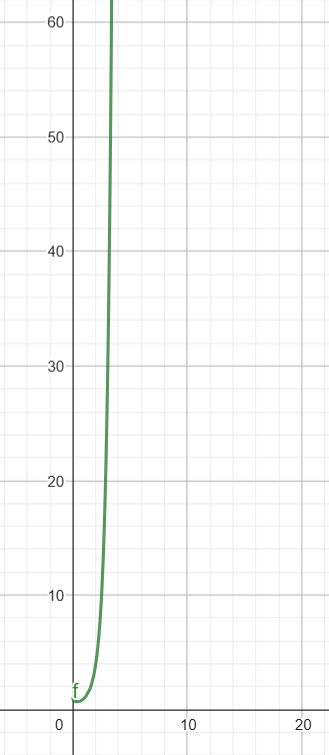
\includegraphics[height=12cm]{GraficoKelevK.png}
\caption{Gráfico da função $k^k$}
\label{fig:kelevk}
\end{figure}

O propósito do algoritmo então é garantir que o tempo possa ser diminuído de acordo com $k$, sem que seja necessário executar para todo $n-k$ restante.

\subsection{Explicação}
O algoritmo é dividido em duas funções principais, a \texttt{main} e a \texttt{defensiveAlliance}. A \texttt{main} recebe como entrada um Grafo $G$ e o tamanho da aliança desejada, um inteiro positivo $k$. De forma intuitiva, a abordagem do algoritmo é partir de um vértice do grafo por vez e olhar sua vizinhança numa tentativa de expandi-lo até formar uma aliança defensiva de tamanho $k$, ou todos os vértices terem servido de raiz da expansão.

\lstset{ 
  deletekeywords={do}  
}

\begin{lstlisting}[escapeinside={(*}{*)}]
Main(G,k)
	Para cada vértice v de G:
		v.c_w <- (*$\ceil{\frac{d(v)}{2}}$*).
	Para cada vértice v de G:
		inicia uma aliança S <- {v}.
		aliança_encontrada <- DefensiveAlliance(S).
		Se aliança_encontrada:
			retorne aliança_encontrada.
		retira v de S
		soma 1 ao c_w de v.
			
	retorne "Sem aliança";
\end{lstlisting}

O papel da função \texttt{main} é garantir que todos os vértices foram usados como raiz da expansão. Para isso, primeiro é definido o \texttt{c\_w}, que serve para verificar se o vértice está protegido dentro da aliança \texttt{S}. De início, ela é definida com o número de vizinhos necessários dentro de $S$ para que ele esteja defendido, e então será aumentada ou diminuida conforme se adiciona ou remove seus vizinhos a $S$.

Isso também faz parte da condição de sucesso da busca, ou seja, quando todos os vértices de \texttt{S} estiverem protegidos (\texttt{c\_w <= 0}) então uma aliança defensiva foi formada.

A seguir, a \texttt{main} chama a função \texttt{defensiveAlliance} para verificar se \texttt{S} é, ou pode ser expandida até, uma aliança defensiva de tamanho \texttt{k}.

\begin{lstlisting}[escapeinside={(*}{*)}]
DefensiveAlliance(G, S, k)
	inicia v <- vértice de maior c_w em S.
	Se v.c_w <= 0 e tamanho de S == k:
		devolve S.
		
	Se v.c_w <= k - tamanho de S: 
		inicia t <- 1 + metade dos vizinhos de w.
		inicia o conjunto W <- t vizinhos de w que não pertencem a S.
		Para cada vértice w em W:
			S <- S + w.
			Para cada vizinho x de w em S:
				subtrai 1 do c_w de x e de w.
			aliança_encontrada <- DefensiveAlliance(G, S, k)
			Se aliança_encontrada:
				Devolve aliança_encontrada.
			Para cada vizinho x de w em S:
				soma 1 ao c_w de x e de w.
			Retira w de S.
			
	Retorne NULL;
\end{lstlisting}

No início de \texttt{defensiveAlliance} o algoritmo escolhe o vértice de maior \texttt{c\_w} em \texttt{S},  que seria o vértice mais vulnerável da aliança. Esse vértice serve para tanto verificar se \texttt{S} se tornou uma aliança quanto como ponto de expansão a fim de incluir novos vértices.

A seguir, o algoritmo verifica se há espaço em \texttt{S} para os \texttt{c\_w} vizinhos necessários serem adicionados, ou seja, para que \texttt{w} seja defendido dentro da restrição do tamanho máximo \texttt{k}. Essa verificação funciona de modo semelhante a uma heurística de busca, poupando tempo ao evitar vértices que não podem ser defendidos posteriormente.

\subsection{Lema 14}
Uma parte importante do funcionamento do algoritmo é o lema 14 de \cite{Enciso2009}. Assuma que $S \subseteq V$ é estendível para uma aliança defensiva S', onde $|S| <|S'| = k$ então, para qualquer vértice desprotegido $w \in S$, $|S' \cap (N[w] - S|) \ge c_w$.\\
Em outras palavras se $S$ é estendível e $w$ é um vértice desprotegido de $S$ então $c_w$ é o número de vizinhos de $w$ fora de $S$ que é necessário para proteger $w$ em $S$.

Esse lema é o que podemos considerar como o núcleo do algoritmo, pois ele nos garante também que para qualquer subconjunto $W \subseteq N[w] - S$ com $t = \lfloor \frac{d_w}{2} \rfloor + 1$  vértices contém ao menos um vértice $w_i$ para o qual $S \cup {w_i}$ é estendível se e somente se S é estendível.

\subsection{Evitando repetir conjuntos}
Observando o comportamento do algoritmo no visualizador web foi possível notar que um comportamento pouco eficiente: o critério de expansão de $S$ (destacado a seguir) abre margem pra repetir várias vezes a mesma combinação de vértices, levando, principalmente em grafos de grande quantidade de vértices, a muito esforço improdutivo.

\begin{lstlisting}
DefensiveAlliance(G, S, k)
	inicia v <- vértice de maior c_w em S.
\end{lstlisting}

Pensando nisso a equipe elaborou uma solução que armazena todas as combinações já analisadas anteriormente e impede de que novas iterações com elas sejam geradas, cortando toda a sub-árvore subsequente. Isso é feito com a criação de um dicionário e a marcação única de cada combinação:

\begin{lstlisting}
inicia combinacoes <- dicionário vazio
\end{lstlisting}

\begin{lstlisting}
DefensiveAlliance(G, S, k)
[...]
	Para cada vértice w em W:
		S <- S + w.
		
		comb_id <- identificadores de S de forma ordenada.
		Se existe combinacoes[comb_id]:
			Retira w de S.
			pula para o próximo vértice.
		Caso contrário:	
			cria combinacoes[comb_id].

		Para cada vizinho x de w em S:
			subtrai 1 do c_w de x e de w.
		aliança_encontrada <- DefensiveAlliance(G, S, k)
[...]
\end{lstlisting}

Caso não exista uma entrada da combinação no dicionário, cria-se uma e a instância corrente de \texttt{S} é analisada. Caso contrário, a instância é ignorada, podando todas as sub-árvores subsequentes. A complexidade de tempo é se resume a ordenação de, no máximo, $k-1$ elementos, e ao acesso e escrita no dicionário. Ambos são ofuscados pela complexidade geral.

Por outro lado, há um custo sério em termos de espaço. No pior caso, de não haver aliança e o algoritmo analisar todos os vértices e $k=n$, a combinação ocupa espaço $O(2^n)$, que corresponde a guardar todas as combinações de $n$ vértices, variando de tamanho $1$ até $n$. Isso pode ser mitigado ao limitar o tamanho das combinações armazenadas para a região crítica que vai ser repetida mais vezes. A análise desta região está na seção sobre Resultados e discussão.

Quanto ao desempenho, esta técnica permite ao algoritmo poupar muito tempo ao "amortizar" o custo $k^k$ ao longo de várias iterações, pois, como nenhuma combinação é repetida, quanto mais exploradas são as combinações dos vértices, menos combinações existem para serem analisadas.

\subsection{Priorização dos vértices expostos}
\begin{lstlisting}
DefensiveAlliance(G, S, k)
	inicia v <- vértice de maior c_w em S.
\end{lstlisting}

Ao iniciarmos $DefensiveAlliance(G,S,k)$ atribuindo $v$ o vértice em $W$ com maior $c_w$ nós garantimos que a maior prioridade em cada chamada recursiva da função é proteger o vértice mais "exposto".

Assim obtemos também um critério de parada consistente, ou seja, quando o vértice com maior $c_w$ ter $c_w \le 0$ e $|S| = k$, teremos duas informações fundamentais sobre o contexto da execução:\\
1 - Se $c_w \le 0$, então todos os vértices em $S$ estão protegidos.\\
2 - Se $|S|=k$, encontramos a aliança defensiva procurada.

\chapter{Metodologia}
O projeto é composto por duas partes principais: algoritmos de busca implementados em Python e um visualizador web criado para exibir os passos deste algoritmo. As partes funcionam de forma independente, sendo conectadas apenas pelo formato de entrada e saída dos programas.

\section{Algoritmo em Python}
A implementação do algoritmo proposto por \cite{Enciso2009} foi feita em Python e consta completa no Apêndice 1.

Nesta implementação foi utilizada a estrutura de dados da biblioteca \textit{Networkx} para manipulação dos grafos, e, no mais, estruturada de forma semelhante ao algoritmo teórico, com a exceção do uso de uma estrutura de pilha para substituir a chamada recursiva.

Além do resultado final, o programa possibilita o retorno da aliança em formato JSON, com as características utilizadas no visualizador web. Essas características permitem a visualização passo a passo dos nós expandidos pelo algoritmo, e consistem do conjunto $W$ a cada iteração da função \texttt{DefensiveAlliance}.

Há também \textit{flags} para mostrar a quantidade de nós expandidos, para gerar um grafo aleatório segundo uma densidade especificada, e para alterar o comportamento da busca, como retornar a primeira aliança encontrada independente do tamanho.

\section{Visualizador web}
O projeto web foi desenvolvido com Typescript e React, e sua proposta é fornecer uma visualização passo-a-passo do algoritmo e do grafo de entrada. Assim como o algoritmo de busca, o visualizador pode ser encontrado no repositório que se encontra nas referências.

Para montar a visualização é necessário que seja fornecido como entrada um grafo disposto em formato JSON, contando com dois conjuntos extras de dados que são a aliança encontrada, caso exista, e um vetor de \textit{steps}, que contém o conjunto $W$ no dado \textit{passo} da iteração.

Munido destas informações, o visualizador organiza os dados internamente para melhorar o desempenho e a decisão de cada caraterística visual do grafo e então personaliza uma \textit{view} HTML, dada pela biblioteca 3d-force-graph \cite{HassanShafique2004}, que cuida da renderização e simulação física do grafo.

Dentre as funcionalidades, vale destacar duas principais: a visualização do conjunto $S$ a cada etapa do algoritmo e o mapa de calor dos nós explorados. O mapa de calor é a coloração dos vértices do grafo seguindo a regra de que, quanto mais visitado um vértice durante a execução do algoritmo, mais quente é a cor usada; os nós mais quentes tem cores próximas do vermelho, e os mais frios, mais próximas do azul.

\subsection{Visualização por passos}
Ao carregar um grafo com o conjunto de passos, é possível navegar por cada um deles. Em um certo passo, os vértices e arestas da fronteira de $S$ são desenhados com uma cor cinza escura, os além da fronteira tem cor cinza claro, e os vértices dentro de $S$ ficam coloridos com a cor

\begin{itemize}
  \item azul, se estiverem desprotegidos;
  \item ou verde, se estiverem devidamente protegidos.
\end{itemize}

Ao finalizar o algoritmo e desenhar a aliança, ela é colorida de verde escuro.

As figuras a seguir são de uma busca por uma aliança de tamanho $k = 15$ em um grafo de $v=50$ vértices e $e=40$ arestas. O algoritmo começa com $S$ contendo o vértice colorido de azul.

\begin{figure}[!htb]
\centering
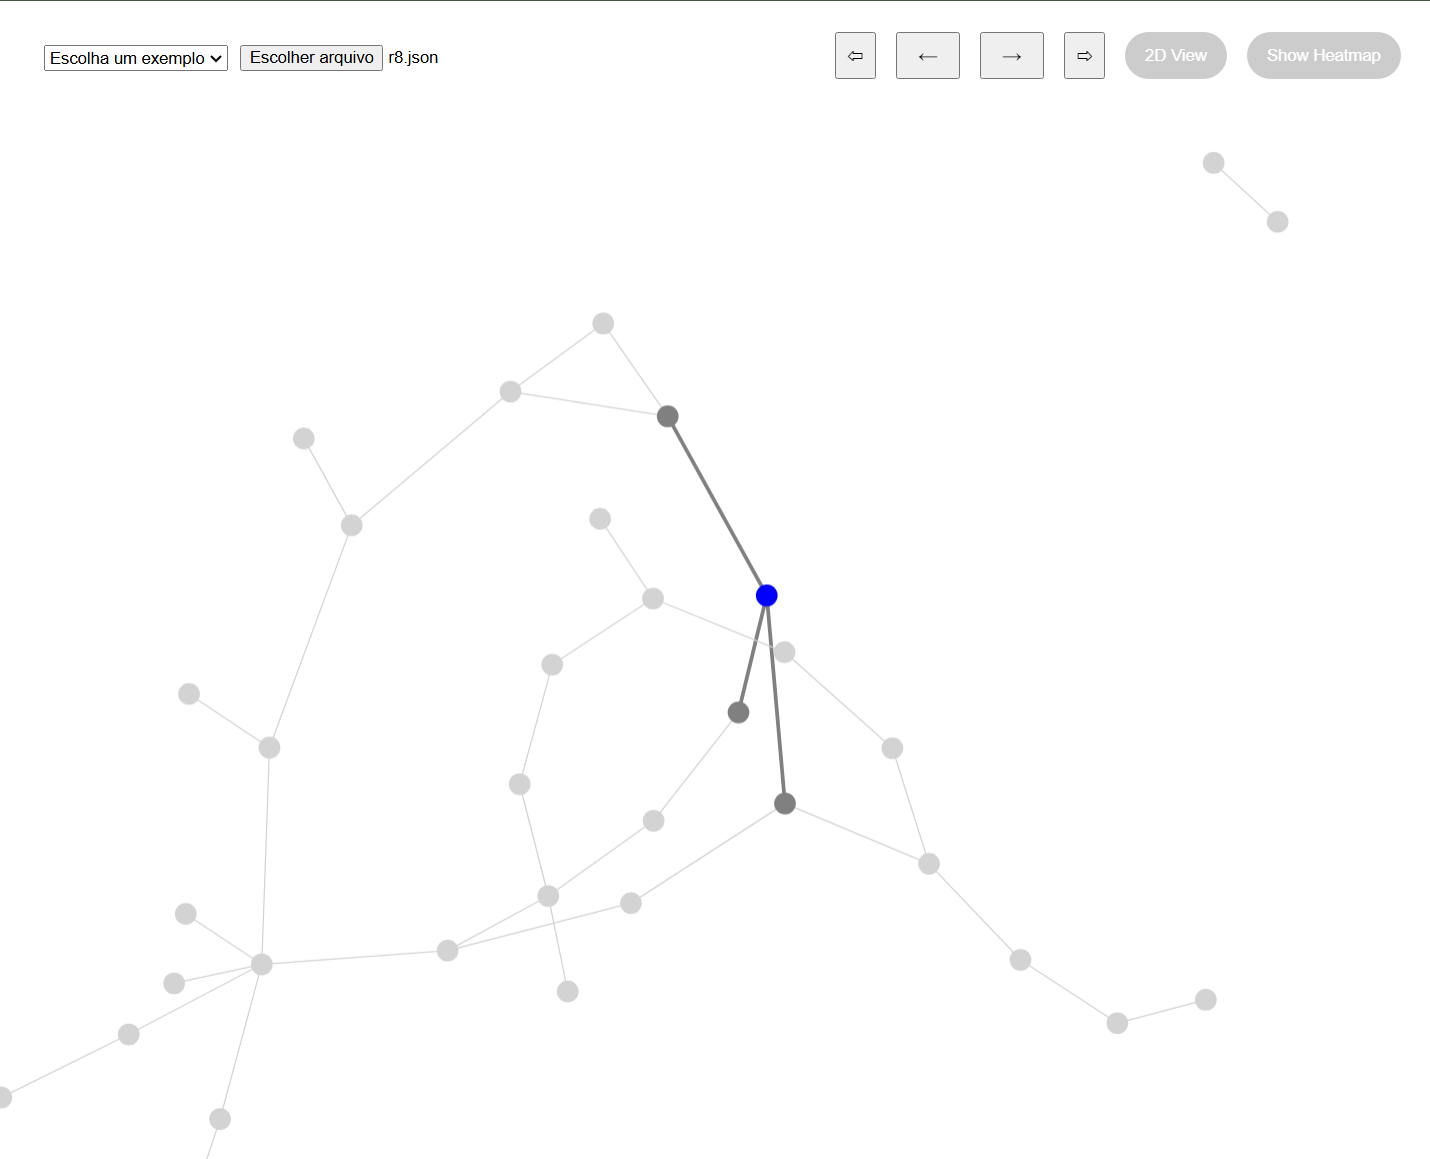
\includegraphics[width=12cm]{GrafoSteps1.png}
\caption{Passo 1 do algoritmo}
\label{fig:grafo-steps-1}
\end{figure}

\begin{figure}[!htb]
\centering
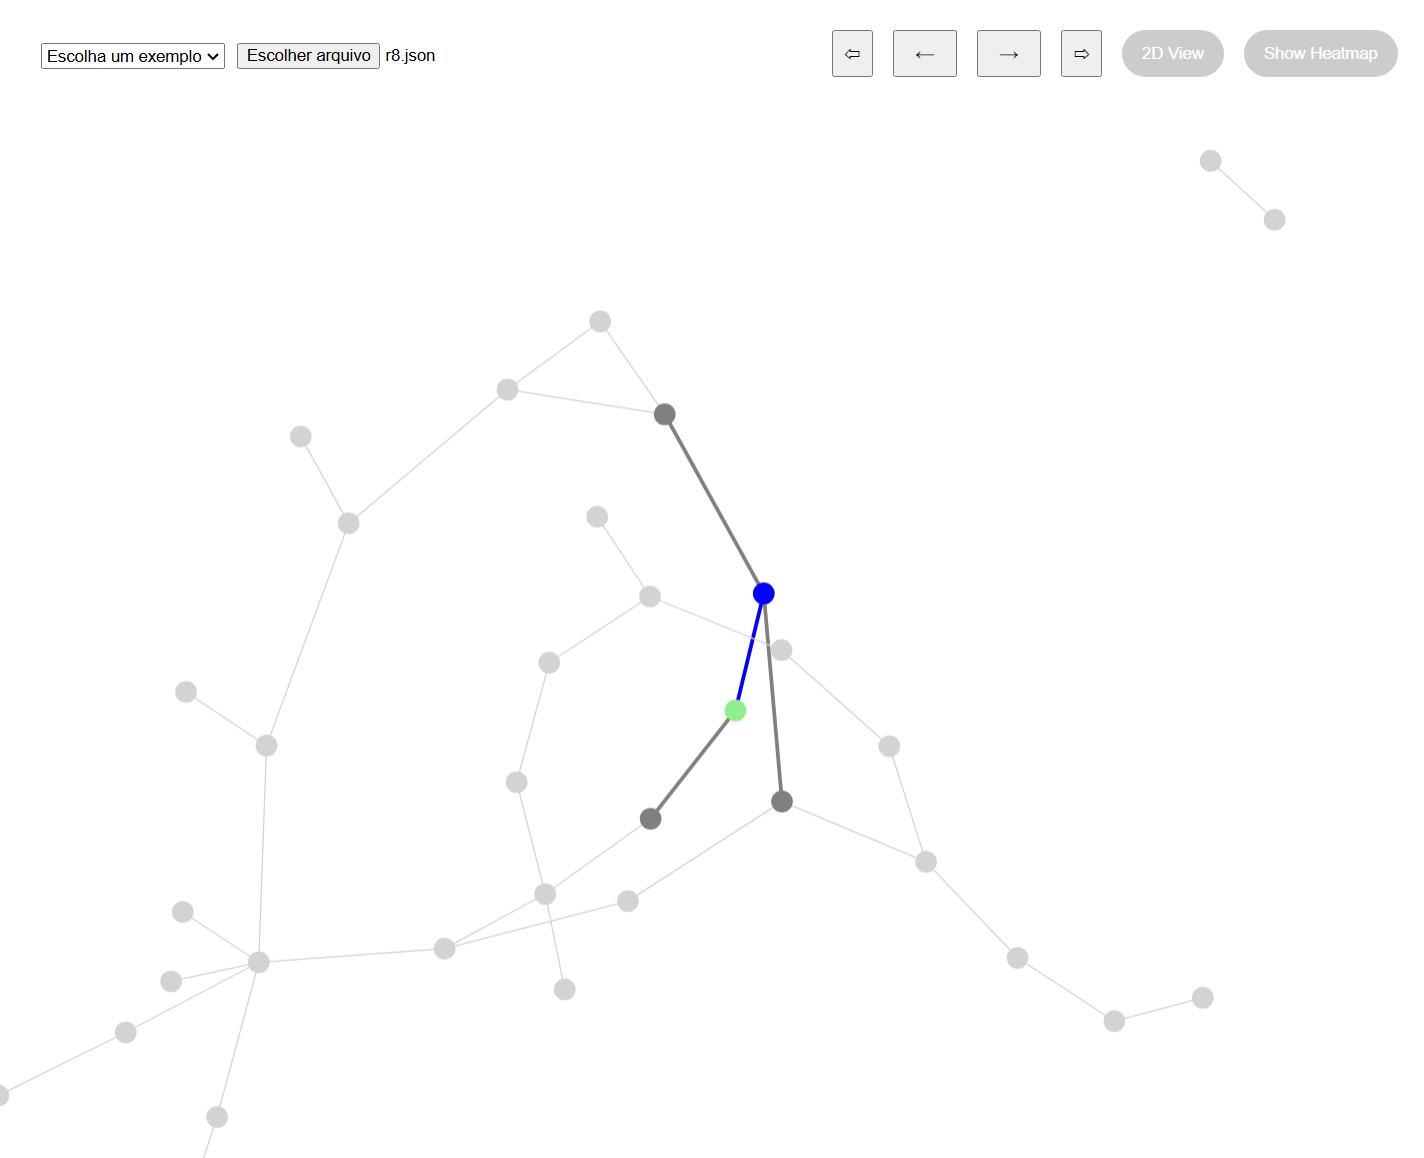
\includegraphics[width=12cm]{GrafoSteps2.png}
\caption{Passo 2 do algoritmo}
\label{fig:grafo-steps-2}
\end{figure}

\begin{figure}[!htb]
\centering
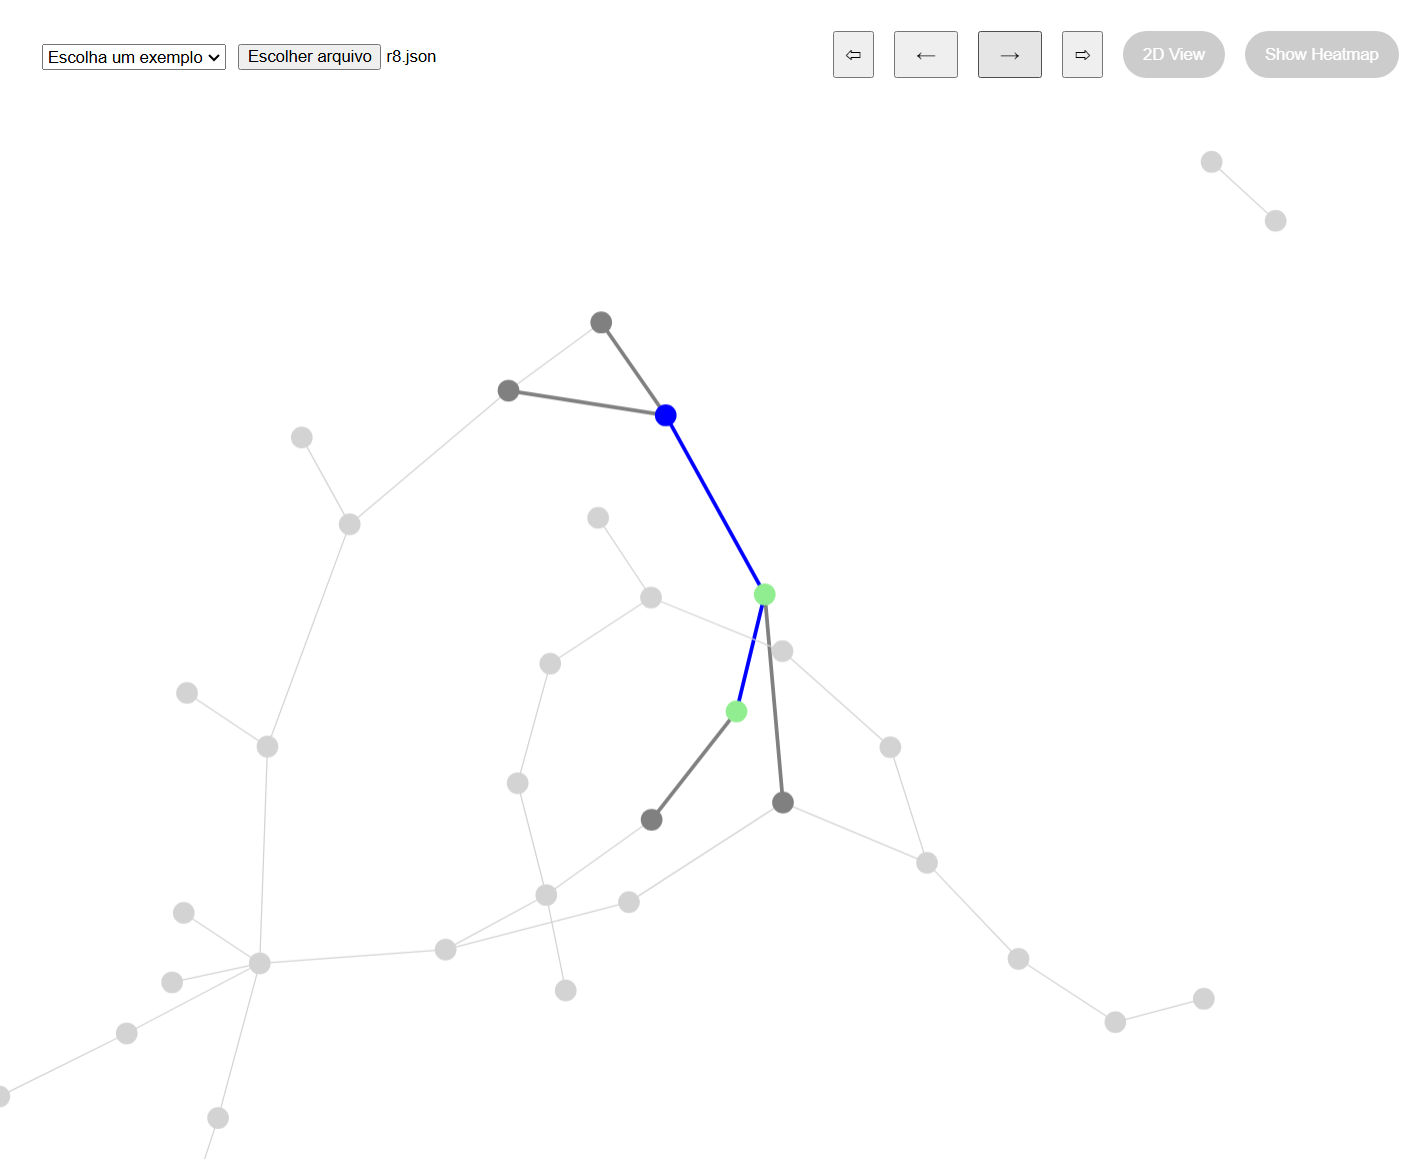
\includegraphics[width=12cm]{GrafoSteps3.png}
\caption{Passo 3 do algoritmo}
\label{fig:grafo-steps-3}
\end{figure}

\begin{figure}[!htb]
\centering
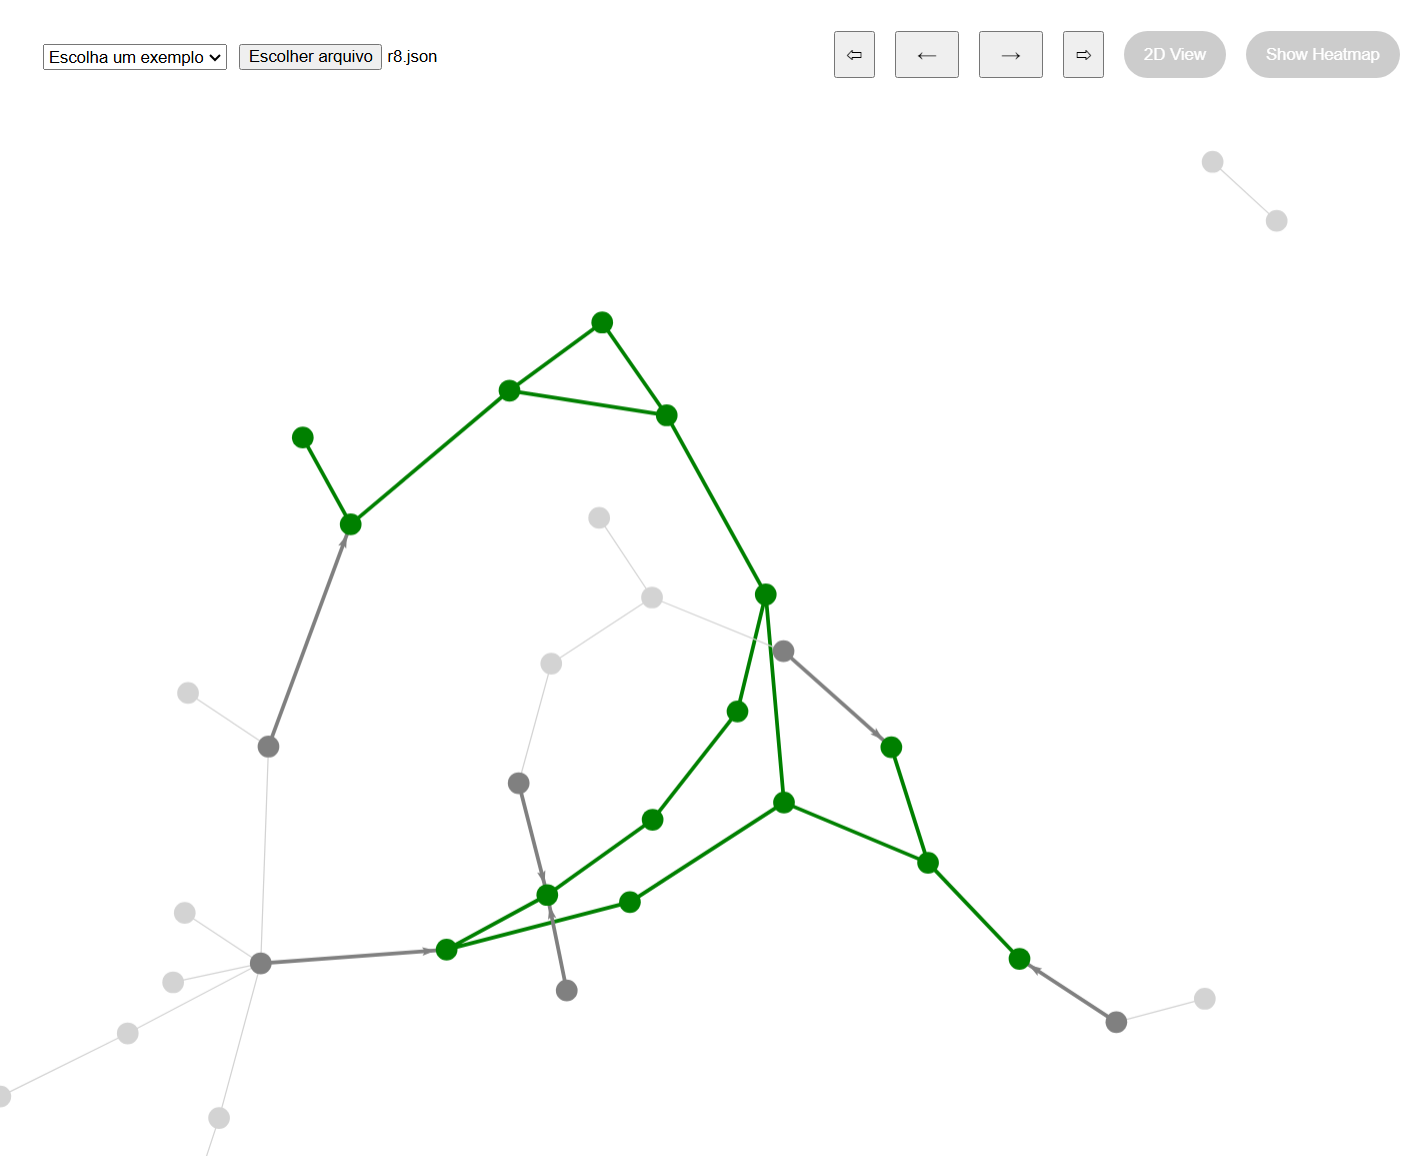
\includegraphics[width=12cm]{GrafoStepsN.png}
\caption{Passo final do algoritmo}
\label{fig:grafo-steps-n}
\end{figure}

\subsection{Mapa de calor}
É possível também ativar a visualização do mapa de calor, que colore os vértices de acordo com a quantidade de vezes que ele foi explorado pelo algoritmo.

\begin{figure}[!htb]
\centering
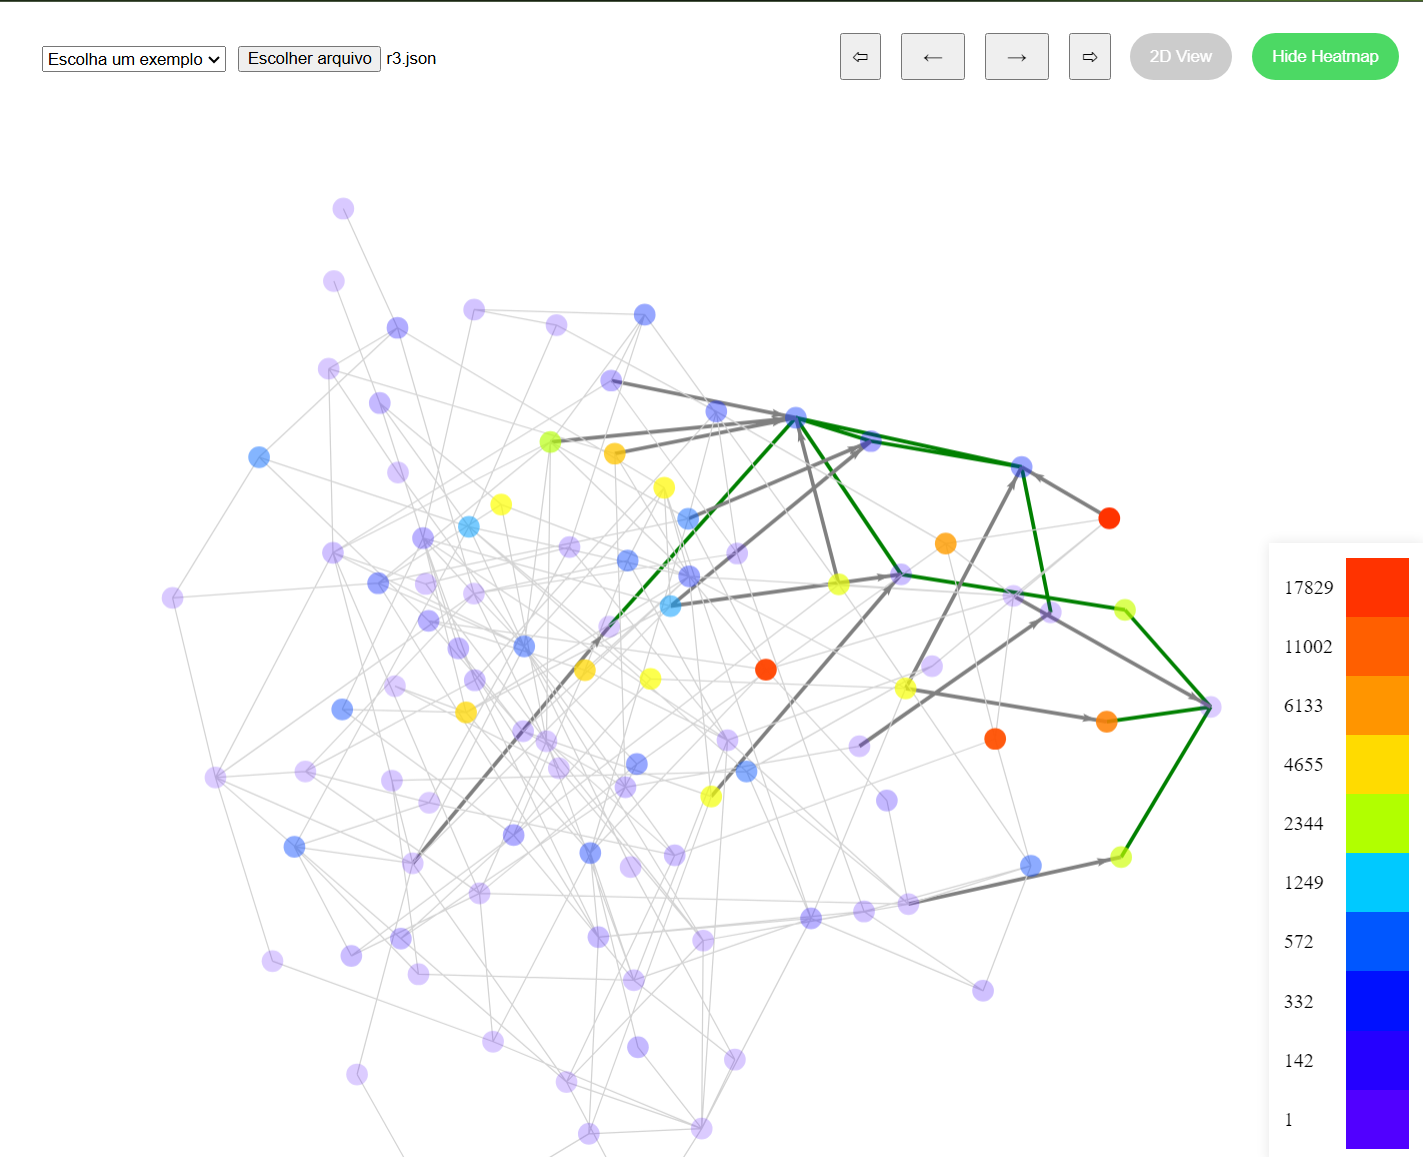
\includegraphics[width=12cm]{GrafoHeatmap.png}
\caption{Mapa de calor do grafo}
\label{fig:grafo-heatmap}
\end{figure}

Para ajudar na visualização, as cores mais frias também tem opacidade mais baixa.

Essa ferramenta em particular incentivou questionamentos interessantes a respeito da eficiência do algoritmo, como "como evitar a alta taxa de repetição de um grupo de vértices".

\chapter{Resultados e discussão}
O algoritmo originalmente estudado e a versão com as melhorias propostas foram analisadas e submetidas a um conjunto de testes para melhor ilustrar o impacto e eficiência de cada uma. Visto que o problema continua sendo NP-completo, há pouco a ser feito para valores realmente grandes, mas foi possível sim observar uma ampliação dos valores considerados "razoáveis" pelo algoritmo FPT.

Para testar o algoritmo utilizamos a função da biblioteca \texttt{networkx nx.erdos\_renyi\_graph(v,e,seed)} onde \texttt{v} é o número de vértices \texttt{e} é a probabilidade de 2 vértices formarem uma aresta, e \texttt{seed} é uma semente para geração do Grafo.

Para os testes a seguir foram fixados os seguintes seguintes parâmetros \texttt{v=30} \texttt{e=0.333} e \texttt{seed=100} e executamos para \texttt{k} variando entre \texttt{1} e \texttt{29}.

\begin{figure}[!htb]
\centering
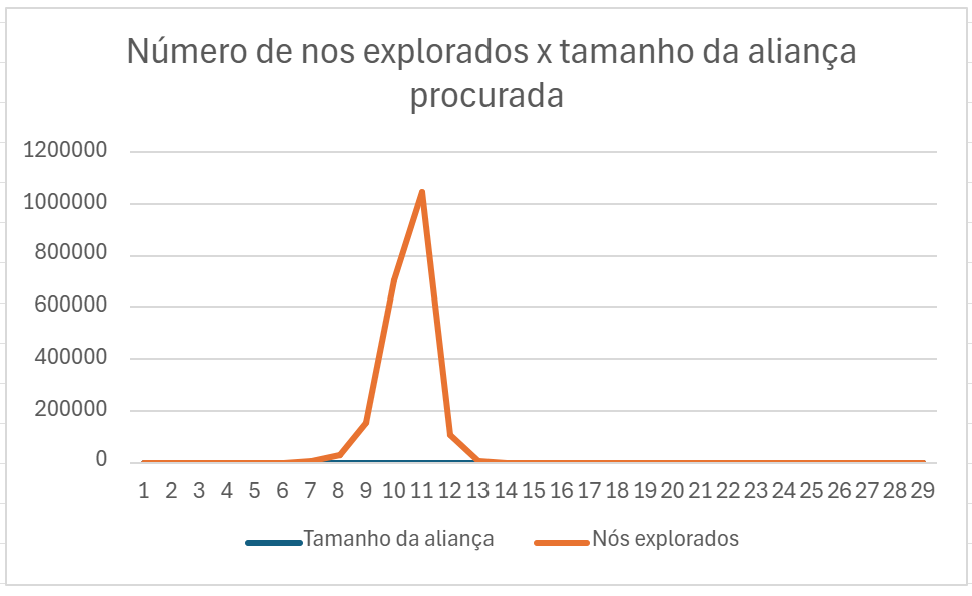
\includegraphics[width=12cm]{Execução sem repetição de conjuntos.png}
\caption{Execução do algoritmo \textbf{evitando} a repetição de conjuntos}
\label{fig:execucao-sem-repeticao}
\end{figure}

Na execução do algoritmo sem repetição de conjuntos é possível notar que o número máximo de nós explorados foi de aproximadamente 1 milhão de nós.

\begin{figure}[!htb]
\centering
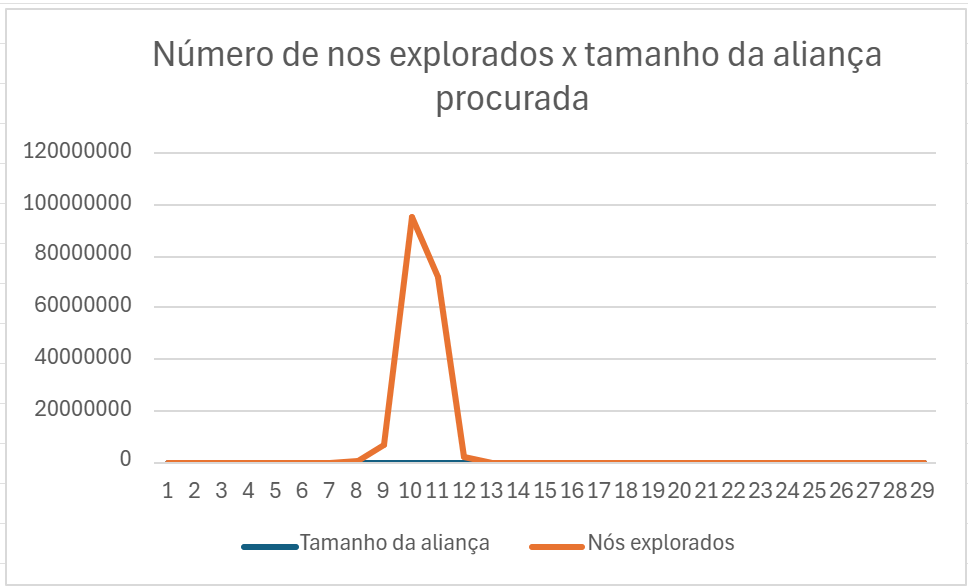
\includegraphics[width=12cm]{Execução com repetição de conjuntos.png}
\caption{Execução do algoritmo \textbf{permitindo} a repetição de conjuntos}
\label{fig:execucao-com-repeticao}
\end{figure}

Por sua vez, na execução que permite a repetição de conjuntos o número de nós explorados nesse caso saltou de 1 milhão para 100 milhões.

Salvar os conjuntos resulta em uma melhora significativa na redução do número de nós a serem explorados, porém nós traz um novo problema pois o espaço necessário para armazenar todos esses conjuntos no pior caso é $\sum_{i=0}^{k} \binom{n}{i}<2^n$, ou seja, acabamos trocando um tempo exponencial, por espaço exponencial.

Foi observado um padrão interessante na eficiência com relação ao grau médio dos vértices do grafo $d(G)$ e $k$; o número de nós explorados atinge um ápice para valores de $k$ próximos de $d(G)$ criando uma "zona difícil", e suaviza a medida que a diferença aumenta.

Para valores de $d(G)$ muito maiores que $k$ isso acontece porque o algoritmo pode descartar muitas combinações através do critério \texttt{Se v.c\_w <= k - tamanho de S:}. Essa linha garante que o próximo nó a ser expandido ao menos tem as condições de ser protegido dado o tamanho atual de $S$.

Por outro lado, valores de $k$ muito menores do que $d(G)$, foi observado uma probabilidade maior de haver uma aliança defensiva. A modificação de ordenação dos vértices de \texttt{W} com base em quantos vizinhos ele possui em $S$ e $\lfloor d(v)/2 \rfloor$, em especial, mostrou acelerar muito o processo de determinação da aliança, quando existente. Isso se deve as escolhas priorizarem a defesa dos vértices já em $S$, em prol de adições aleatórias.

Por fim, a modificação de "Evitar repetir conjuntos" mostrou-se acelerar o processo tanto no melhor caso quanto no pior, pois garante que somente novas combinações são testadas.

\chapter{Conclusão}
O estudo como um todo foi bastante produtivo dentro do tema, e possibilitou compreensão significativa do que são e como encontrar alianças defensivas. O visualizador web, como ferramenta didática, foi bastante aproveitado para a compreensão e elaboração das melhorias propostas ao algoritmo.

Também foi produtivo experimentar na prática a complexidade de um problema NP-completo e uma das ferramentas usadas para contornar esse degrau gigantesco na complexidade.

Dentre os diversos temas que podem ser abordados em discussões futuras, destacamos a implementação e análise do algoritmo proposto por \cite{Enciso2009} para encontrar Conjuntos Seguros (\textit{Secure Sets}), que segue uma abordagem FPT semelhante ao de alianças defensivas, e pode ser adaptado para o visualizador web para gerar resultados valiosos.

Outro ponto de possível expansão é o de pré-análise de grafos para a determinação de potencial de uma aliança de tamanho $k$, partindo da análise feita sobre o grau médio e a "zona difícil".
		% fundamentação teórica
%\chapter{Fundamentação teórica}
A fim de seguir de forma devida com a análise do problema e do algoritmo, algumas definições teóricas são requeridas:

\section{Conceitos}

\subsection{Grafo}
Um grafo $G = (V(G), E(G))$ é um par ordenado que consiste de um conjunto de vértices $V(G)$ e um conjunto de arestas $E(G)$.

\subsection{Vértice}
Um vértice $v \in V(G)$ é um elemento básico de um grafo, representando um ponto ou nó na estrutura. O conjunto $V(G)$ é finito e contém todos os vértices do grafo.

\subsection{Aresta}
Uma aresta $e \in E(G)$ é um conjunto de dois vértices de $V(G)$. Em um grafo não direcionado, a aresta $\{u, v\}$ conecta os vértices $u$ e $v$, sem direção. Em grafos direcionados, uma aresta $(u, v)$ conecta $u$ a $v$ com uma orientação de $u$ para $v$.

\subsection{Incidência}
As extremidades de uma aresta são ditas incidentes com a aresta \cite{Bondy2008}, e vice-versa, ou seja, uma aresta $e$ é dita incidente a um vértice $v$ se está aresta se conecta a $v$ em um de seus extremos.

\subsection{Adjacência}
Dois vértices que são incidentes a uma mesma aresta são adjacentes \cite{Bondy2008}, assim como duas arestas que são incidentes a um mesmo vértice, ou seja, um par de vértices distintos $u$ e $v$ são adjacentes se possuem uma aresta que os conectam, da mesma forma que duas arestas distintas $e1$ e $e2$ são adjacentes se são incidentes a um vértice em comum.

\subsection{Vizinhança de um Vértice}
Dois vértices que são incidentes a uma aresta comum, ou seja, dois vértices adjacentes distintos são ditos vizinhos \cite{Bondy2008}. A vizinhança de um vértice $v \in V(G)$, denotada por $N(v)$, é o conjunto de todos os vértices adjacentes a $v$, ou seja, $N(v) = \{ u \in V(G) \mid \{u, v\} \in E(G) \}$ em grafos não direcionados.

\subsection{Grau de um Vértice}
O grau de um vértice $v$ em um grafo não direcionado $G$ é dado por $d(v) = |N(v)|$, ou seja, o número de arestas incidentes a $v$. Neste estudo consideramos apenas grafos não direcionados, portanto o grau de $v$ corresponde ao número de arestas total ligadas a ele.

\subsection{Subgrafo}
Um \textbf{subgrafo} de um grafo $G$ é um grafo $F$ cujos conjuntos de vértices e arestas são subconjuntos dos vértices e arestas de $G$. Formalmente, $F$ é um subgrafo de $G$ se $V(F) \subseteq V(G)$ e $E(F) \subseteq E(G)$, e a função que relaciona vértices e arestas em $F$ é a mesma que em $G$, mas restrita ao conjunto de arestas de $F$. Subgrafos podem ser formados a partir das operações de remoção de vértices e remoção de arestas.\\
Diz-se que $G$ contém $F$ ou que $F$ está contido em $G$, representado como $G \supseteq F$ ou $F \subseteq G$.

\subsection{Conectividade}
Um grafo é \textbf{conexo} se, para toda partição de seu conjunto de vértices em dois conjuntos não vazios $X$ e $Y$, existe uma aresta com uma extremidade em $X$ e a outra extremidade em $Y$, caso contrário, o grafo é desconexo. Em outras palavras, um grafo é desconexo se seu conjunto de vértices pode ser particionado em dois subconjuntos não vazios $X$ e $Y$ de modo que nenhuma aresta tenha uma extremidade em $X$ e outra em $Y$.

\subsection{Aliança Defensiva}
Um subconjunto $S \subseteq V$ é uma aliança defensiva se, para cada vértice $v \in S$, a condição a seguir é satisfeita:   $|N(v) \cap S| \geq |N(v) \setminus S|$.\\
Ou seja, para cada vértice $v$ na aliança $S$, o número de vértices adjacentes a $v$ dentro de $S$ deve ser pelo menos igual ao número de vértices adjacentes a $v$ fora de $S$.\\
Isso indica que os vértices $v$ na aliança devem possuir pelo menos tantos vértices dentro da aliança quanto fora dela.\\
Embora, formalmente, uma aliança não precise ser conexa, note que cada componente conexa de uma aliança é uma aliança por si só. Para fins deste trabalho, toda aliança encontrada deve ser \textbf{conexa}.

\section{Complexidade Computacional}
A complexidade computacional estuda a quantidade de recursos necessários para a execução de algoritmos, especialmente em termos de tempo e espaço. Em ciência da computação, a complexidade computacional é frequentemente representada usando a notação \textit{Big O}, $O(f(n))$, que descreve o crescimento da complexidade como uma função $f(n)$, onde $n$ normalmente é o tamanho da entrada, ou algum outro parâmetro relevante. Alguns exemplos de classificação de complexidade são:

\begin{itemize}
  \item $O(1)$: Constante, o tempo de execução não depende do tamanho da entrada.
  \item $O(n)$: Linear, o tempo de execução cresce proporcionalmente ao tamanho da entrada.
  \item $O(n^k)$: Polinomial, o tempo de execução cresce proporcionalmente com relação a potência $k$ constante do tamanho da entrada. Um exemplo de polinômio muito comum são os quadrados $O(n^2)$.
  \item $O(k^n)$: Exponencial, o tempo de execução cresce de forma exponencial com relação ao tamanho da entrada. No geral, é inviável para grandes entradas.
  \item $O(n!)$ Fatorial, em problemas fatoriais o tempo de execução cresce ainda mais acelerado com relação ao tamanho da entrada do que problemas exponenciais.
\end{itemize}

\subsection{Classes de Complexidade:}
Os problemas de decisão, como os envolvendo alianças, podem ser classificados em certas classes de complexidade que separam o quão viáveis é encontrar ou verificar suas soluções para entradas de larga escala. Estas classes não:

\begin{itemize}
  \item $P$ (Polinomial): Representa a classe de problemas que podem ser resolvidos em tempo polinomial, ou seja, em $O(n^k)$ para algum inteiro $k$. Em ciência da computação, problemas em $P$ são considerados tratáveis.
  \item $NP$ (Tempo polinomial não determinístico): Representa a classe de problemas para os quais, apesar de não sabermos como encontrar solução em tempo polinomial de maneira determinística, dada uma solução, ela pode ser verificada em tempo polinomial por um algoritmo determinístico. Não sabemos se todo problema em $NP$ pode ser resolvido em tempo polinomial, isto é, se $P = NP$, e esse é um dos 7 problemas do milênio que ainda estão em aberto.
  \item $NP$-completo: Representa um subconjunto de problemas em $NP$ que são, intuitivamente, tão difíceis quanto qualquer outro problema em $NP$. Para um problema ser dessa classe, são necessárias duas características:
  \begin{enumerate}
    \item Estar em $NP$, ou seja, dada uma solução, ela deve ser verificável em tempo polinomial.
    \item Ser $NP$-difícil, todo problema em $NP$ pode ser redutível a ele em tempo polinomial.\\
Em outras palavras, caso um problema de classe $NP$-completo seja resolvido em tempo polinomial, todos os outros problemas em $NP$ poderão ser resolvidos em tempo polinomial.
  \end{enumerate}
\end{itemize}

\section{O algoritmo}
Como encontrar uma aliança defensiva em um grafo é um problema NP-completo, o algoritmo FPT \cite{Enciso2009} tem como objetivo buscar por uma aliança conexa arbitrária de tamanho máximo $k$, a fim de tornar o problema tratável. Porém, neste trabalho o tamanho da aliança buscada será \textit{exatamente} $k$, pois acreditamos que o tamanho da aliança seja importante. Antes de entrar na explicação minuciosa do algoritmo, é importante explicar o que é um algoritmo FPT.

\subsection{Complexidade}
FPT (\textit{Fixed-Parameter Tractable}) é uma classe de complexidade que trata de problemas parametrizáveis (como os de complexidade exponencial) ao isolar e fixar um parâmetro específico do problema, chamado $k$, e então expressando a complexidade na forma $f(k)*p(n).$ Desta forma, $f(k)$ é a parte da complexidade que depende exclusivamente de $k$ e pode ser \textit{superpolinomial}, enquanto $p(n)$ é uma função polinomial de $n$. Sendo assim, fixar $k$ em valores pequenos nos permite abordar o algoritmo de forma mais tratável, custando muito menos tempo, a depender do tamanho de $k$.

O algoritmo usado neste estudo foi proposto por \cite{Enciso2009}, e tem complexidade $O(k^kn)$, e é uma melhora significativa de seu predecessor, que tinha complexidade $O((2k-1)^kk^2n)$. Esse é um avanço substancial, mas ainda é interessante demonstrar como problemas, mesmo parametrizados, crescem rapidamente:

\begin{table}[h]
\begin{center}
\begin{tabular}{|c|c|c|c|c|c|c|c|}
\hline
$k$ & $k^k$\\
\hline
2 & 4 \\
\hline
3 & 27 \\
\hline
4 & 256 \\
\hline
5 & 3.125 \\
\hline
6 & 46.656 \\
\hline
7 & 823.543 \\
\hline
9 & 387.420.489 \\
\hline
10 & 10.000.000.000 \\
\hline
\end{tabular}
\end{center}
\end{table}

\begin{figure}[!htb]
\centering
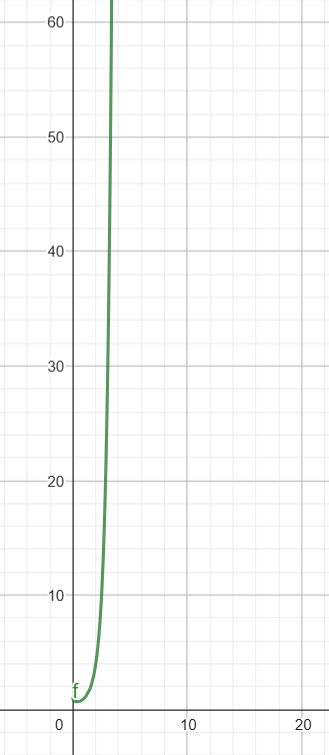
\includegraphics[height=12cm]{GraficoKelevK.png}
\caption{Gráfico da função $k^k$}
\label{fig:kelevk}
\end{figure}

O propósito do algoritmo então é garantir que o tempo possa ser diminuído de acordo com $k$, sem que seja necessário executar para todo $n-k$ restante.

\subsection{Explicação}
O algoritmo é dividido em duas funções principais, a \texttt{main} e a \texttt{defensiveAlliance}. A \texttt{main} recebe como entrada um Grafo $G$ e o tamanho da aliança desejada, um inteiro positivo $k$. De forma intuitiva, a abordagem do algoritmo é partir de um vértice do grafo por vez e olhar sua vizinhança numa tentativa de expandi-lo até formar uma aliança defensiva de tamanho $k$, ou todos os vértices terem servido de raiz da expansão.

\lstset{ 
  deletekeywords={do}  
}

\begin{lstlisting}[escapeinside={(*}{*)}]
Main(G,k)
	Para cada vértice v de G:
		v.c_w <- (*$\ceil{\frac{d(v)}{2}}$*).
	Para cada vértice v de G:
		inicia uma aliança S <- {v}.
		aliança_encontrada <- DefensiveAlliance(S).
		Se aliança_encontrada:
			retorne aliança_encontrada.
		retira v de S
		soma 1 ao c_w de v.
			
	retorne "Sem aliança";
\end{lstlisting}

O papel da função \texttt{main} é garantir que todos os vértices foram usados como raiz da expansão. Para isso, primeiro é definido o \texttt{c\_w}, que serve para verificar se o vértice está protegido dentro da aliança \texttt{S}. De início, ela é definida com o número de vizinhos necessários dentro de $S$ para que ele esteja defendido, e então será aumentada ou diminuida conforme se adiciona ou remove seus vizinhos a $S$.

Isso também faz parte da condição de sucesso da busca, ou seja, quando todos os vértices de \texttt{S} estiverem protegidos (\texttt{c\_w <= 0}) então uma aliança defensiva foi formada.

A seguir, a \texttt{main} chama a função \texttt{defensiveAlliance} para verificar se \texttt{S} é, ou pode ser expandida até, uma aliança defensiva de tamanho \texttt{k}.

\begin{lstlisting}[escapeinside={(*}{*)}]
DefensiveAlliance(G, S, k)
	inicia v <- vértice de maior c_w em S.
	Se v.c_w <= 0 e tamanho de S == k:
		devolve S.
		
	Se v.c_w <= k - tamanho de S: 
		inicia t <- 1 + metade dos vizinhos de w.
		inicia o conjunto W <- t vizinhos de w que não pertencem a S.
		Para cada vértice w em W:
			S <- S + w.
			Para cada vizinho x de w em S:
				subtrai 1 do c_w de x e de w.
			aliança_encontrada <- DefensiveAlliance(G, S, k)
			Se aliança_encontrada:
				Devolve aliança_encontrada.
			Para cada vizinho x de w em S:
				soma 1 ao c_w de x e de w.
			Retira w de S.
			
	Retorne NULL;
\end{lstlisting}

No início de \texttt{defensiveAlliance} o algoritmo escolhe o vértice de maior \texttt{c\_w} em \texttt{S},  que seria o vértice mais vulnerável da aliança. Esse vértice serve para tanto verificar se \texttt{S} se tornou uma aliança quanto como ponto de expansão a fim de incluir novos vértices.

A seguir, o algoritmo verifica se há espaço em \texttt{S} para os \texttt{c\_w} vizinhos necessários serem adicionados, ou seja, para que \texttt{w} seja defendido dentro da restrição do tamanho máximo \texttt{k}. Essa verificação funciona de modo semelhante a uma heurística de busca, poupando tempo ao evitar vértices que não podem ser defendidos posteriormente.

\subsection{Lema 14}
Uma parte importante do funcionamento do algoritmo é o lema 14 de \cite{Enciso2009}. Assuma que $S \subseteq V$ é estendível para uma aliança defensiva S', onde $|S| <|S'| = k$ então, para qualquer vértice desprotegido $w \in S$, $|S' \cap (N[w] - S|) \ge c_w$.\\
Em outras palavras se $S$ é estendível e $w$ é um vértice desprotegido de $S$ então $c_w$ é o número de vizinhos de $w$ fora de $S$ que é necessário para proteger $w$ em $S$.

Esse lema é o que podemos considerar como o núcleo do algoritmo, pois ele nos garante também que para qualquer subconjunto $W \subseteq N[w] - S$ com $t = \lfloor \frac{d_w}{2} \rfloor + 1$  vértices contém ao menos um vértice $w_i$ para o qual $S \cup {w_i}$ é estendível se e somente se S é estendível.

\subsection{Evitando repetir conjuntos}
Observando o comportamento do algoritmo no visualizador web foi possível notar que um comportamento pouco eficiente: o critério de expansão de $S$ (destacado a seguir) abre margem pra repetir várias vezes a mesma combinação de vértices, levando, principalmente em grafos de grande quantidade de vértices, a muito esforço improdutivo.

\begin{lstlisting}
DefensiveAlliance(G, S, k)
	inicia v <- vértice de maior c_w em S.
\end{lstlisting}

Pensando nisso a equipe elaborou uma solução que armazena todas as combinações já analisadas anteriormente e impede de que novas iterações com elas sejam geradas, cortando toda a sub-árvore subsequente. Isso é feito com a criação de um dicionário e a marcação única de cada combinação:

\begin{lstlisting}
inicia combinacoes <- dicionário vazio
\end{lstlisting}

\begin{lstlisting}
DefensiveAlliance(G, S, k)
[...]
	Para cada vértice w em W:
		S <- S + w.
		
		comb_id <- identificadores de S de forma ordenada.
		Se existe combinacoes[comb_id]:
			Retira w de S.
			pula para o próximo vértice.
		Caso contrário:	
			cria combinacoes[comb_id].

		Para cada vizinho x de w em S:
			subtrai 1 do c_w de x e de w.
		aliança_encontrada <- DefensiveAlliance(G, S, k)
[...]
\end{lstlisting}

Caso não exista uma entrada da combinação no dicionário, cria-se uma e a instância corrente de \texttt{S} é analisada. Caso contrário, a instância é ignorada, podando todas as sub-árvores subsequentes. A complexidade de tempo é se resume a ordenação de, no máximo, $k-1$ elementos, e ao acesso e escrita no dicionário. Ambos são ofuscados pela complexidade geral.

Por outro lado, há um custo sério em termos de espaço. No pior caso, de não haver aliança e o algoritmo analisar todos os vértices e $k=n$, a combinação ocupa espaço $O(2^n)$, que corresponde a guardar todas as combinações de $n$ vértices, variando de tamanho $1$ até $n$. Isso pode ser mitigado ao limitar o tamanho das combinações armazenadas para a região crítica que vai ser repetida mais vezes. A análise desta região está na seção sobre Resultados e discussão.

Quanto ao desempenho, esta técnica permite ao algoritmo poupar muito tempo ao "amortizar" o custo $k^k$ ao longo de várias iterações, pois, como nenhuma combinação é repetida, quanto mais exploradas são as combinações dos vértices, menos combinações existem para serem analisadas.

\subsection{Priorização dos vértices expostos}
\begin{lstlisting}
DefensiveAlliance(G, S, k)
	inicia v <- vértice de maior c_w em S.
\end{lstlisting}

Ao iniciarmos $DefensiveAlliance(G,S,k)$ atribuindo $v$ o vértice em $W$ com maior $c_w$ nós garantimos que a maior prioridade em cada chamada recursiva da função é proteger o vértice mais "exposto".

Assim obtemos também um critério de parada consistente, ou seja, quando o vértice com maior $c_w$ ter $c_w \le 0$ e $|S| = k$, teremos duas informações fundamentais sobre o contexto da execução:\\
1 - Se $c_w \le 0$, então todos os vértices em $S$ estão protegidos.\\
2 - Se $|S|=k$, encontramos a aliança defensiva procurada.

\chapter{Metodologia}
O projeto é composto por duas partes principais: algoritmos de busca implementados em Python e um visualizador web criado para exibir os passos deste algoritmo. As partes funcionam de forma independente, sendo conectadas apenas pelo formato de entrada e saída dos programas.

\section{Algoritmo em Python}
A implementação do algoritmo proposto por \cite{Enciso2009} foi feita em Python e consta completa no Apêndice 1.

Nesta implementação foi utilizada a estrutura de dados da biblioteca \textit{Networkx} para manipulação dos grafos, e, no mais, estruturada de forma semelhante ao algoritmo teórico, com a exceção do uso de uma estrutura de pilha para substituir a chamada recursiva.

Além do resultado final, o programa possibilita o retorno da aliança em formato JSON, com as características utilizadas no visualizador web. Essas características permitem a visualização passo a passo dos nós expandidos pelo algoritmo, e consistem do conjunto $W$ a cada iteração da função \texttt{DefensiveAlliance}.

Há também \textit{flags} para mostrar a quantidade de nós expandidos, para gerar um grafo aleatório segundo uma densidade especificada, e para alterar o comportamento da busca, como retornar a primeira aliança encontrada independente do tamanho.

\section{Visualizador web}
O projeto web foi desenvolvido com Typescript e React, e sua proposta é fornecer uma visualização passo-a-passo do algoritmo e do grafo de entrada. Assim como o algoritmo de busca, o visualizador pode ser encontrado no repositório que se encontra nas referências.

Para montar a visualização é necessário que seja fornecido como entrada um grafo disposto em formato JSON, contando com dois conjuntos extras de dados que são a aliança encontrada, caso exista, e um vetor de \textit{steps}, que contém o conjunto $W$ no dado \textit{passo} da iteração.

Munido destas informações, o visualizador organiza os dados internamente para melhorar o desempenho e a decisão de cada caraterística visual do grafo e então personaliza uma \textit{view} HTML, dada pela biblioteca 3d-force-graph \cite{HassanShafique2004}, que cuida da renderização e simulação física do grafo.

Dentre as funcionalidades, vale destacar duas principais: a visualização do conjunto $S$ a cada etapa do algoritmo e o mapa de calor dos nós explorados. O mapa de calor é a coloração dos vértices do grafo seguindo a regra de que, quanto mais visitado um vértice durante a execução do algoritmo, mais quente é a cor usada; os nós mais quentes tem cores próximas do vermelho, e os mais frios, mais próximas do azul.

\subsection{Visualização por passos}
Ao carregar um grafo com o conjunto de passos, é possível navegar por cada um deles. Em um certo passo, os vértices e arestas da fronteira de $S$ são desenhados com uma cor cinza escura, os além da fronteira tem cor cinza claro, e os vértices dentro de $S$ ficam coloridos com a cor

\begin{itemize}
  \item azul, se estiverem desprotegidos;
  \item ou verde, se estiverem devidamente protegidos.
\end{itemize}

Ao finalizar o algoritmo e desenhar a aliança, ela é colorida de verde escuro.

As figuras a seguir são de uma busca por uma aliança de tamanho $k = 15$ em um grafo de $v=50$ vértices e $e=40$ arestas. O algoritmo começa com $S$ contendo o vértice colorido de azul.

\begin{figure}[!htb]
\centering
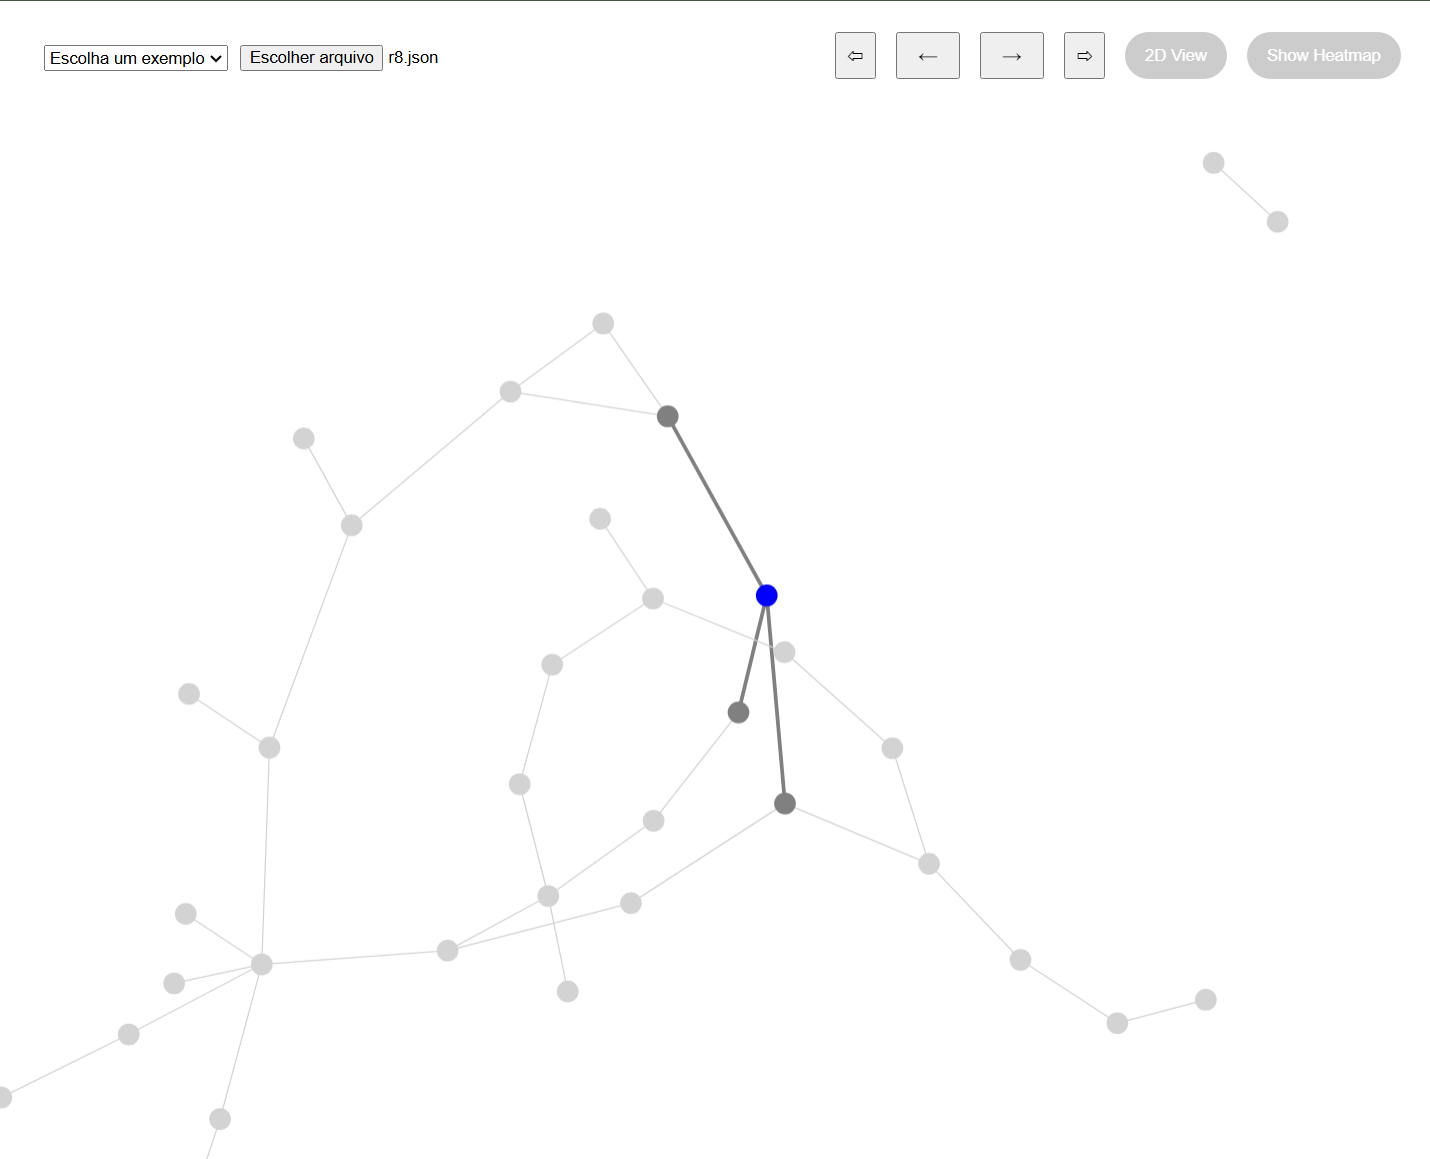
\includegraphics[width=12cm]{GrafoSteps1.png}
\caption{Passo 1 do algoritmo}
\label{fig:grafo-steps-1}
\end{figure}

\begin{figure}[!htb]
\centering
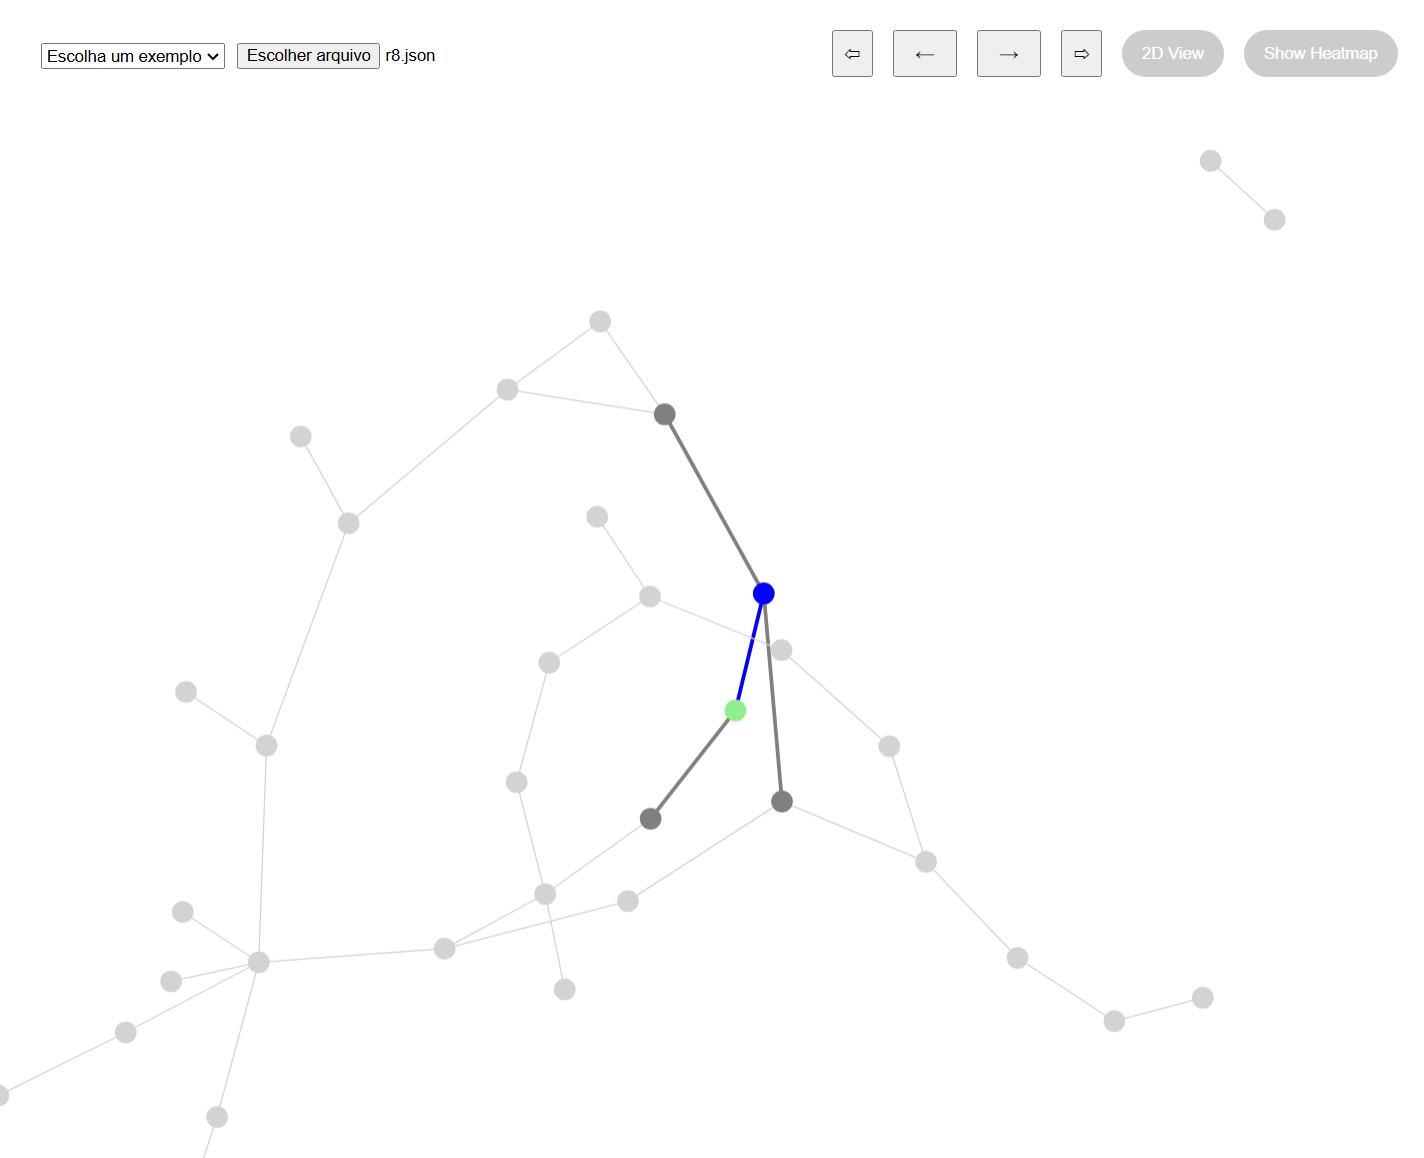
\includegraphics[width=12cm]{GrafoSteps2.png}
\caption{Passo 2 do algoritmo}
\label{fig:grafo-steps-2}
\end{figure}

\begin{figure}[!htb]
\centering
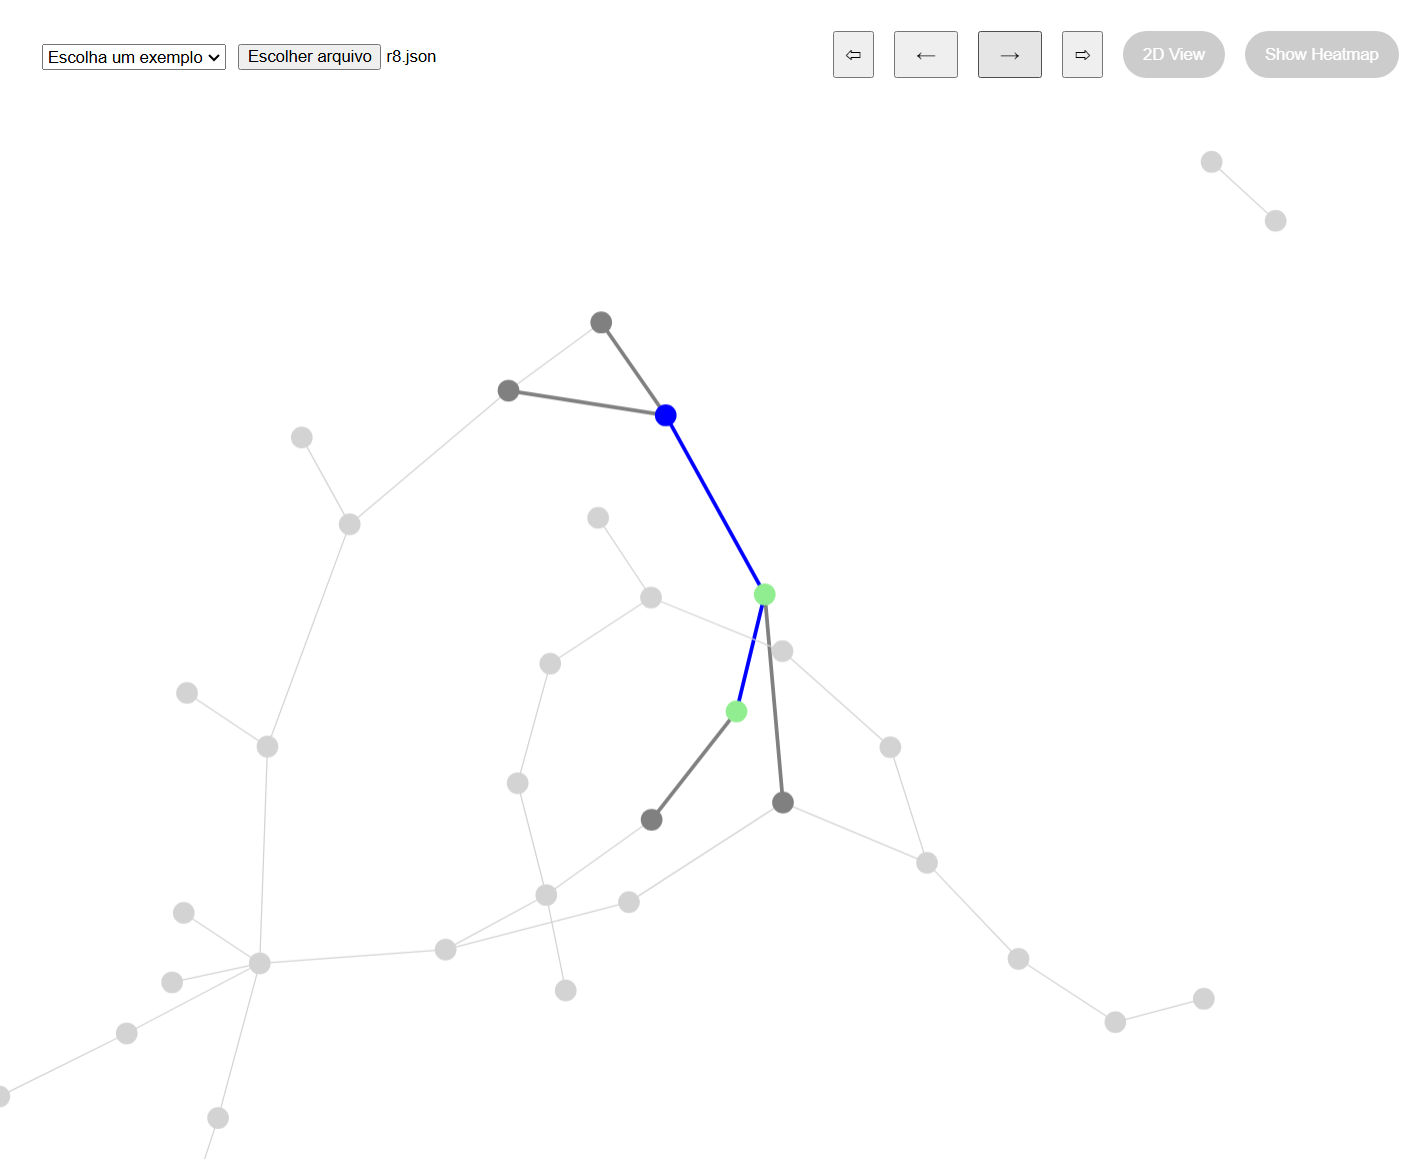
\includegraphics[width=12cm]{GrafoSteps3.png}
\caption{Passo 3 do algoritmo}
\label{fig:grafo-steps-3}
\end{figure}

\begin{figure}[!htb]
\centering
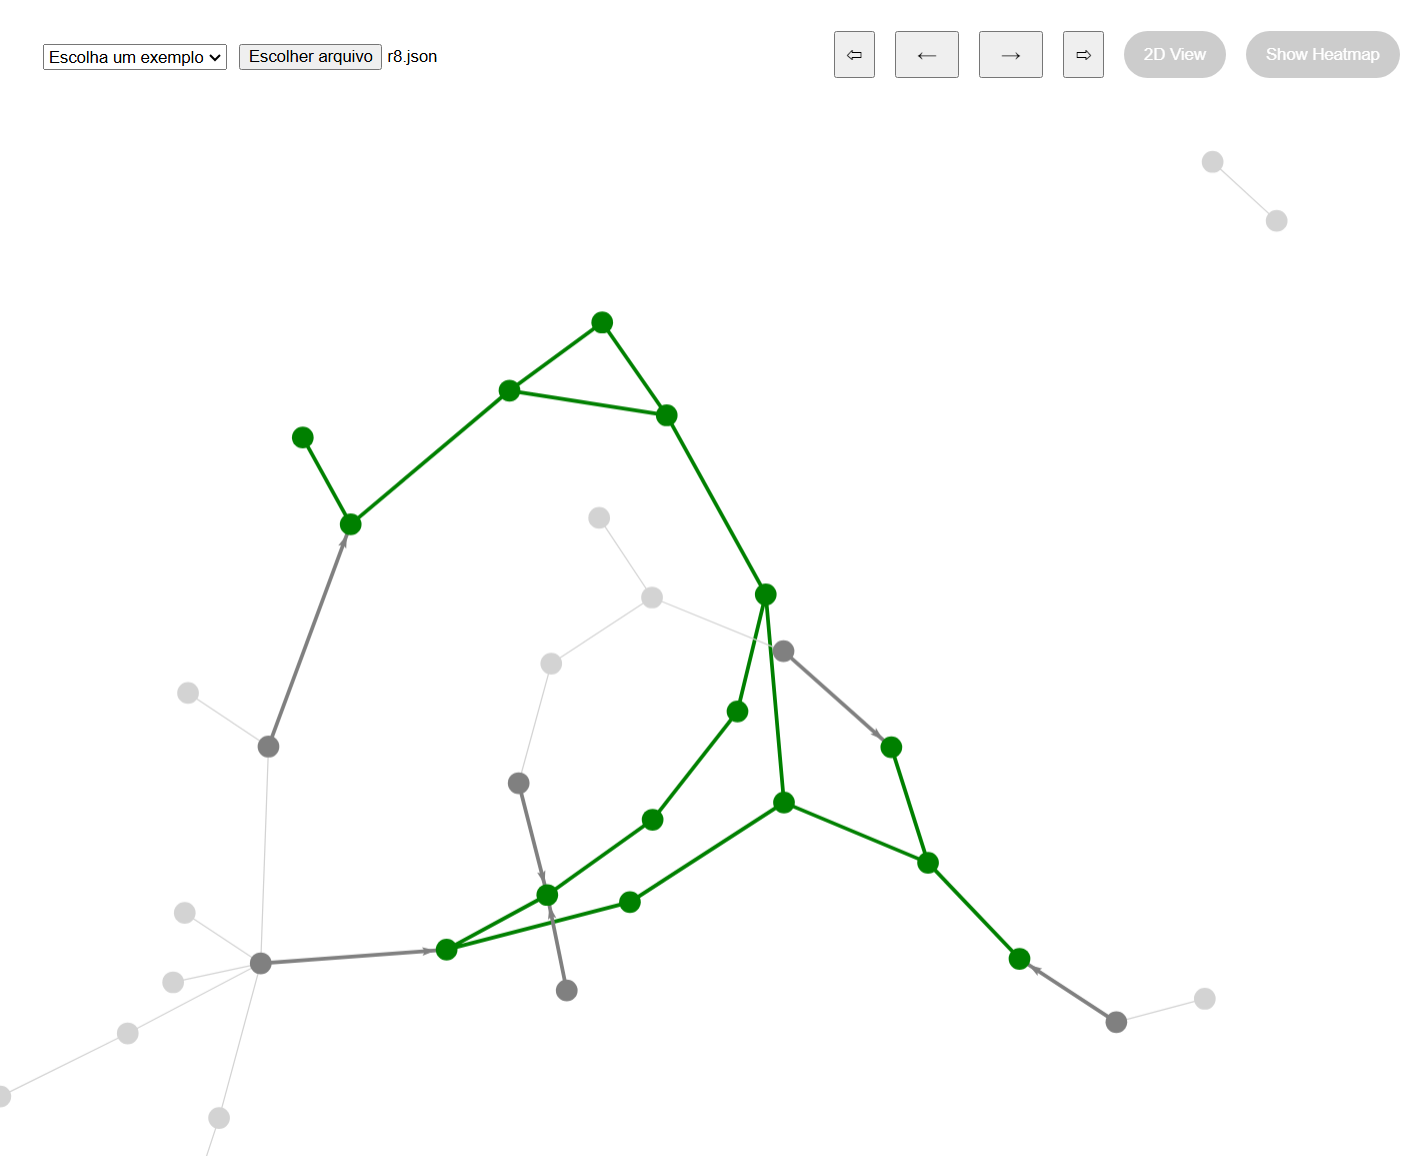
\includegraphics[width=12cm]{GrafoStepsN.png}
\caption{Passo final do algoritmo}
\label{fig:grafo-steps-n}
\end{figure}

\subsection{Mapa de calor}
É possível também ativar a visualização do mapa de calor, que colore os vértices de acordo com a quantidade de vezes que ele foi explorado pelo algoritmo.

\begin{figure}[!htb]
\centering
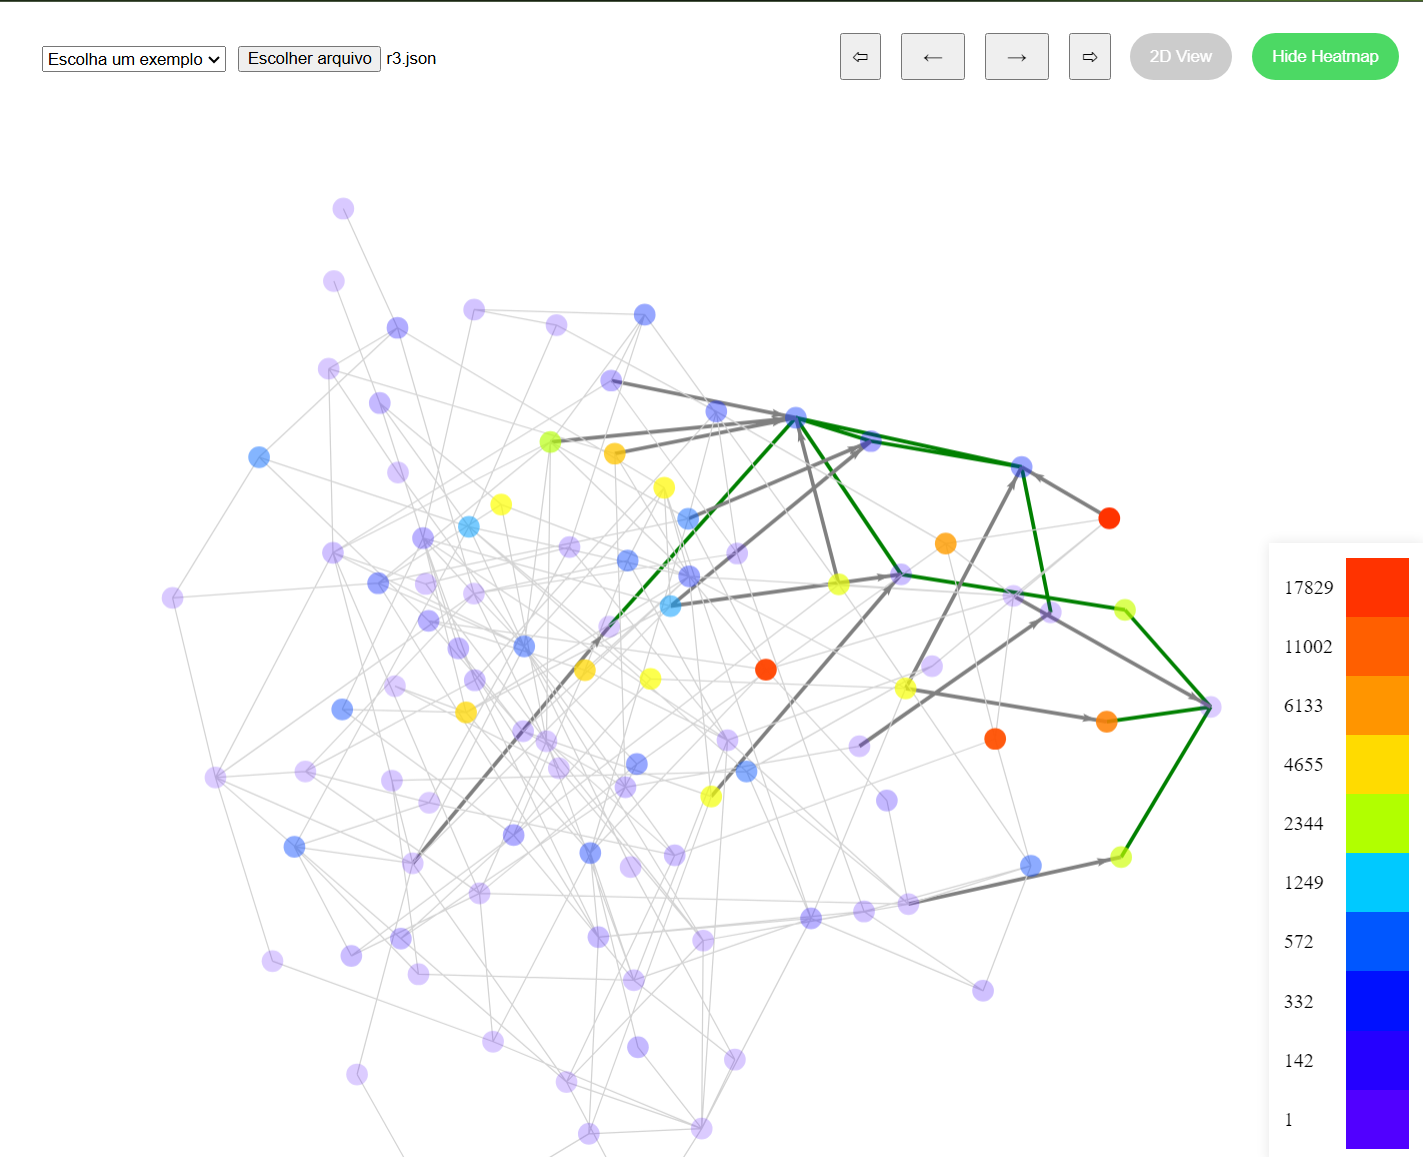
\includegraphics[width=12cm]{GrafoHeatmap.png}
\caption{Mapa de calor do grafo}
\label{fig:grafo-heatmap}
\end{figure}

Para ajudar na visualização, as cores mais frias também tem opacidade mais baixa.

Essa ferramenta em particular incentivou questionamentos interessantes a respeito da eficiência do algoritmo, como "como evitar a alta taxa de repetição de um grupo de vértices".

\chapter{Resultados e discussão}
O algoritmo originalmente estudado e a versão com as melhorias propostas foram analisadas e submetidas a um conjunto de testes para melhor ilustrar o impacto e eficiência de cada uma. Visto que o problema continua sendo NP-completo, há pouco a ser feito para valores realmente grandes, mas foi possível sim observar uma ampliação dos valores considerados "razoáveis" pelo algoritmo FPT.

Para testar o algoritmo utilizamos a função da biblioteca \texttt{networkx nx.erdos\_renyi\_graph(v,e,seed)} onde \texttt{v} é o número de vértices \texttt{e} é a probabilidade de 2 vértices formarem uma aresta, e \texttt{seed} é uma semente para geração do Grafo.

Para os testes a seguir foram fixados os seguintes seguintes parâmetros \texttt{v=30} \texttt{e=0.333} e \texttt{seed=100} e executamos para \texttt{k} variando entre \texttt{1} e \texttt{29}.

\begin{figure}[!htb]
\centering
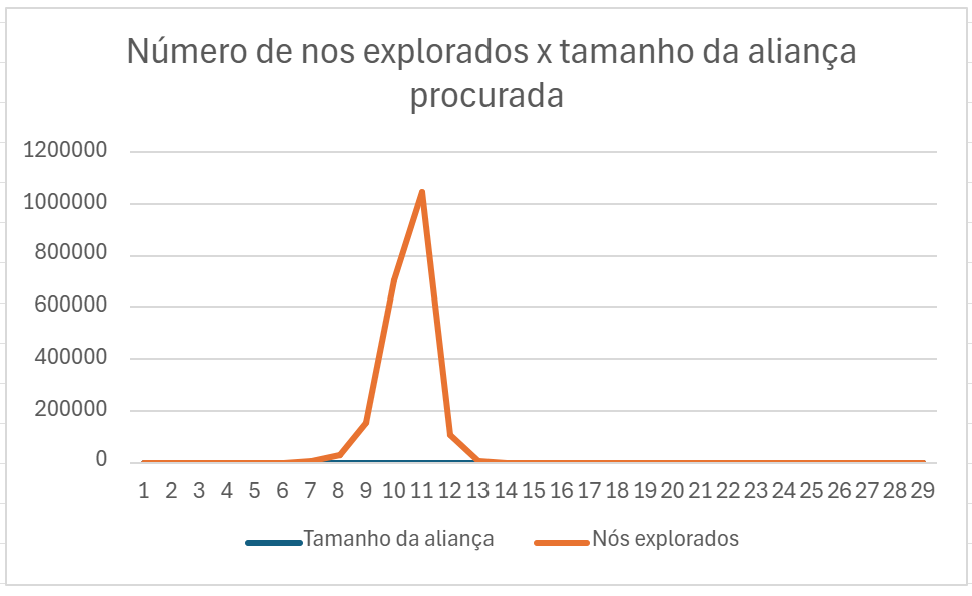
\includegraphics[width=12cm]{Execução sem repetição de conjuntos.png}
\caption{Execução do algoritmo \textbf{evitando} a repetição de conjuntos}
\label{fig:execucao-sem-repeticao}
\end{figure}

Na execução do algoritmo sem repetição de conjuntos é possível notar que o número máximo de nós explorados foi de aproximadamente 1 milhão de nós.

\begin{figure}[!htb]
\centering
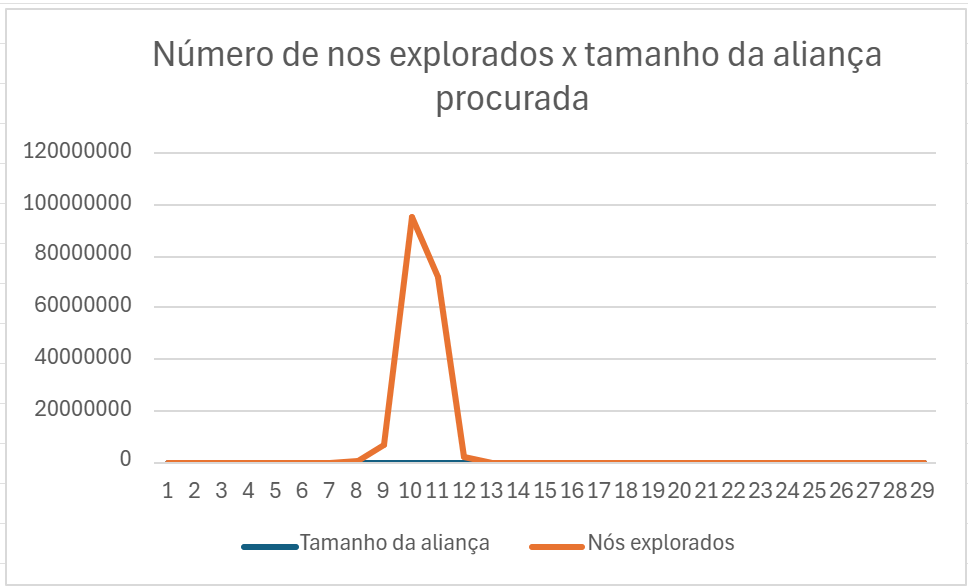
\includegraphics[width=12cm]{Execução com repetição de conjuntos.png}
\caption{Execução do algoritmo \textbf{permitindo} a repetição de conjuntos}
\label{fig:execucao-com-repeticao}
\end{figure}

Por sua vez, na execução que permite a repetição de conjuntos o número de nós explorados nesse caso saltou de 1 milhão para 100 milhões.

Salvar os conjuntos resulta em uma melhora significativa na redução do número de nós a serem explorados, porém nós traz um novo problema pois o espaço necessário para armazenar todos esses conjuntos no pior caso é $\sum_{i=0}^{k} \binom{n}{i}<2^n$, ou seja, acabamos trocando um tempo exponencial, por espaço exponencial.

Foi observado um padrão interessante na eficiência com relação ao grau médio dos vértices do grafo $d(G)$ e $k$; o número de nós explorados atinge um ápice para valores de $k$ próximos de $d(G)$ criando uma "zona difícil", e suaviza a medida que a diferença aumenta.

Para valores de $d(G)$ muito maiores que $k$ isso acontece porque o algoritmo pode descartar muitas combinações através do critério \texttt{Se v.c\_w <= k - tamanho de S:}. Essa linha garante que o próximo nó a ser expandido ao menos tem as condições de ser protegido dado o tamanho atual de $S$.

Por outro lado, valores de $k$ muito menores do que $d(G)$, foi observado uma probabilidade maior de haver uma aliança defensiva. A modificação de ordenação dos vértices de \texttt{W} com base em quantos vizinhos ele possui em $S$ e $\lfloor d(v)/2 \rfloor$, em especial, mostrou acelerar muito o processo de determinação da aliança, quando existente. Isso se deve as escolhas priorizarem a defesa dos vértices já em $S$, em prol de adições aleatórias.

Por fim, a modificação de "Evitar repetir conjuntos" mostrou-se acelerar o processo tanto no melhor caso quanto no pior, pois garante que somente novas combinações são testadas.

\chapter{Conclusão}
O estudo como um todo foi bastante produtivo dentro do tema, e possibilitou compreensão significativa do que são e como encontrar alianças defensivas. O visualizador web, como ferramenta didática, foi bastante aproveitado para a compreensão e elaboração das melhorias propostas ao algoritmo.

Também foi produtivo experimentar na prática a complexidade de um problema NP-completo e uma das ferramentas usadas para contornar esse degrau gigantesco na complexidade.

Dentre os diversos temas que podem ser abordados em discussões futuras, destacamos a implementação e análise do algoritmo proposto por \cite{Enciso2009} para encontrar Conjuntos Seguros (\textit{Secure Sets}), que segue uma abordagem FPT semelhante ao de alianças defensivas, e pode ser adaptado para o visualizador web para gerar resultados valiosos.

Outro ponto de possível expansão é o de pré-análise de grafos para a determinação de potencial de uma aliança de tamanho $k$, partindo da análise feita sobre o grau médio e a "zona difícil".
			% estado da arte
%\chapter{Fundamentação teórica}
A fim de seguir de forma devida com a análise do problema e do algoritmo, algumas definições teóricas são requeridas:

\section{Conceitos}

\subsection{Grafo}
Um grafo $G = (V(G), E(G))$ é um par ordenado que consiste de um conjunto de vértices $V(G)$ e um conjunto de arestas $E(G)$.

\subsection{Vértice}
Um vértice $v \in V(G)$ é um elemento básico de um grafo, representando um ponto ou nó na estrutura. O conjunto $V(G)$ é finito e contém todos os vértices do grafo.

\subsection{Aresta}
Uma aresta $e \in E(G)$ é um conjunto de dois vértices de $V(G)$. Em um grafo não direcionado, a aresta $\{u, v\}$ conecta os vértices $u$ e $v$, sem direção. Em grafos direcionados, uma aresta $(u, v)$ conecta $u$ a $v$ com uma orientação de $u$ para $v$.

\subsection{Incidência}
As extremidades de uma aresta são ditas incidentes com a aresta \cite{Bondy2008}, e vice-versa, ou seja, uma aresta $e$ é dita incidente a um vértice $v$ se está aresta se conecta a $v$ em um de seus extremos.

\subsection{Adjacência}
Dois vértices que são incidentes a uma mesma aresta são adjacentes \cite{Bondy2008}, assim como duas arestas que são incidentes a um mesmo vértice, ou seja, um par de vértices distintos $u$ e $v$ são adjacentes se possuem uma aresta que os conectam, da mesma forma que duas arestas distintas $e1$ e $e2$ são adjacentes se são incidentes a um vértice em comum.

\subsection{Vizinhança de um Vértice}
Dois vértices que são incidentes a uma aresta comum, ou seja, dois vértices adjacentes distintos são ditos vizinhos \cite{Bondy2008}. A vizinhança de um vértice $v \in V(G)$, denotada por $N(v)$, é o conjunto de todos os vértices adjacentes a $v$, ou seja, $N(v) = \{ u \in V(G) \mid \{u, v\} \in E(G) \}$ em grafos não direcionados.

\subsection{Grau de um Vértice}
O grau de um vértice $v$ em um grafo não direcionado $G$ é dado por $d(v) = |N(v)|$, ou seja, o número de arestas incidentes a $v$. Neste estudo consideramos apenas grafos não direcionados, portanto o grau de $v$ corresponde ao número de arestas total ligadas a ele.

\subsection{Subgrafo}
Um \textbf{subgrafo} de um grafo $G$ é um grafo $F$ cujos conjuntos de vértices e arestas são subconjuntos dos vértices e arestas de $G$. Formalmente, $F$ é um subgrafo de $G$ se $V(F) \subseteq V(G)$ e $E(F) \subseteq E(G)$, e a função que relaciona vértices e arestas em $F$ é a mesma que em $G$, mas restrita ao conjunto de arestas de $F$. Subgrafos podem ser formados a partir das operações de remoção de vértices e remoção de arestas.\\
Diz-se que $G$ contém $F$ ou que $F$ está contido em $G$, representado como $G \supseteq F$ ou $F \subseteq G$.

\subsection{Conectividade}
Um grafo é \textbf{conexo} se, para toda partição de seu conjunto de vértices em dois conjuntos não vazios $X$ e $Y$, existe uma aresta com uma extremidade em $X$ e a outra extremidade em $Y$, caso contrário, o grafo é desconexo. Em outras palavras, um grafo é desconexo se seu conjunto de vértices pode ser particionado em dois subconjuntos não vazios $X$ e $Y$ de modo que nenhuma aresta tenha uma extremidade em $X$ e outra em $Y$.

\subsection{Aliança Defensiva}
Um subconjunto $S \subseteq V$ é uma aliança defensiva se, para cada vértice $v \in S$, a condição a seguir é satisfeita:   $|N(v) \cap S| \geq |N(v) \setminus S|$.\\
Ou seja, para cada vértice $v$ na aliança $S$, o número de vértices adjacentes a $v$ dentro de $S$ deve ser pelo menos igual ao número de vértices adjacentes a $v$ fora de $S$.\\
Isso indica que os vértices $v$ na aliança devem possuir pelo menos tantos vértices dentro da aliança quanto fora dela.\\
Embora, formalmente, uma aliança não precise ser conexa, note que cada componente conexa de uma aliança é uma aliança por si só. Para fins deste trabalho, toda aliança encontrada deve ser \textbf{conexa}.

\section{Complexidade Computacional}
A complexidade computacional estuda a quantidade de recursos necessários para a execução de algoritmos, especialmente em termos de tempo e espaço. Em ciência da computação, a complexidade computacional é frequentemente representada usando a notação \textit{Big O}, $O(f(n))$, que descreve o crescimento da complexidade como uma função $f(n)$, onde $n$ normalmente é o tamanho da entrada, ou algum outro parâmetro relevante. Alguns exemplos de classificação de complexidade são:

\begin{itemize}
  \item $O(1)$: Constante, o tempo de execução não depende do tamanho da entrada.
  \item $O(n)$: Linear, o tempo de execução cresce proporcionalmente ao tamanho da entrada.
  \item $O(n^k)$: Polinomial, o tempo de execução cresce proporcionalmente com relação a potência $k$ constante do tamanho da entrada. Um exemplo de polinômio muito comum são os quadrados $O(n^2)$.
  \item $O(k^n)$: Exponencial, o tempo de execução cresce de forma exponencial com relação ao tamanho da entrada. No geral, é inviável para grandes entradas.
  \item $O(n!)$ Fatorial, em problemas fatoriais o tempo de execução cresce ainda mais acelerado com relação ao tamanho da entrada do que problemas exponenciais.
\end{itemize}

\subsection{Classes de Complexidade:}
Os problemas de decisão, como os envolvendo alianças, podem ser classificados em certas classes de complexidade que separam o quão viáveis é encontrar ou verificar suas soluções para entradas de larga escala. Estas classes não:

\begin{itemize}
  \item $P$ (Polinomial): Representa a classe de problemas que podem ser resolvidos em tempo polinomial, ou seja, em $O(n^k)$ para algum inteiro $k$. Em ciência da computação, problemas em $P$ são considerados tratáveis.
  \item $NP$ (Tempo polinomial não determinístico): Representa a classe de problemas para os quais, apesar de não sabermos como encontrar solução em tempo polinomial de maneira determinística, dada uma solução, ela pode ser verificada em tempo polinomial por um algoritmo determinístico. Não sabemos se todo problema em $NP$ pode ser resolvido em tempo polinomial, isto é, se $P = NP$, e esse é um dos 7 problemas do milênio que ainda estão em aberto.
  \item $NP$-completo: Representa um subconjunto de problemas em $NP$ que são, intuitivamente, tão difíceis quanto qualquer outro problema em $NP$. Para um problema ser dessa classe, são necessárias duas características:
  \begin{enumerate}
    \item Estar em $NP$, ou seja, dada uma solução, ela deve ser verificável em tempo polinomial.
    \item Ser $NP$-difícil, todo problema em $NP$ pode ser redutível a ele em tempo polinomial.\\
Em outras palavras, caso um problema de classe $NP$-completo seja resolvido em tempo polinomial, todos os outros problemas em $NP$ poderão ser resolvidos em tempo polinomial.
  \end{enumerate}
\end{itemize}

\section{O algoritmo}
Como encontrar uma aliança defensiva em um grafo é um problema NP-completo, o algoritmo FPT \cite{Enciso2009} tem como objetivo buscar por uma aliança conexa arbitrária de tamanho máximo $k$, a fim de tornar o problema tratável. Porém, neste trabalho o tamanho da aliança buscada será \textit{exatamente} $k$, pois acreditamos que o tamanho da aliança seja importante. Antes de entrar na explicação minuciosa do algoritmo, é importante explicar o que é um algoritmo FPT.

\subsection{Complexidade}
FPT (\textit{Fixed-Parameter Tractable}) é uma classe de complexidade que trata de problemas parametrizáveis (como os de complexidade exponencial) ao isolar e fixar um parâmetro específico do problema, chamado $k$, e então expressando a complexidade na forma $f(k)*p(n).$ Desta forma, $f(k)$ é a parte da complexidade que depende exclusivamente de $k$ e pode ser \textit{superpolinomial}, enquanto $p(n)$ é uma função polinomial de $n$. Sendo assim, fixar $k$ em valores pequenos nos permite abordar o algoritmo de forma mais tratável, custando muito menos tempo, a depender do tamanho de $k$.

O algoritmo usado neste estudo foi proposto por \cite{Enciso2009}, e tem complexidade $O(k^kn)$, e é uma melhora significativa de seu predecessor, que tinha complexidade $O((2k-1)^kk^2n)$. Esse é um avanço substancial, mas ainda é interessante demonstrar como problemas, mesmo parametrizados, crescem rapidamente:

\begin{table}[h]
\begin{center}
\begin{tabular}{|c|c|c|c|c|c|c|c|}
\hline
$k$ & $k^k$\\
\hline
2 & 4 \\
\hline
3 & 27 \\
\hline
4 & 256 \\
\hline
5 & 3.125 \\
\hline
6 & 46.656 \\
\hline
7 & 823.543 \\
\hline
9 & 387.420.489 \\
\hline
10 & 10.000.000.000 \\
\hline
\end{tabular}
\end{center}
\end{table}

\begin{figure}[!htb]
\centering
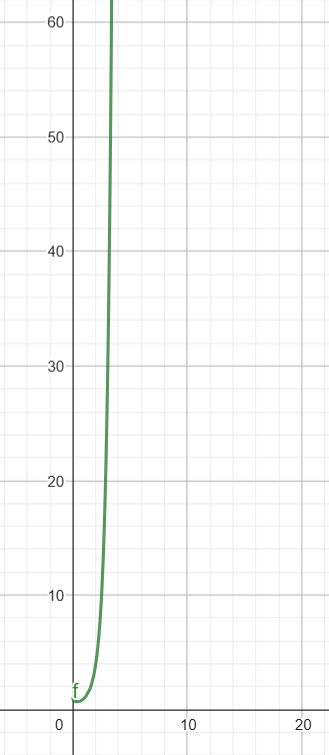
\includegraphics[height=12cm]{GraficoKelevK.png}
\caption{Gráfico da função $k^k$}
\label{fig:kelevk}
\end{figure}

O propósito do algoritmo então é garantir que o tempo possa ser diminuído de acordo com $k$, sem que seja necessário executar para todo $n-k$ restante.

\subsection{Explicação}
O algoritmo é dividido em duas funções principais, a \texttt{main} e a \texttt{defensiveAlliance}. A \texttt{main} recebe como entrada um Grafo $G$ e o tamanho da aliança desejada, um inteiro positivo $k$. De forma intuitiva, a abordagem do algoritmo é partir de um vértice do grafo por vez e olhar sua vizinhança numa tentativa de expandi-lo até formar uma aliança defensiva de tamanho $k$, ou todos os vértices terem servido de raiz da expansão.

\lstset{ 
  deletekeywords={do}  
}

\begin{lstlisting}[escapeinside={(*}{*)}]
Main(G,k)
	Para cada vértice v de G:
		v.c_w <- (*$\ceil{\frac{d(v)}{2}}$*).
	Para cada vértice v de G:
		inicia uma aliança S <- {v}.
		aliança_encontrada <- DefensiveAlliance(S).
		Se aliança_encontrada:
			retorne aliança_encontrada.
		retira v de S
		soma 1 ao c_w de v.
			
	retorne "Sem aliança";
\end{lstlisting}

O papel da função \texttt{main} é garantir que todos os vértices foram usados como raiz da expansão. Para isso, primeiro é definido o \texttt{c\_w}, que serve para verificar se o vértice está protegido dentro da aliança \texttt{S}. De início, ela é definida com o número de vizinhos necessários dentro de $S$ para que ele esteja defendido, e então será aumentada ou diminuida conforme se adiciona ou remove seus vizinhos a $S$.

Isso também faz parte da condição de sucesso da busca, ou seja, quando todos os vértices de \texttt{S} estiverem protegidos (\texttt{c\_w <= 0}) então uma aliança defensiva foi formada.

A seguir, a \texttt{main} chama a função \texttt{defensiveAlliance} para verificar se \texttt{S} é, ou pode ser expandida até, uma aliança defensiva de tamanho \texttt{k}.

\begin{lstlisting}[escapeinside={(*}{*)}]
DefensiveAlliance(G, S, k)
	inicia v <- vértice de maior c_w em S.
	Se v.c_w <= 0 e tamanho de S == k:
		devolve S.
		
	Se v.c_w <= k - tamanho de S: 
		inicia t <- 1 + metade dos vizinhos de w.
		inicia o conjunto W <- t vizinhos de w que não pertencem a S.
		Para cada vértice w em W:
			S <- S + w.
			Para cada vizinho x de w em S:
				subtrai 1 do c_w de x e de w.
			aliança_encontrada <- DefensiveAlliance(G, S, k)
			Se aliança_encontrada:
				Devolve aliança_encontrada.
			Para cada vizinho x de w em S:
				soma 1 ao c_w de x e de w.
			Retira w de S.
			
	Retorne NULL;
\end{lstlisting}

No início de \texttt{defensiveAlliance} o algoritmo escolhe o vértice de maior \texttt{c\_w} em \texttt{S},  que seria o vértice mais vulnerável da aliança. Esse vértice serve para tanto verificar se \texttt{S} se tornou uma aliança quanto como ponto de expansão a fim de incluir novos vértices.

A seguir, o algoritmo verifica se há espaço em \texttt{S} para os \texttt{c\_w} vizinhos necessários serem adicionados, ou seja, para que \texttt{w} seja defendido dentro da restrição do tamanho máximo \texttt{k}. Essa verificação funciona de modo semelhante a uma heurística de busca, poupando tempo ao evitar vértices que não podem ser defendidos posteriormente.

\subsection{Lema 14}
Uma parte importante do funcionamento do algoritmo é o lema 14 de \cite{Enciso2009}. Assuma que $S \subseteq V$ é estendível para uma aliança defensiva S', onde $|S| <|S'| = k$ então, para qualquer vértice desprotegido $w \in S$, $|S' \cap (N[w] - S|) \ge c_w$.\\
Em outras palavras se $S$ é estendível e $w$ é um vértice desprotegido de $S$ então $c_w$ é o número de vizinhos de $w$ fora de $S$ que é necessário para proteger $w$ em $S$.

Esse lema é o que podemos considerar como o núcleo do algoritmo, pois ele nos garante também que para qualquer subconjunto $W \subseteq N[w] - S$ com $t = \lfloor \frac{d_w}{2} \rfloor + 1$  vértices contém ao menos um vértice $w_i$ para o qual $S \cup {w_i}$ é estendível se e somente se S é estendível.

\subsection{Evitando repetir conjuntos}
Observando o comportamento do algoritmo no visualizador web foi possível notar que um comportamento pouco eficiente: o critério de expansão de $S$ (destacado a seguir) abre margem pra repetir várias vezes a mesma combinação de vértices, levando, principalmente em grafos de grande quantidade de vértices, a muito esforço improdutivo.

\begin{lstlisting}
DefensiveAlliance(G, S, k)
	inicia v <- vértice de maior c_w em S.
\end{lstlisting}

Pensando nisso a equipe elaborou uma solução que armazena todas as combinações já analisadas anteriormente e impede de que novas iterações com elas sejam geradas, cortando toda a sub-árvore subsequente. Isso é feito com a criação de um dicionário e a marcação única de cada combinação:

\begin{lstlisting}
inicia combinacoes <- dicionário vazio
\end{lstlisting}

\begin{lstlisting}
DefensiveAlliance(G, S, k)
[...]
	Para cada vértice w em W:
		S <- S + w.
		
		comb_id <- identificadores de S de forma ordenada.
		Se existe combinacoes[comb_id]:
			Retira w de S.
			pula para o próximo vértice.
		Caso contrário:	
			cria combinacoes[comb_id].

		Para cada vizinho x de w em S:
			subtrai 1 do c_w de x e de w.
		aliança_encontrada <- DefensiveAlliance(G, S, k)
[...]
\end{lstlisting}

Caso não exista uma entrada da combinação no dicionário, cria-se uma e a instância corrente de \texttt{S} é analisada. Caso contrário, a instância é ignorada, podando todas as sub-árvores subsequentes. A complexidade de tempo é se resume a ordenação de, no máximo, $k-1$ elementos, e ao acesso e escrita no dicionário. Ambos são ofuscados pela complexidade geral.

Por outro lado, há um custo sério em termos de espaço. No pior caso, de não haver aliança e o algoritmo analisar todos os vértices e $k=n$, a combinação ocupa espaço $O(2^n)$, que corresponde a guardar todas as combinações de $n$ vértices, variando de tamanho $1$ até $n$. Isso pode ser mitigado ao limitar o tamanho das combinações armazenadas para a região crítica que vai ser repetida mais vezes. A análise desta região está na seção sobre Resultados e discussão.

Quanto ao desempenho, esta técnica permite ao algoritmo poupar muito tempo ao "amortizar" o custo $k^k$ ao longo de várias iterações, pois, como nenhuma combinação é repetida, quanto mais exploradas são as combinações dos vértices, menos combinações existem para serem analisadas.

\subsection{Priorização dos vértices expostos}
\begin{lstlisting}
DefensiveAlliance(G, S, k)
	inicia v <- vértice de maior c_w em S.
\end{lstlisting}

Ao iniciarmos $DefensiveAlliance(G,S,k)$ atribuindo $v$ o vértice em $W$ com maior $c_w$ nós garantimos que a maior prioridade em cada chamada recursiva da função é proteger o vértice mais "exposto".

Assim obtemos também um critério de parada consistente, ou seja, quando o vértice com maior $c_w$ ter $c_w \le 0$ e $|S| = k$, teremos duas informações fundamentais sobre o contexto da execução:\\
1 - Se $c_w \le 0$, então todos os vértices em $S$ estão protegidos.\\
2 - Se $|S|=k$, encontramos a aliança defensiva procurada.

\chapter{Metodologia}
O projeto é composto por duas partes principais: algoritmos de busca implementados em Python e um visualizador web criado para exibir os passos deste algoritmo. As partes funcionam de forma independente, sendo conectadas apenas pelo formato de entrada e saída dos programas.

\section{Algoritmo em Python}
A implementação do algoritmo proposto por \cite{Enciso2009} foi feita em Python e consta completa no Apêndice 1.

Nesta implementação foi utilizada a estrutura de dados da biblioteca \textit{Networkx} para manipulação dos grafos, e, no mais, estruturada de forma semelhante ao algoritmo teórico, com a exceção do uso de uma estrutura de pilha para substituir a chamada recursiva.

Além do resultado final, o programa possibilita o retorno da aliança em formato JSON, com as características utilizadas no visualizador web. Essas características permitem a visualização passo a passo dos nós expandidos pelo algoritmo, e consistem do conjunto $W$ a cada iteração da função \texttt{DefensiveAlliance}.

Há também \textit{flags} para mostrar a quantidade de nós expandidos, para gerar um grafo aleatório segundo uma densidade especificada, e para alterar o comportamento da busca, como retornar a primeira aliança encontrada independente do tamanho.

\section{Visualizador web}
O projeto web foi desenvolvido com Typescript e React, e sua proposta é fornecer uma visualização passo-a-passo do algoritmo e do grafo de entrada. Assim como o algoritmo de busca, o visualizador pode ser encontrado no repositório que se encontra nas referências.

Para montar a visualização é necessário que seja fornecido como entrada um grafo disposto em formato JSON, contando com dois conjuntos extras de dados que são a aliança encontrada, caso exista, e um vetor de \textit{steps}, que contém o conjunto $W$ no dado \textit{passo} da iteração.

Munido destas informações, o visualizador organiza os dados internamente para melhorar o desempenho e a decisão de cada caraterística visual do grafo e então personaliza uma \textit{view} HTML, dada pela biblioteca 3d-force-graph \cite{HassanShafique2004}, que cuida da renderização e simulação física do grafo.

Dentre as funcionalidades, vale destacar duas principais: a visualização do conjunto $S$ a cada etapa do algoritmo e o mapa de calor dos nós explorados. O mapa de calor é a coloração dos vértices do grafo seguindo a regra de que, quanto mais visitado um vértice durante a execução do algoritmo, mais quente é a cor usada; os nós mais quentes tem cores próximas do vermelho, e os mais frios, mais próximas do azul.

\subsection{Visualização por passos}
Ao carregar um grafo com o conjunto de passos, é possível navegar por cada um deles. Em um certo passo, os vértices e arestas da fronteira de $S$ são desenhados com uma cor cinza escura, os além da fronteira tem cor cinza claro, e os vértices dentro de $S$ ficam coloridos com a cor

\begin{itemize}
  \item azul, se estiverem desprotegidos;
  \item ou verde, se estiverem devidamente protegidos.
\end{itemize}

Ao finalizar o algoritmo e desenhar a aliança, ela é colorida de verde escuro.

As figuras a seguir são de uma busca por uma aliança de tamanho $k = 15$ em um grafo de $v=50$ vértices e $e=40$ arestas. O algoritmo começa com $S$ contendo o vértice colorido de azul.

\begin{figure}[!htb]
\centering
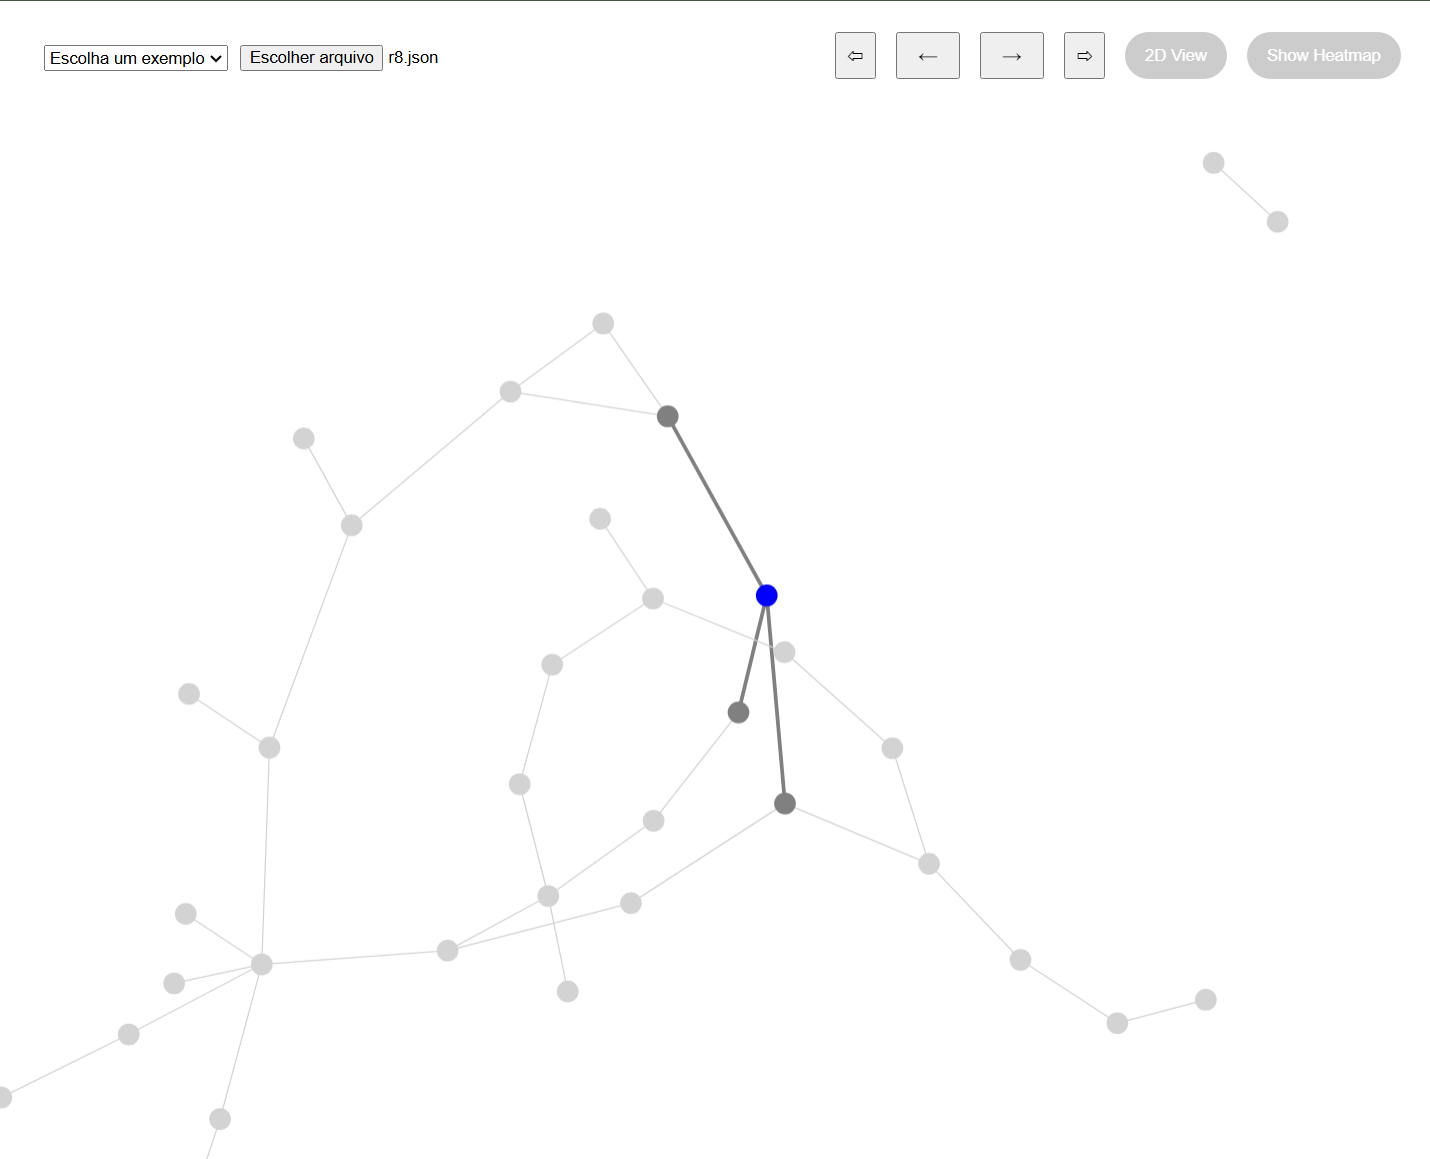
\includegraphics[width=12cm]{GrafoSteps1.png}
\caption{Passo 1 do algoritmo}
\label{fig:grafo-steps-1}
\end{figure}

\begin{figure}[!htb]
\centering
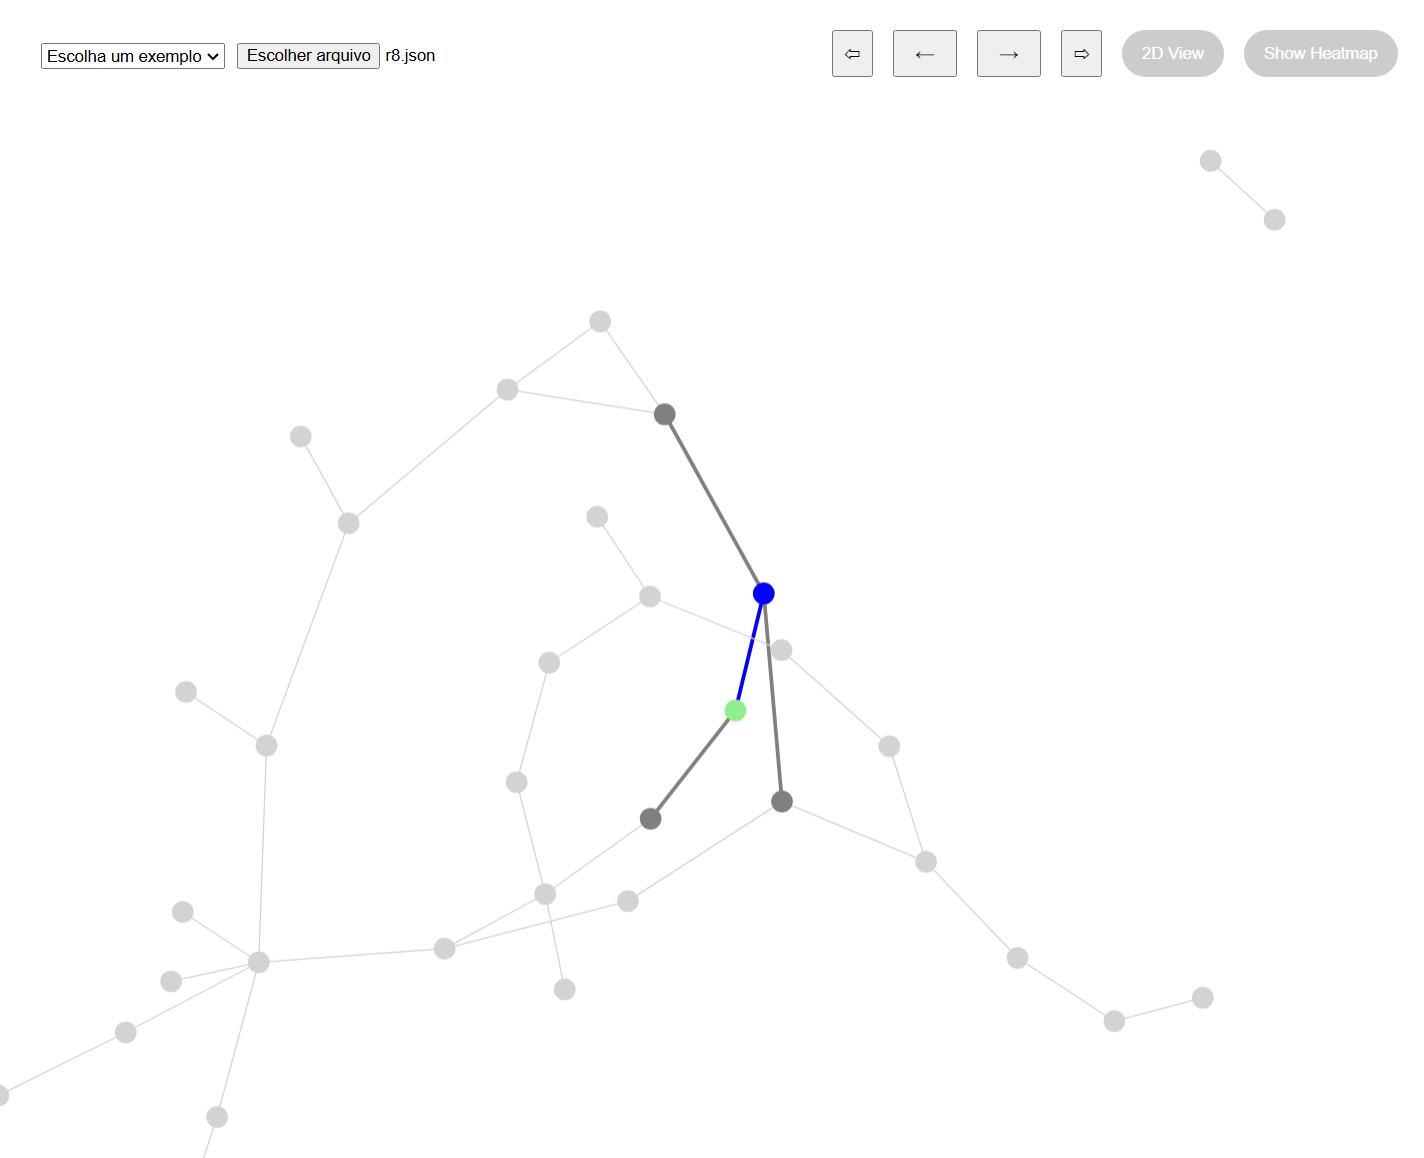
\includegraphics[width=12cm]{GrafoSteps2.png}
\caption{Passo 2 do algoritmo}
\label{fig:grafo-steps-2}
\end{figure}

\begin{figure}[!htb]
\centering
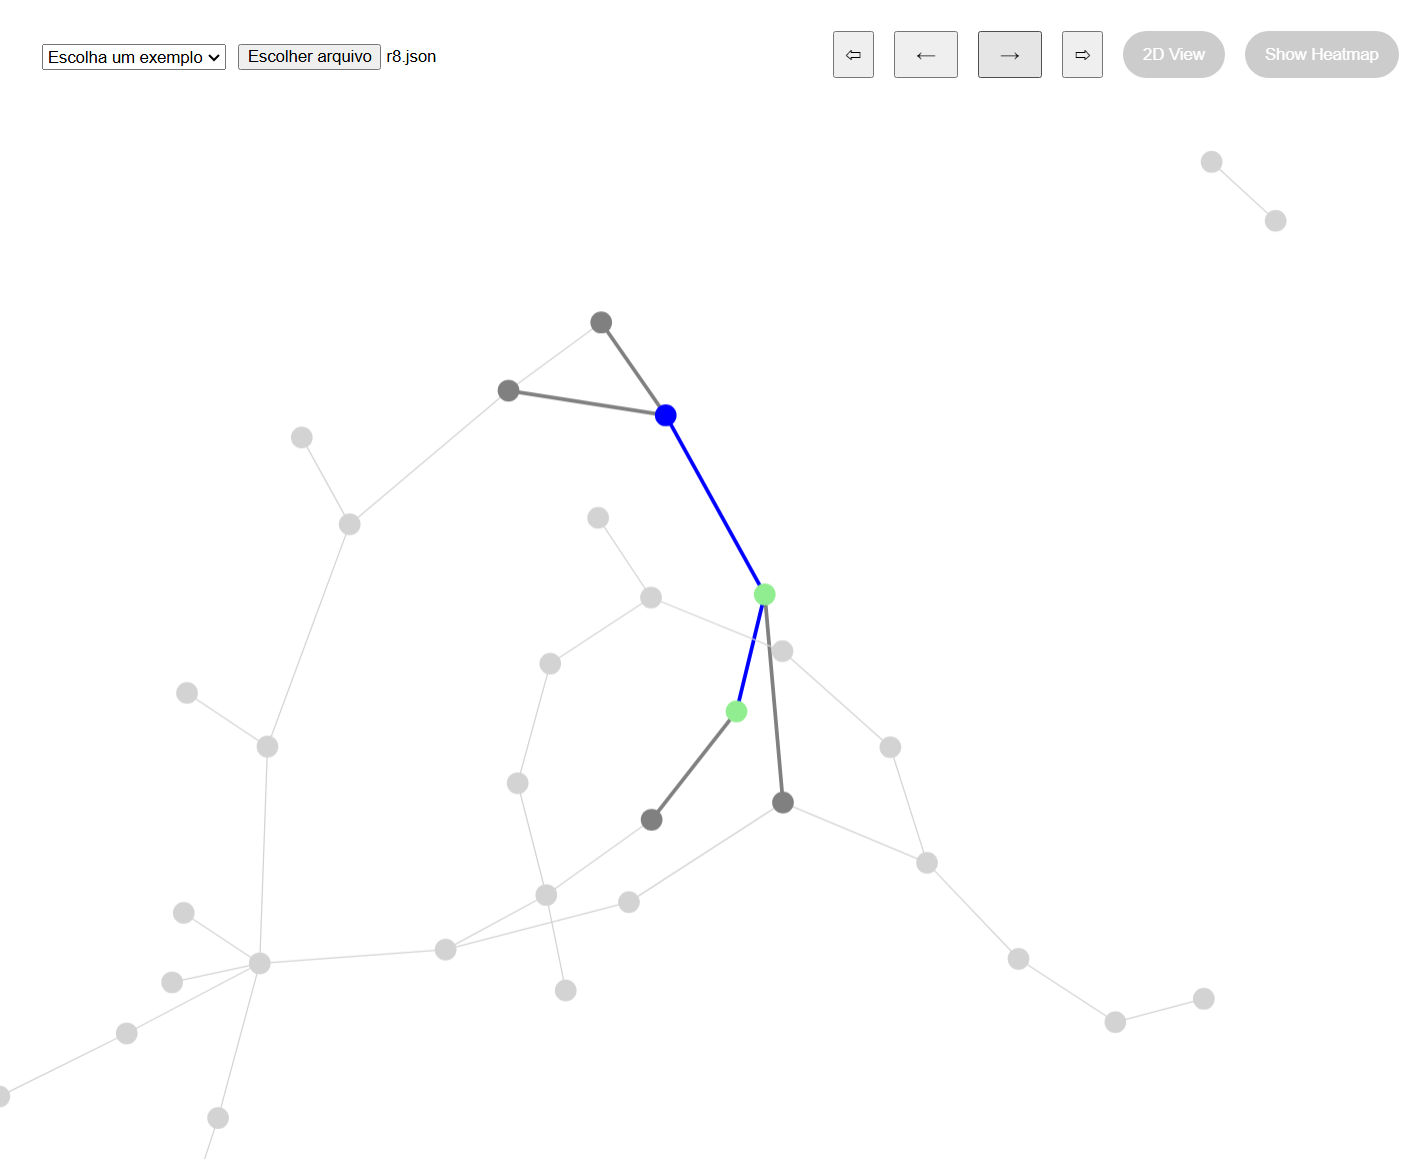
\includegraphics[width=12cm]{GrafoSteps3.png}
\caption{Passo 3 do algoritmo}
\label{fig:grafo-steps-3}
\end{figure}

\begin{figure}[!htb]
\centering
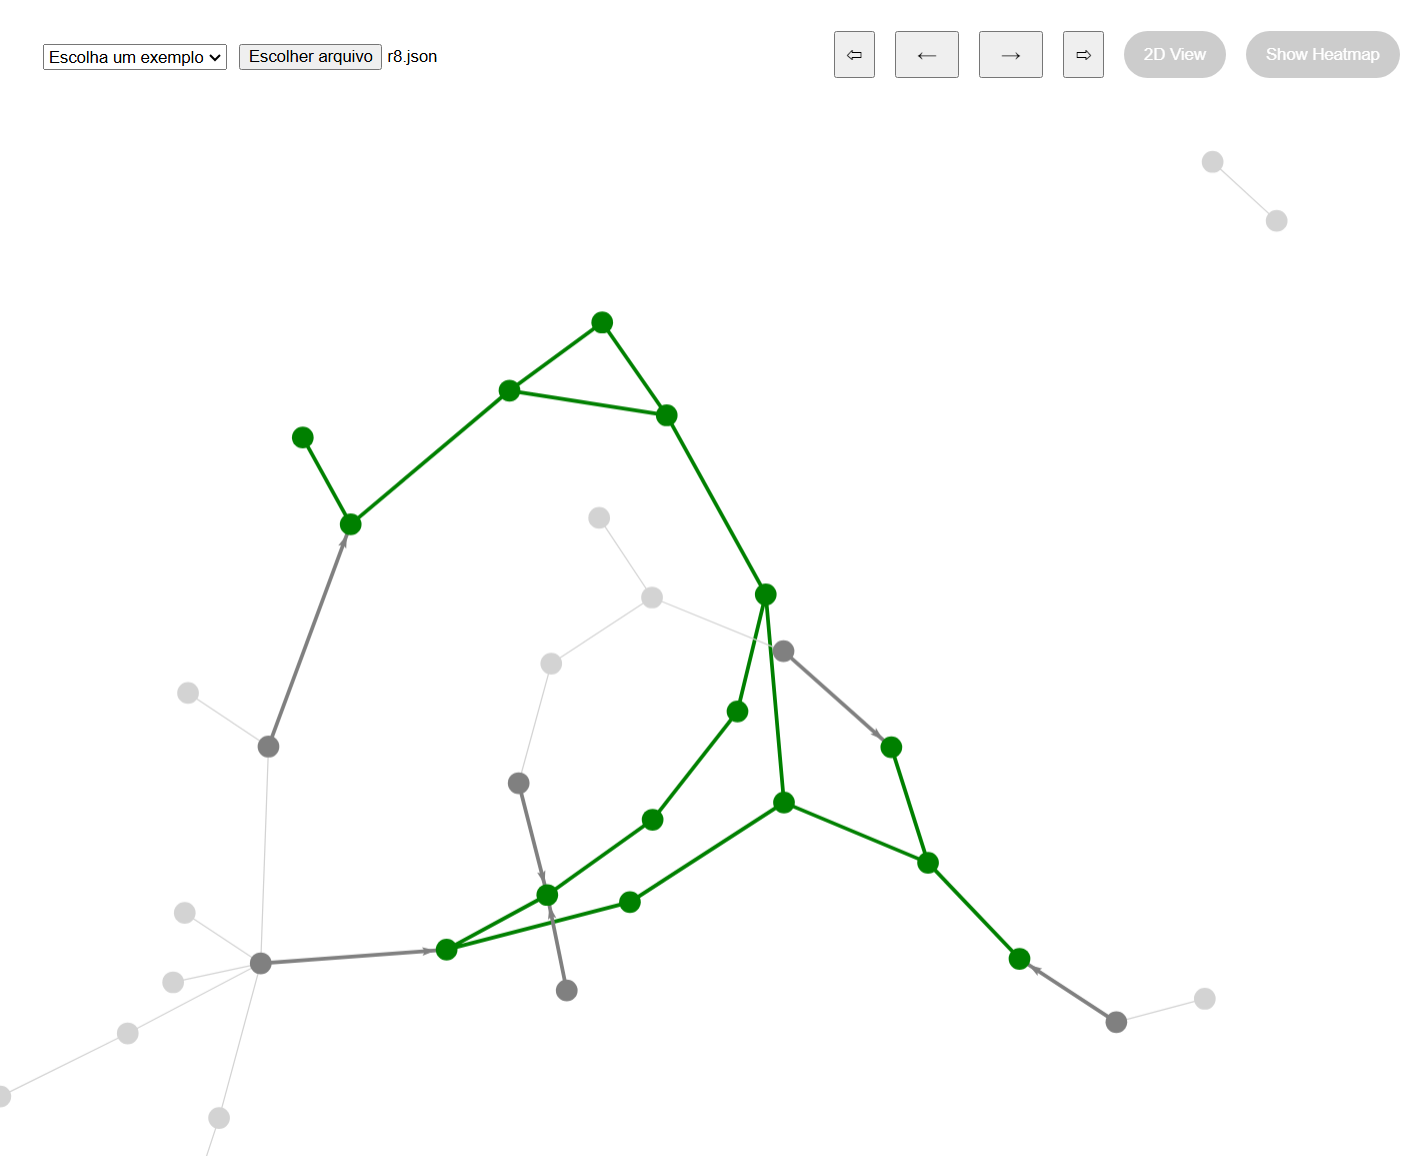
\includegraphics[width=12cm]{GrafoStepsN.png}
\caption{Passo final do algoritmo}
\label{fig:grafo-steps-n}
\end{figure}

\subsection{Mapa de calor}
É possível também ativar a visualização do mapa de calor, que colore os vértices de acordo com a quantidade de vezes que ele foi explorado pelo algoritmo.

\begin{figure}[!htb]
\centering
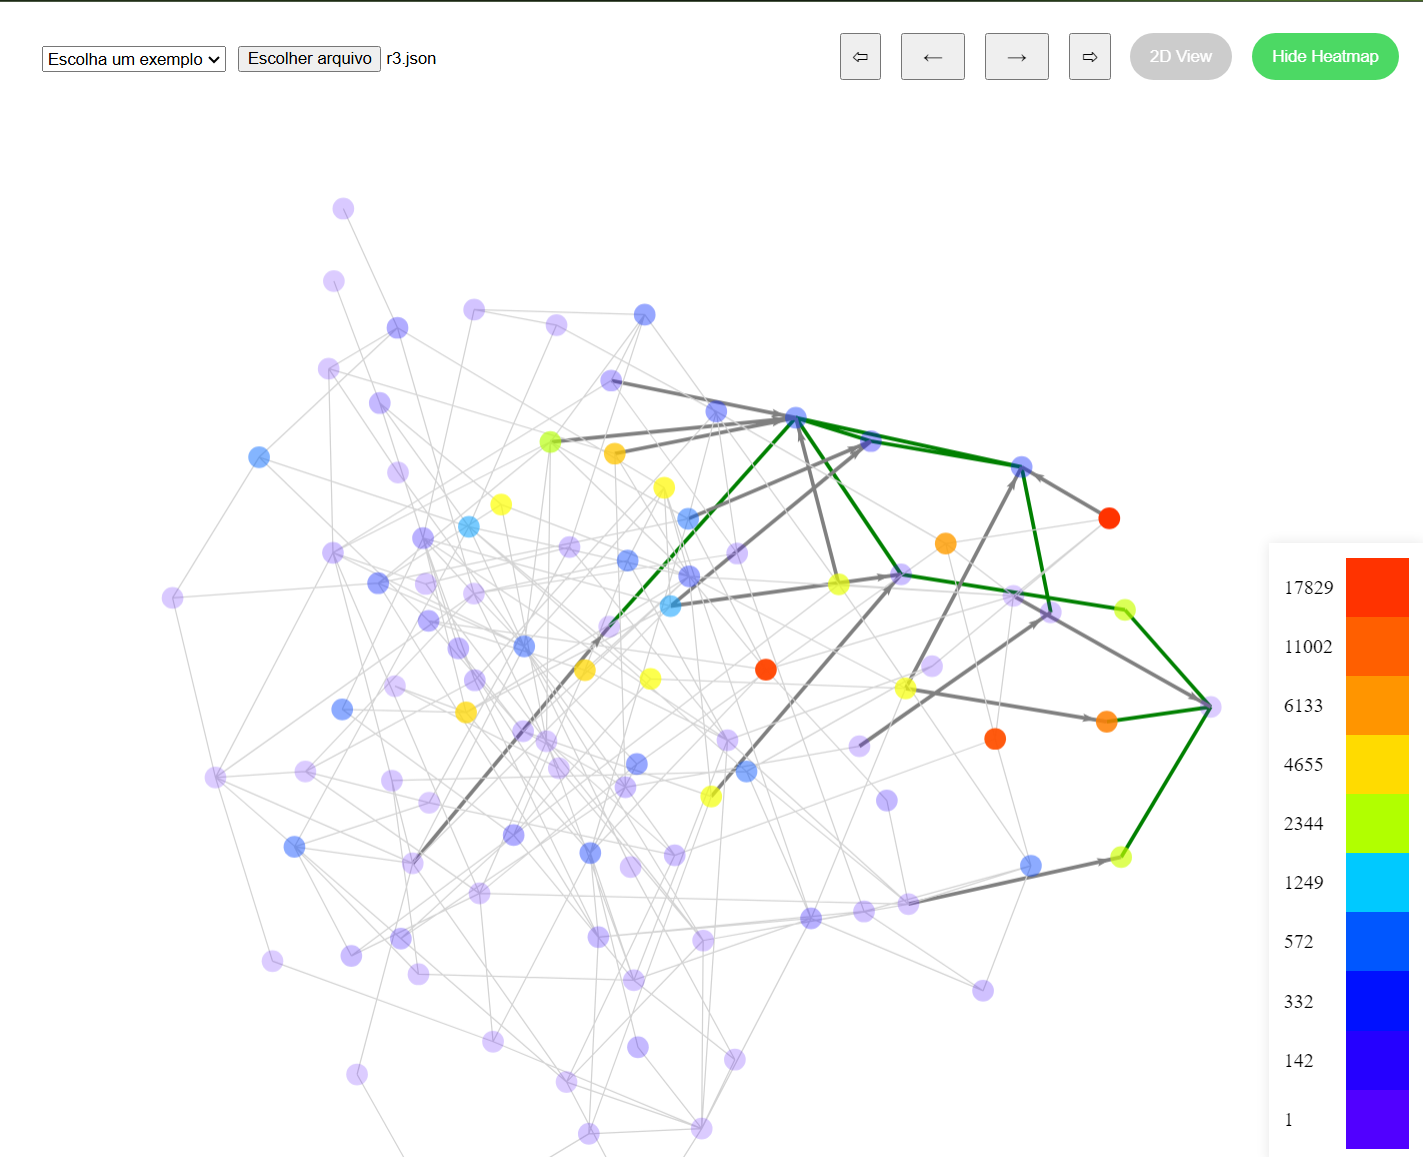
\includegraphics[width=12cm]{GrafoHeatmap.png}
\caption{Mapa de calor do grafo}
\label{fig:grafo-heatmap}
\end{figure}

Para ajudar na visualização, as cores mais frias também tem opacidade mais baixa.

Essa ferramenta em particular incentivou questionamentos interessantes a respeito da eficiência do algoritmo, como "como evitar a alta taxa de repetição de um grupo de vértices".

\chapter{Resultados e discussão}
O algoritmo originalmente estudado e a versão com as melhorias propostas foram analisadas e submetidas a um conjunto de testes para melhor ilustrar o impacto e eficiência de cada uma. Visto que o problema continua sendo NP-completo, há pouco a ser feito para valores realmente grandes, mas foi possível sim observar uma ampliação dos valores considerados "razoáveis" pelo algoritmo FPT.

Para testar o algoritmo utilizamos a função da biblioteca \texttt{networkx nx.erdos\_renyi\_graph(v,e,seed)} onde \texttt{v} é o número de vértices \texttt{e} é a probabilidade de 2 vértices formarem uma aresta, e \texttt{seed} é uma semente para geração do Grafo.

Para os testes a seguir foram fixados os seguintes seguintes parâmetros \texttt{v=30} \texttt{e=0.333} e \texttt{seed=100} e executamos para \texttt{k} variando entre \texttt{1} e \texttt{29}.

\begin{figure}[!htb]
\centering
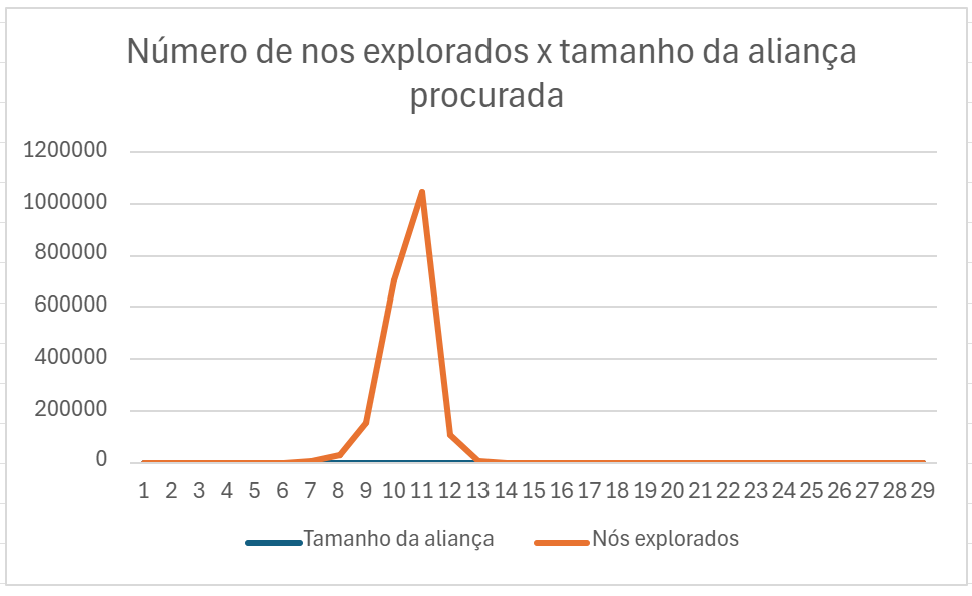
\includegraphics[width=12cm]{Execução sem repetição de conjuntos.png}
\caption{Execução do algoritmo \textbf{evitando} a repetição de conjuntos}
\label{fig:execucao-sem-repeticao}
\end{figure}

Na execução do algoritmo sem repetição de conjuntos é possível notar que o número máximo de nós explorados foi de aproximadamente 1 milhão de nós.

\begin{figure}[!htb]
\centering
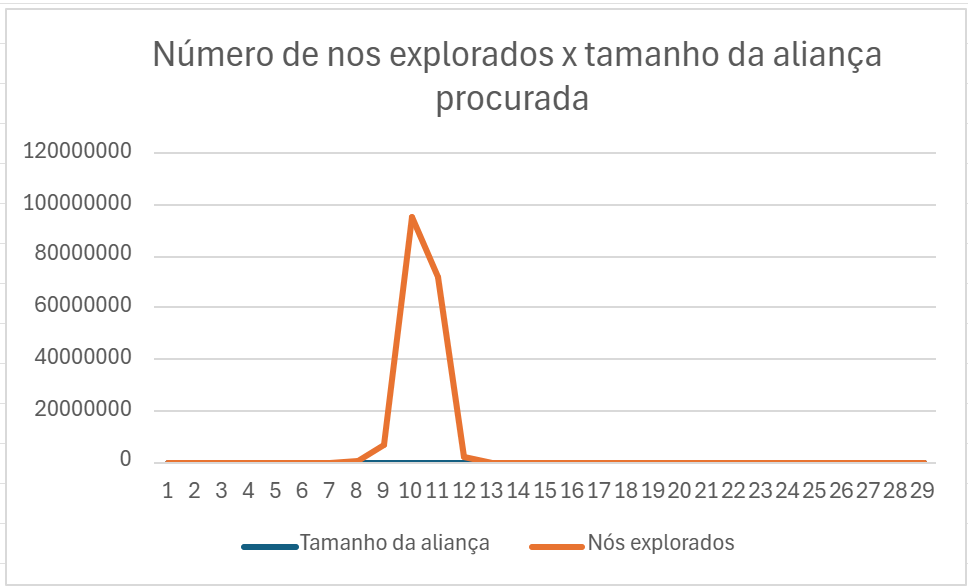
\includegraphics[width=12cm]{Execução com repetição de conjuntos.png}
\caption{Execução do algoritmo \textbf{permitindo} a repetição de conjuntos}
\label{fig:execucao-com-repeticao}
\end{figure}

Por sua vez, na execução que permite a repetição de conjuntos o número de nós explorados nesse caso saltou de 1 milhão para 100 milhões.

Salvar os conjuntos resulta em uma melhora significativa na redução do número de nós a serem explorados, porém nós traz um novo problema pois o espaço necessário para armazenar todos esses conjuntos no pior caso é $\sum_{i=0}^{k} \binom{n}{i}<2^n$, ou seja, acabamos trocando um tempo exponencial, por espaço exponencial.

Foi observado um padrão interessante na eficiência com relação ao grau médio dos vértices do grafo $d(G)$ e $k$; o número de nós explorados atinge um ápice para valores de $k$ próximos de $d(G)$ criando uma "zona difícil", e suaviza a medida que a diferença aumenta.

Para valores de $d(G)$ muito maiores que $k$ isso acontece porque o algoritmo pode descartar muitas combinações através do critério \texttt{Se v.c\_w <= k - tamanho de S:}. Essa linha garante que o próximo nó a ser expandido ao menos tem as condições de ser protegido dado o tamanho atual de $S$.

Por outro lado, valores de $k$ muito menores do que $d(G)$, foi observado uma probabilidade maior de haver uma aliança defensiva. A modificação de ordenação dos vértices de \texttt{W} com base em quantos vizinhos ele possui em $S$ e $\lfloor d(v)/2 \rfloor$, em especial, mostrou acelerar muito o processo de determinação da aliança, quando existente. Isso se deve as escolhas priorizarem a defesa dos vértices já em $S$, em prol de adições aleatórias.

Por fim, a modificação de "Evitar repetir conjuntos" mostrou-se acelerar o processo tanto no melhor caso quanto no pior, pois garante que somente novas combinações são testadas.

\chapter{Conclusão}
O estudo como um todo foi bastante produtivo dentro do tema, e possibilitou compreensão significativa do que são e como encontrar alianças defensivas. O visualizador web, como ferramenta didática, foi bastante aproveitado para a compreensão e elaboração das melhorias propostas ao algoritmo.

Também foi produtivo experimentar na prática a complexidade de um problema NP-completo e uma das ferramentas usadas para contornar esse degrau gigantesco na complexidade.

Dentre os diversos temas que podem ser abordados em discussões futuras, destacamos a implementação e análise do algoritmo proposto por \cite{Enciso2009} para encontrar Conjuntos Seguros (\textit{Secure Sets}), que segue uma abordagem FPT semelhante ao de alianças defensivas, e pode ser adaptado para o visualizador web para gerar resultados valiosos.

Outro ponto de possível expansão é o de pré-análise de grafos para a determinação de potencial de uma aliança de tamanho $k$, partindo da análise feita sobre o grau médio e a "zona difícil".
		% proposta
%\chapter{Fundamentação teórica}
A fim de seguir de forma devida com a análise do problema e do algoritmo, algumas definições teóricas são requeridas:

\section{Conceitos}

\subsection{Grafo}
Um grafo $G = (V(G), E(G))$ é um par ordenado que consiste de um conjunto de vértices $V(G)$ e um conjunto de arestas $E(G)$.

\subsection{Vértice}
Um vértice $v \in V(G)$ é um elemento básico de um grafo, representando um ponto ou nó na estrutura. O conjunto $V(G)$ é finito e contém todos os vértices do grafo.

\subsection{Aresta}
Uma aresta $e \in E(G)$ é um conjunto de dois vértices de $V(G)$. Em um grafo não direcionado, a aresta $\{u, v\}$ conecta os vértices $u$ e $v$, sem direção. Em grafos direcionados, uma aresta $(u, v)$ conecta $u$ a $v$ com uma orientação de $u$ para $v$.

\subsection{Incidência}
As extremidades de uma aresta são ditas incidentes com a aresta \cite{Bondy2008}, e vice-versa, ou seja, uma aresta $e$ é dita incidente a um vértice $v$ se está aresta se conecta a $v$ em um de seus extremos.

\subsection{Adjacência}
Dois vértices que são incidentes a uma mesma aresta são adjacentes \cite{Bondy2008}, assim como duas arestas que são incidentes a um mesmo vértice, ou seja, um par de vértices distintos $u$ e $v$ são adjacentes se possuem uma aresta que os conectam, da mesma forma que duas arestas distintas $e1$ e $e2$ são adjacentes se são incidentes a um vértice em comum.

\subsection{Vizinhança de um Vértice}
Dois vértices que são incidentes a uma aresta comum, ou seja, dois vértices adjacentes distintos são ditos vizinhos \cite{Bondy2008}. A vizinhança de um vértice $v \in V(G)$, denotada por $N(v)$, é o conjunto de todos os vértices adjacentes a $v$, ou seja, $N(v) = \{ u \in V(G) \mid \{u, v\} \in E(G) \}$ em grafos não direcionados.

\subsection{Grau de um Vértice}
O grau de um vértice $v$ em um grafo não direcionado $G$ é dado por $d(v) = |N(v)|$, ou seja, o número de arestas incidentes a $v$. Neste estudo consideramos apenas grafos não direcionados, portanto o grau de $v$ corresponde ao número de arestas total ligadas a ele.

\subsection{Subgrafo}
Um \textbf{subgrafo} de um grafo $G$ é um grafo $F$ cujos conjuntos de vértices e arestas são subconjuntos dos vértices e arestas de $G$. Formalmente, $F$ é um subgrafo de $G$ se $V(F) \subseteq V(G)$ e $E(F) \subseteq E(G)$, e a função que relaciona vértices e arestas em $F$ é a mesma que em $G$, mas restrita ao conjunto de arestas de $F$. Subgrafos podem ser formados a partir das operações de remoção de vértices e remoção de arestas.\\
Diz-se que $G$ contém $F$ ou que $F$ está contido em $G$, representado como $G \supseteq F$ ou $F \subseteq G$.

\subsection{Conectividade}
Um grafo é \textbf{conexo} se, para toda partição de seu conjunto de vértices em dois conjuntos não vazios $X$ e $Y$, existe uma aresta com uma extremidade em $X$ e a outra extremidade em $Y$, caso contrário, o grafo é desconexo. Em outras palavras, um grafo é desconexo se seu conjunto de vértices pode ser particionado em dois subconjuntos não vazios $X$ e $Y$ de modo que nenhuma aresta tenha uma extremidade em $X$ e outra em $Y$.

\subsection{Aliança Defensiva}
Um subconjunto $S \subseteq V$ é uma aliança defensiva se, para cada vértice $v \in S$, a condição a seguir é satisfeita:   $|N(v) \cap S| \geq |N(v) \setminus S|$.\\
Ou seja, para cada vértice $v$ na aliança $S$, o número de vértices adjacentes a $v$ dentro de $S$ deve ser pelo menos igual ao número de vértices adjacentes a $v$ fora de $S$.\\
Isso indica que os vértices $v$ na aliança devem possuir pelo menos tantos vértices dentro da aliança quanto fora dela.\\
Embora, formalmente, uma aliança não precise ser conexa, note que cada componente conexa de uma aliança é uma aliança por si só. Para fins deste trabalho, toda aliança encontrada deve ser \textbf{conexa}.

\section{Complexidade Computacional}
A complexidade computacional estuda a quantidade de recursos necessários para a execução de algoritmos, especialmente em termos de tempo e espaço. Em ciência da computação, a complexidade computacional é frequentemente representada usando a notação \textit{Big O}, $O(f(n))$, que descreve o crescimento da complexidade como uma função $f(n)$, onde $n$ normalmente é o tamanho da entrada, ou algum outro parâmetro relevante. Alguns exemplos de classificação de complexidade são:

\begin{itemize}
  \item $O(1)$: Constante, o tempo de execução não depende do tamanho da entrada.
  \item $O(n)$: Linear, o tempo de execução cresce proporcionalmente ao tamanho da entrada.
  \item $O(n^k)$: Polinomial, o tempo de execução cresce proporcionalmente com relação a potência $k$ constante do tamanho da entrada. Um exemplo de polinômio muito comum são os quadrados $O(n^2)$.
  \item $O(k^n)$: Exponencial, o tempo de execução cresce de forma exponencial com relação ao tamanho da entrada. No geral, é inviável para grandes entradas.
  \item $O(n!)$ Fatorial, em problemas fatoriais o tempo de execução cresce ainda mais acelerado com relação ao tamanho da entrada do que problemas exponenciais.
\end{itemize}

\subsection{Classes de Complexidade:}
Os problemas de decisão, como os envolvendo alianças, podem ser classificados em certas classes de complexidade que separam o quão viáveis é encontrar ou verificar suas soluções para entradas de larga escala. Estas classes não:

\begin{itemize}
  \item $P$ (Polinomial): Representa a classe de problemas que podem ser resolvidos em tempo polinomial, ou seja, em $O(n^k)$ para algum inteiro $k$. Em ciência da computação, problemas em $P$ são considerados tratáveis.
  \item $NP$ (Tempo polinomial não determinístico): Representa a classe de problemas para os quais, apesar de não sabermos como encontrar solução em tempo polinomial de maneira determinística, dada uma solução, ela pode ser verificada em tempo polinomial por um algoritmo determinístico. Não sabemos se todo problema em $NP$ pode ser resolvido em tempo polinomial, isto é, se $P = NP$, e esse é um dos 7 problemas do milênio que ainda estão em aberto.
  \item $NP$-completo: Representa um subconjunto de problemas em $NP$ que são, intuitivamente, tão difíceis quanto qualquer outro problema em $NP$. Para um problema ser dessa classe, são necessárias duas características:
  \begin{enumerate}
    \item Estar em $NP$, ou seja, dada uma solução, ela deve ser verificável em tempo polinomial.
    \item Ser $NP$-difícil, todo problema em $NP$ pode ser redutível a ele em tempo polinomial.\\
Em outras palavras, caso um problema de classe $NP$-completo seja resolvido em tempo polinomial, todos os outros problemas em $NP$ poderão ser resolvidos em tempo polinomial.
  \end{enumerate}
\end{itemize}

\section{O algoritmo}
Como encontrar uma aliança defensiva em um grafo é um problema NP-completo, o algoritmo FPT \cite{Enciso2009} tem como objetivo buscar por uma aliança conexa arbitrária de tamanho máximo $k$, a fim de tornar o problema tratável. Porém, neste trabalho o tamanho da aliança buscada será \textit{exatamente} $k$, pois acreditamos que o tamanho da aliança seja importante. Antes de entrar na explicação minuciosa do algoritmo, é importante explicar o que é um algoritmo FPT.

\subsection{Complexidade}
FPT (\textit{Fixed-Parameter Tractable}) é uma classe de complexidade que trata de problemas parametrizáveis (como os de complexidade exponencial) ao isolar e fixar um parâmetro específico do problema, chamado $k$, e então expressando a complexidade na forma $f(k)*p(n).$ Desta forma, $f(k)$ é a parte da complexidade que depende exclusivamente de $k$ e pode ser \textit{superpolinomial}, enquanto $p(n)$ é uma função polinomial de $n$. Sendo assim, fixar $k$ em valores pequenos nos permite abordar o algoritmo de forma mais tratável, custando muito menos tempo, a depender do tamanho de $k$.

O algoritmo usado neste estudo foi proposto por \cite{Enciso2009}, e tem complexidade $O(k^kn)$, e é uma melhora significativa de seu predecessor, que tinha complexidade $O((2k-1)^kk^2n)$. Esse é um avanço substancial, mas ainda é interessante demonstrar como problemas, mesmo parametrizados, crescem rapidamente:

\begin{table}[h]
\begin{center}
\begin{tabular}{|c|c|c|c|c|c|c|c|}
\hline
$k$ & $k^k$\\
\hline
2 & 4 \\
\hline
3 & 27 \\
\hline
4 & 256 \\
\hline
5 & 3.125 \\
\hline
6 & 46.656 \\
\hline
7 & 823.543 \\
\hline
9 & 387.420.489 \\
\hline
10 & 10.000.000.000 \\
\hline
\end{tabular}
\end{center}
\end{table}

\begin{figure}[!htb]
\centering
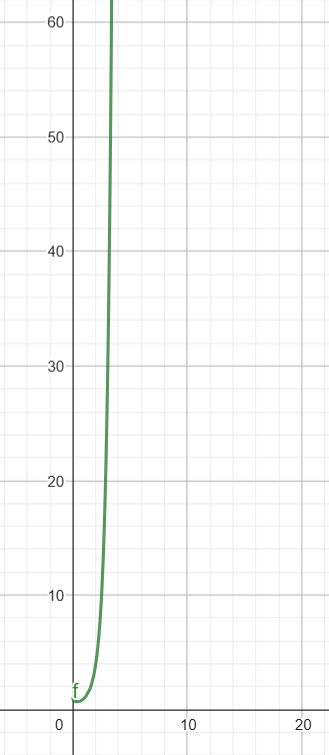
\includegraphics[height=12cm]{GraficoKelevK.png}
\caption{Gráfico da função $k^k$}
\label{fig:kelevk}
\end{figure}

O propósito do algoritmo então é garantir que o tempo possa ser diminuído de acordo com $k$, sem que seja necessário executar para todo $n-k$ restante.

\subsection{Explicação}
O algoritmo é dividido em duas funções principais, a \texttt{main} e a \texttt{defensiveAlliance}. A \texttt{main} recebe como entrada um Grafo $G$ e o tamanho da aliança desejada, um inteiro positivo $k$. De forma intuitiva, a abordagem do algoritmo é partir de um vértice do grafo por vez e olhar sua vizinhança numa tentativa de expandi-lo até formar uma aliança defensiva de tamanho $k$, ou todos os vértices terem servido de raiz da expansão.

\lstset{ 
  deletekeywords={do}  
}

\begin{lstlisting}[escapeinside={(*}{*)}]
Main(G,k)
	Para cada vértice v de G:
		v.c_w <- (*$\ceil{\frac{d(v)}{2}}$*).
	Para cada vértice v de G:
		inicia uma aliança S <- {v}.
		aliança_encontrada <- DefensiveAlliance(S).
		Se aliança_encontrada:
			retorne aliança_encontrada.
		retira v de S
		soma 1 ao c_w de v.
			
	retorne "Sem aliança";
\end{lstlisting}

O papel da função \texttt{main} é garantir que todos os vértices foram usados como raiz da expansão. Para isso, primeiro é definido o \texttt{c\_w}, que serve para verificar se o vértice está protegido dentro da aliança \texttt{S}. De início, ela é definida com o número de vizinhos necessários dentro de $S$ para que ele esteja defendido, e então será aumentada ou diminuida conforme se adiciona ou remove seus vizinhos a $S$.

Isso também faz parte da condição de sucesso da busca, ou seja, quando todos os vértices de \texttt{S} estiverem protegidos (\texttt{c\_w <= 0}) então uma aliança defensiva foi formada.

A seguir, a \texttt{main} chama a função \texttt{defensiveAlliance} para verificar se \texttt{S} é, ou pode ser expandida até, uma aliança defensiva de tamanho \texttt{k}.

\begin{lstlisting}[escapeinside={(*}{*)}]
DefensiveAlliance(G, S, k)
	inicia v <- vértice de maior c_w em S.
	Se v.c_w <= 0 e tamanho de S == k:
		devolve S.
		
	Se v.c_w <= k - tamanho de S: 
		inicia t <- 1 + metade dos vizinhos de w.
		inicia o conjunto W <- t vizinhos de w que não pertencem a S.
		Para cada vértice w em W:
			S <- S + w.
			Para cada vizinho x de w em S:
				subtrai 1 do c_w de x e de w.
			aliança_encontrada <- DefensiveAlliance(G, S, k)
			Se aliança_encontrada:
				Devolve aliança_encontrada.
			Para cada vizinho x de w em S:
				soma 1 ao c_w de x e de w.
			Retira w de S.
			
	Retorne NULL;
\end{lstlisting}

No início de \texttt{defensiveAlliance} o algoritmo escolhe o vértice de maior \texttt{c\_w} em \texttt{S},  que seria o vértice mais vulnerável da aliança. Esse vértice serve para tanto verificar se \texttt{S} se tornou uma aliança quanto como ponto de expansão a fim de incluir novos vértices.

A seguir, o algoritmo verifica se há espaço em \texttt{S} para os \texttt{c\_w} vizinhos necessários serem adicionados, ou seja, para que \texttt{w} seja defendido dentro da restrição do tamanho máximo \texttt{k}. Essa verificação funciona de modo semelhante a uma heurística de busca, poupando tempo ao evitar vértices que não podem ser defendidos posteriormente.

\subsection{Lema 14}
Uma parte importante do funcionamento do algoritmo é o lema 14 de \cite{Enciso2009}. Assuma que $S \subseteq V$ é estendível para uma aliança defensiva S', onde $|S| <|S'| = k$ então, para qualquer vértice desprotegido $w \in S$, $|S' \cap (N[w] - S|) \ge c_w$.\\
Em outras palavras se $S$ é estendível e $w$ é um vértice desprotegido de $S$ então $c_w$ é o número de vizinhos de $w$ fora de $S$ que é necessário para proteger $w$ em $S$.

Esse lema é o que podemos considerar como o núcleo do algoritmo, pois ele nos garante também que para qualquer subconjunto $W \subseteq N[w] - S$ com $t = \lfloor \frac{d_w}{2} \rfloor + 1$  vértices contém ao menos um vértice $w_i$ para o qual $S \cup {w_i}$ é estendível se e somente se S é estendível.

\subsection{Evitando repetir conjuntos}
Observando o comportamento do algoritmo no visualizador web foi possível notar que um comportamento pouco eficiente: o critério de expansão de $S$ (destacado a seguir) abre margem pra repetir várias vezes a mesma combinação de vértices, levando, principalmente em grafos de grande quantidade de vértices, a muito esforço improdutivo.

\begin{lstlisting}
DefensiveAlliance(G, S, k)
	inicia v <- vértice de maior c_w em S.
\end{lstlisting}

Pensando nisso a equipe elaborou uma solução que armazena todas as combinações já analisadas anteriormente e impede de que novas iterações com elas sejam geradas, cortando toda a sub-árvore subsequente. Isso é feito com a criação de um dicionário e a marcação única de cada combinação:

\begin{lstlisting}
inicia combinacoes <- dicionário vazio
\end{lstlisting}

\begin{lstlisting}
DefensiveAlliance(G, S, k)
[...]
	Para cada vértice w em W:
		S <- S + w.
		
		comb_id <- identificadores de S de forma ordenada.
		Se existe combinacoes[comb_id]:
			Retira w de S.
			pula para o próximo vértice.
		Caso contrário:	
			cria combinacoes[comb_id].

		Para cada vizinho x de w em S:
			subtrai 1 do c_w de x e de w.
		aliança_encontrada <- DefensiveAlliance(G, S, k)
[...]
\end{lstlisting}

Caso não exista uma entrada da combinação no dicionário, cria-se uma e a instância corrente de \texttt{S} é analisada. Caso contrário, a instância é ignorada, podando todas as sub-árvores subsequentes. A complexidade de tempo é se resume a ordenação de, no máximo, $k-1$ elementos, e ao acesso e escrita no dicionário. Ambos são ofuscados pela complexidade geral.

Por outro lado, há um custo sério em termos de espaço. No pior caso, de não haver aliança e o algoritmo analisar todos os vértices e $k=n$, a combinação ocupa espaço $O(2^n)$, que corresponde a guardar todas as combinações de $n$ vértices, variando de tamanho $1$ até $n$. Isso pode ser mitigado ao limitar o tamanho das combinações armazenadas para a região crítica que vai ser repetida mais vezes. A análise desta região está na seção sobre Resultados e discussão.

Quanto ao desempenho, esta técnica permite ao algoritmo poupar muito tempo ao "amortizar" o custo $k^k$ ao longo de várias iterações, pois, como nenhuma combinação é repetida, quanto mais exploradas são as combinações dos vértices, menos combinações existem para serem analisadas.

\subsection{Priorização dos vértices expostos}
\begin{lstlisting}
DefensiveAlliance(G, S, k)
	inicia v <- vértice de maior c_w em S.
\end{lstlisting}

Ao iniciarmos $DefensiveAlliance(G,S,k)$ atribuindo $v$ o vértice em $W$ com maior $c_w$ nós garantimos que a maior prioridade em cada chamada recursiva da função é proteger o vértice mais "exposto".

Assim obtemos também um critério de parada consistente, ou seja, quando o vértice com maior $c_w$ ter $c_w \le 0$ e $|S| = k$, teremos duas informações fundamentais sobre o contexto da execução:\\
1 - Se $c_w \le 0$, então todos os vértices em $S$ estão protegidos.\\
2 - Se $|S|=k$, encontramos a aliança defensiva procurada.

\chapter{Metodologia}
O projeto é composto por duas partes principais: algoritmos de busca implementados em Python e um visualizador web criado para exibir os passos deste algoritmo. As partes funcionam de forma independente, sendo conectadas apenas pelo formato de entrada e saída dos programas.

\section{Algoritmo em Python}
A implementação do algoritmo proposto por \cite{Enciso2009} foi feita em Python e consta completa no Apêndice 1.

Nesta implementação foi utilizada a estrutura de dados da biblioteca \textit{Networkx} para manipulação dos grafos, e, no mais, estruturada de forma semelhante ao algoritmo teórico, com a exceção do uso de uma estrutura de pilha para substituir a chamada recursiva.

Além do resultado final, o programa possibilita o retorno da aliança em formato JSON, com as características utilizadas no visualizador web. Essas características permitem a visualização passo a passo dos nós expandidos pelo algoritmo, e consistem do conjunto $W$ a cada iteração da função \texttt{DefensiveAlliance}.

Há também \textit{flags} para mostrar a quantidade de nós expandidos, para gerar um grafo aleatório segundo uma densidade especificada, e para alterar o comportamento da busca, como retornar a primeira aliança encontrada independente do tamanho.

\section{Visualizador web}
O projeto web foi desenvolvido com Typescript e React, e sua proposta é fornecer uma visualização passo-a-passo do algoritmo e do grafo de entrada. Assim como o algoritmo de busca, o visualizador pode ser encontrado no repositório que se encontra nas referências.

Para montar a visualização é necessário que seja fornecido como entrada um grafo disposto em formato JSON, contando com dois conjuntos extras de dados que são a aliança encontrada, caso exista, e um vetor de \textit{steps}, que contém o conjunto $W$ no dado \textit{passo} da iteração.

Munido destas informações, o visualizador organiza os dados internamente para melhorar o desempenho e a decisão de cada caraterística visual do grafo e então personaliza uma \textit{view} HTML, dada pela biblioteca 3d-force-graph \cite{HassanShafique2004}, que cuida da renderização e simulação física do grafo.

Dentre as funcionalidades, vale destacar duas principais: a visualização do conjunto $S$ a cada etapa do algoritmo e o mapa de calor dos nós explorados. O mapa de calor é a coloração dos vértices do grafo seguindo a regra de que, quanto mais visitado um vértice durante a execução do algoritmo, mais quente é a cor usada; os nós mais quentes tem cores próximas do vermelho, e os mais frios, mais próximas do azul.

\subsection{Visualização por passos}
Ao carregar um grafo com o conjunto de passos, é possível navegar por cada um deles. Em um certo passo, os vértices e arestas da fronteira de $S$ são desenhados com uma cor cinza escura, os além da fronteira tem cor cinza claro, e os vértices dentro de $S$ ficam coloridos com a cor

\begin{itemize}
  \item azul, se estiverem desprotegidos;
  \item ou verde, se estiverem devidamente protegidos.
\end{itemize}

Ao finalizar o algoritmo e desenhar a aliança, ela é colorida de verde escuro.

As figuras a seguir são de uma busca por uma aliança de tamanho $k = 15$ em um grafo de $v=50$ vértices e $e=40$ arestas. O algoritmo começa com $S$ contendo o vértice colorido de azul.

\begin{figure}[!htb]
\centering
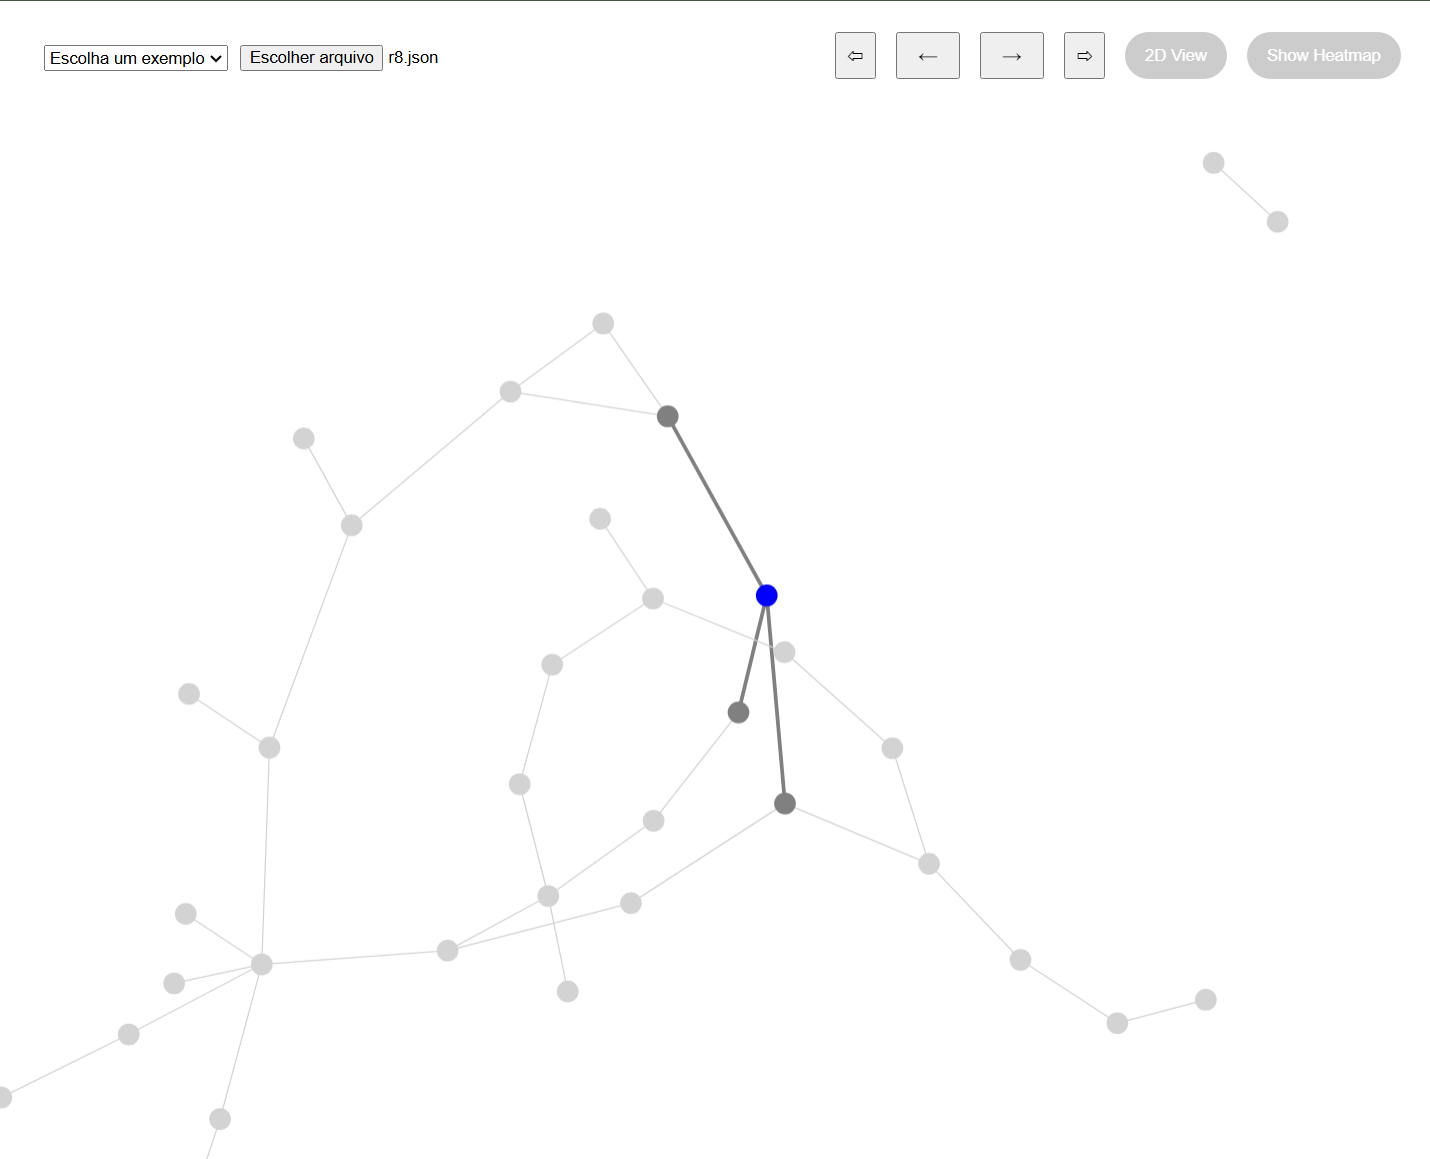
\includegraphics[width=12cm]{GrafoSteps1.png}
\caption{Passo 1 do algoritmo}
\label{fig:grafo-steps-1}
\end{figure}

\begin{figure}[!htb]
\centering
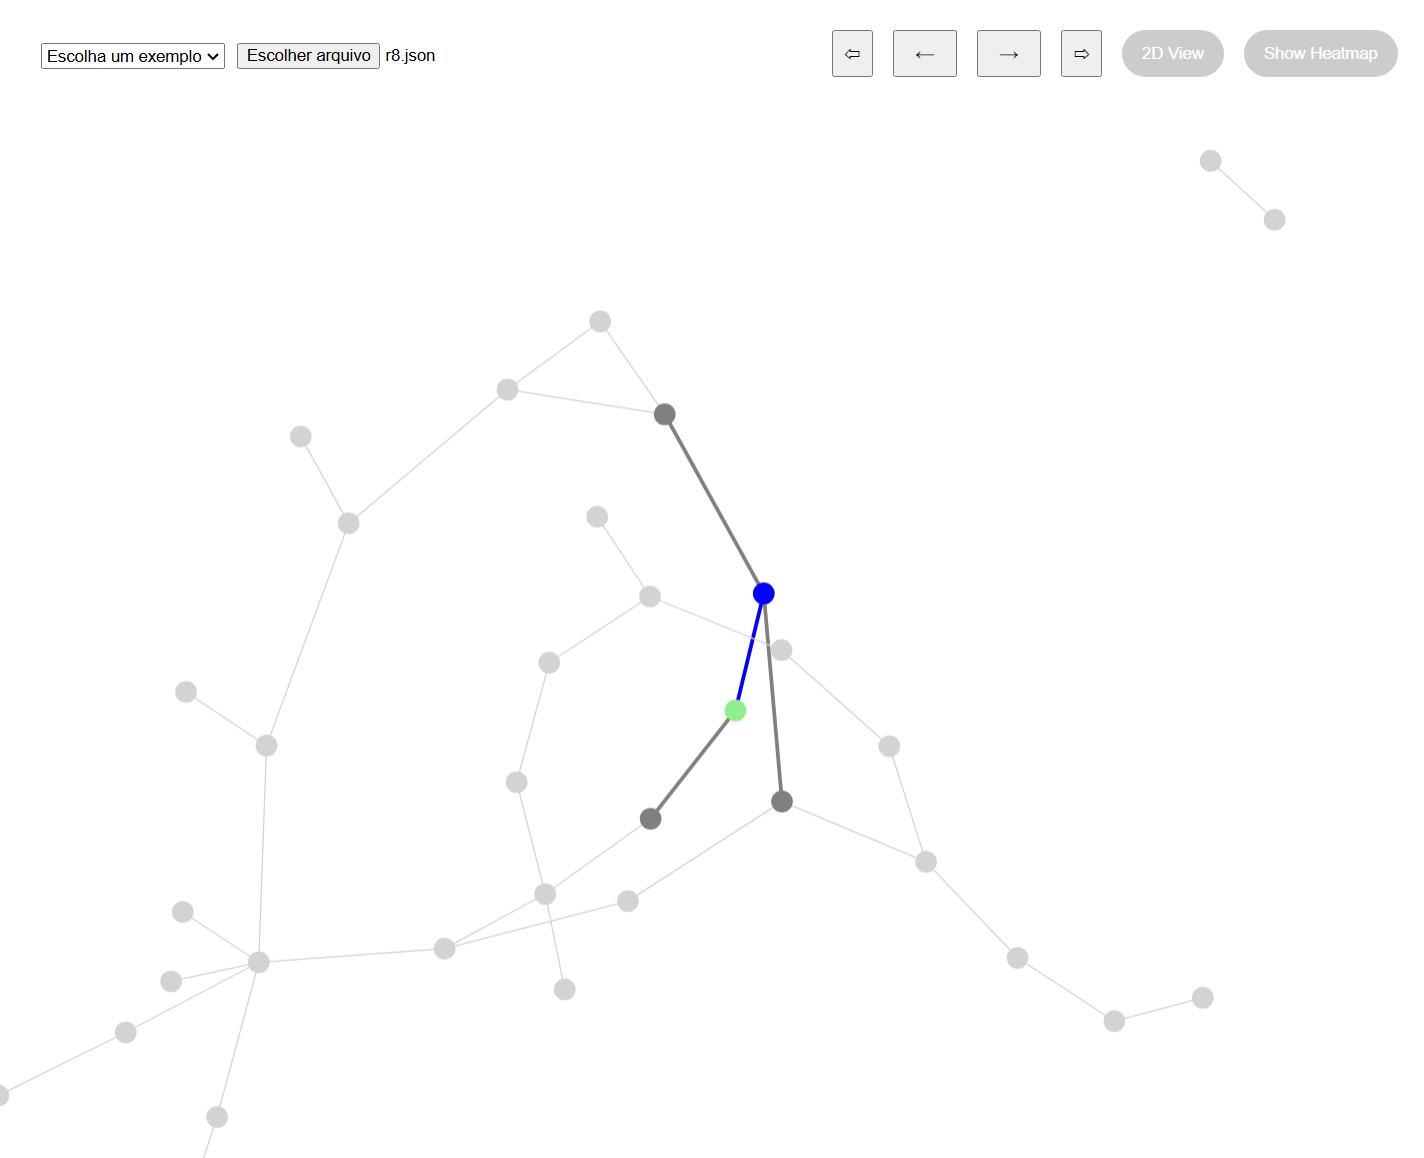
\includegraphics[width=12cm]{GrafoSteps2.png}
\caption{Passo 2 do algoritmo}
\label{fig:grafo-steps-2}
\end{figure}

\begin{figure}[!htb]
\centering
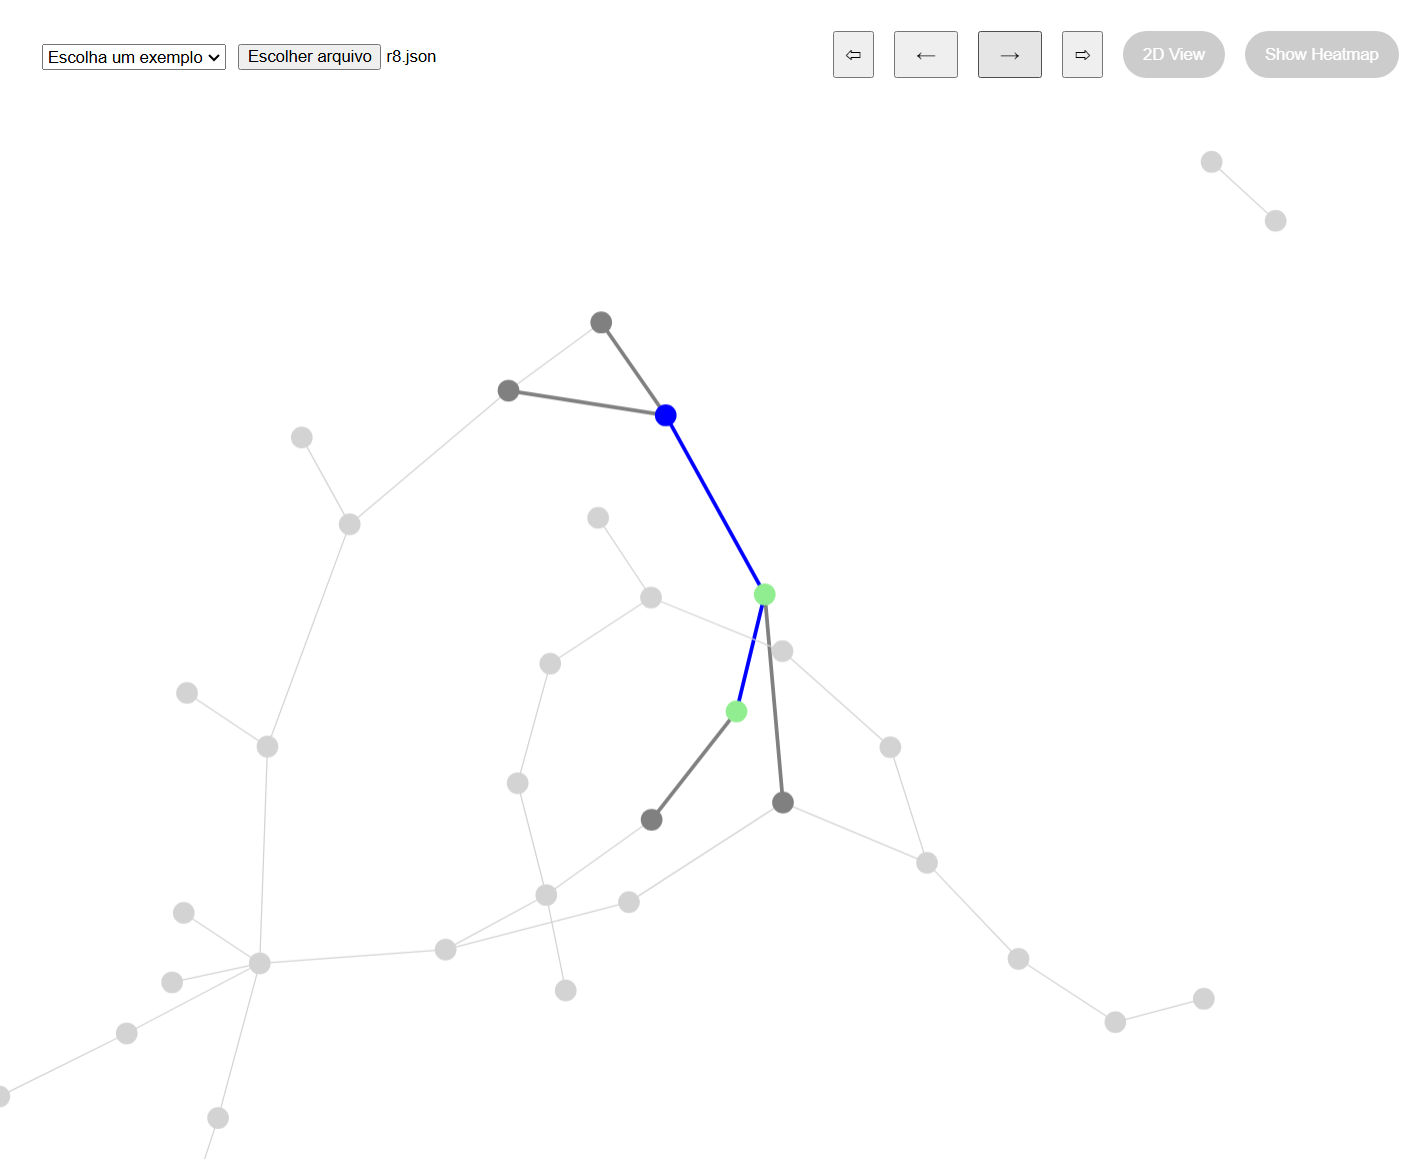
\includegraphics[width=12cm]{GrafoSteps3.png}
\caption{Passo 3 do algoritmo}
\label{fig:grafo-steps-3}
\end{figure}

\begin{figure}[!htb]
\centering
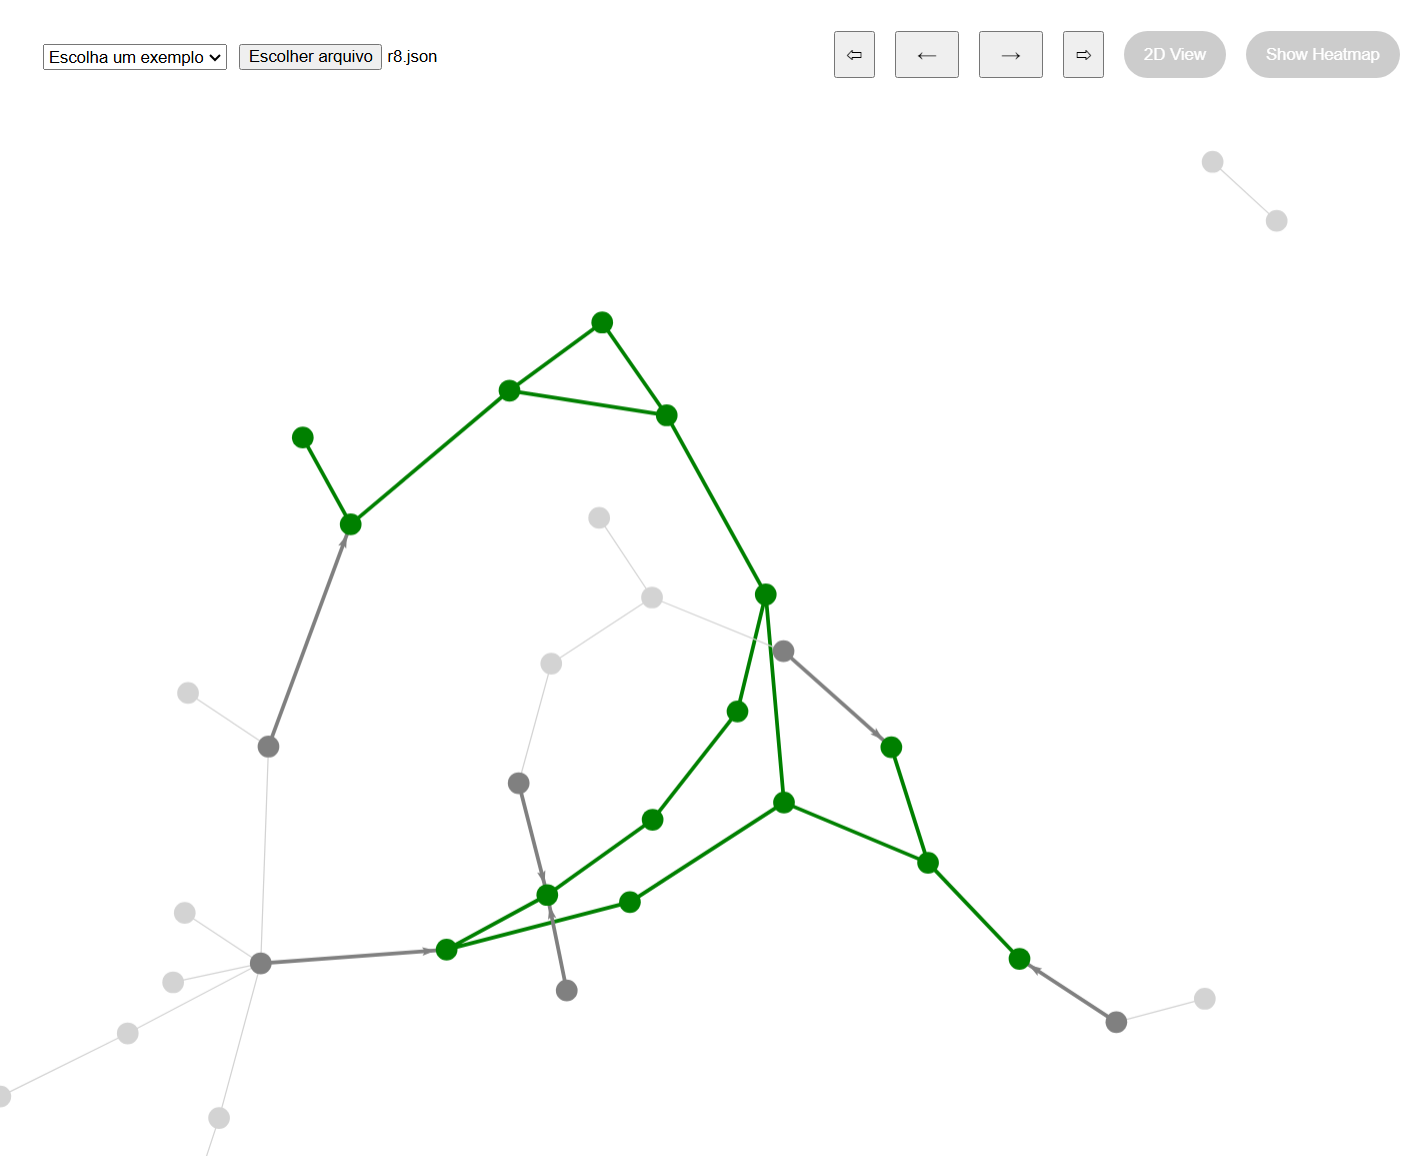
\includegraphics[width=12cm]{GrafoStepsN.png}
\caption{Passo final do algoritmo}
\label{fig:grafo-steps-n}
\end{figure}

\subsection{Mapa de calor}
É possível também ativar a visualização do mapa de calor, que colore os vértices de acordo com a quantidade de vezes que ele foi explorado pelo algoritmo.

\begin{figure}[!htb]
\centering
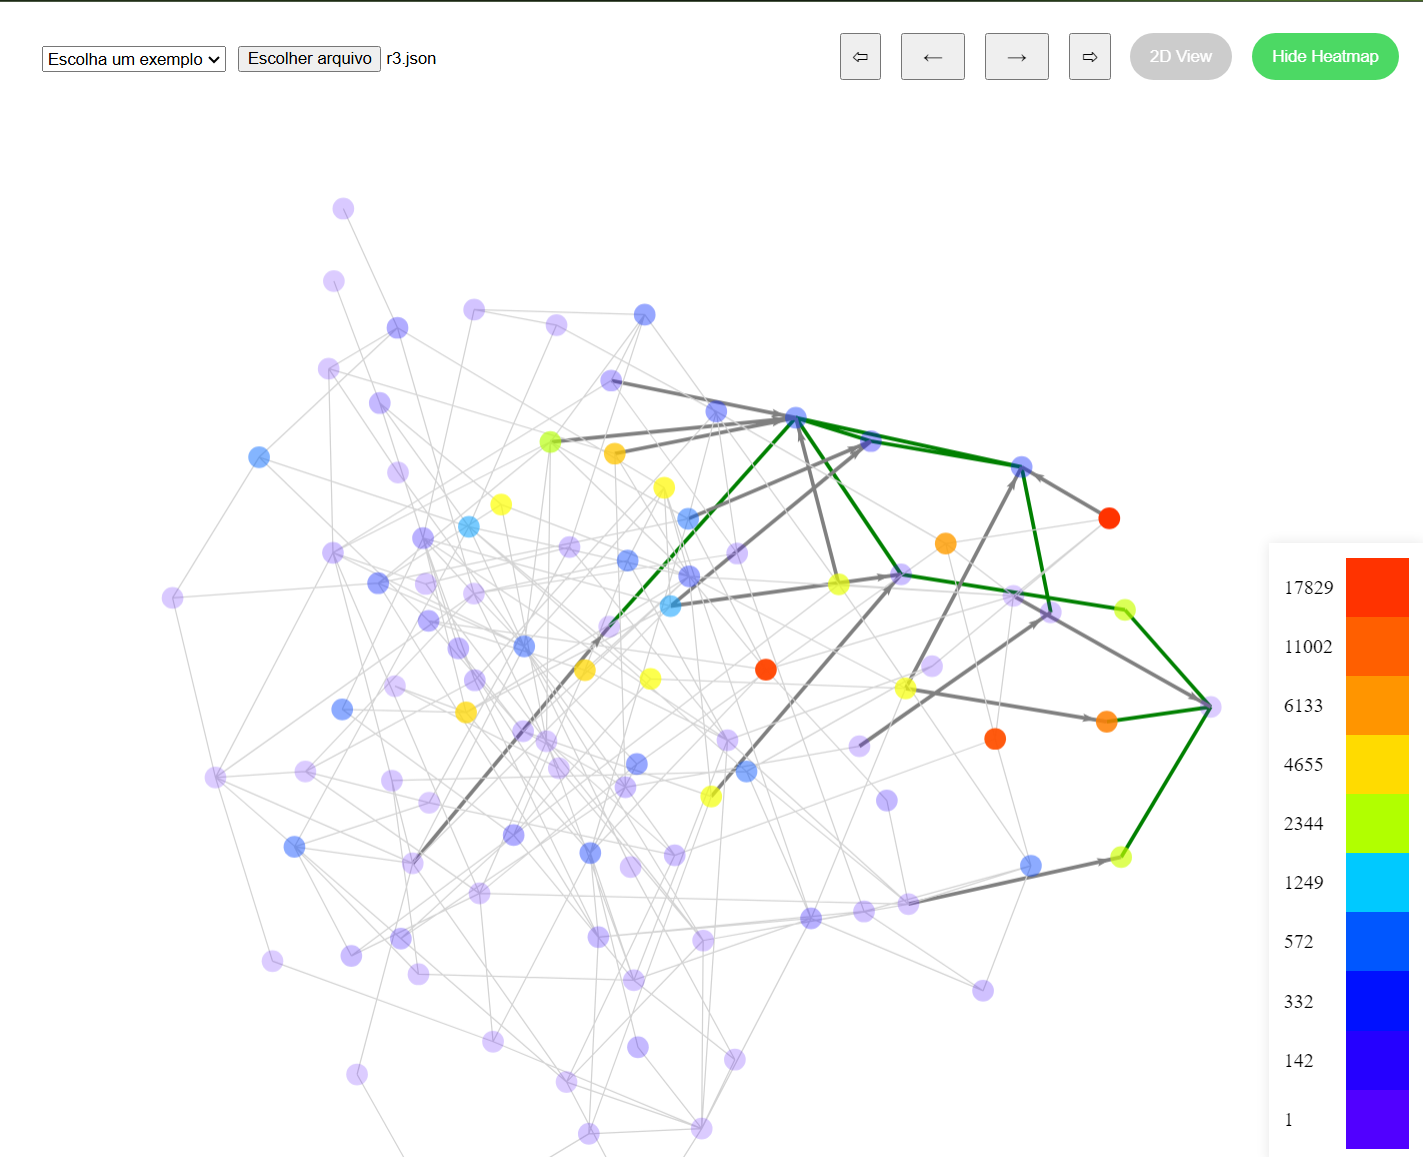
\includegraphics[width=12cm]{GrafoHeatmap.png}
\caption{Mapa de calor do grafo}
\label{fig:grafo-heatmap}
\end{figure}

Para ajudar na visualização, as cores mais frias também tem opacidade mais baixa.

Essa ferramenta em particular incentivou questionamentos interessantes a respeito da eficiência do algoritmo, como "como evitar a alta taxa de repetição de um grupo de vértices".

\chapter{Resultados e discussão}
O algoritmo originalmente estudado e a versão com as melhorias propostas foram analisadas e submetidas a um conjunto de testes para melhor ilustrar o impacto e eficiência de cada uma. Visto que o problema continua sendo NP-completo, há pouco a ser feito para valores realmente grandes, mas foi possível sim observar uma ampliação dos valores considerados "razoáveis" pelo algoritmo FPT.

Para testar o algoritmo utilizamos a função da biblioteca \texttt{networkx nx.erdos\_renyi\_graph(v,e,seed)} onde \texttt{v} é o número de vértices \texttt{e} é a probabilidade de 2 vértices formarem uma aresta, e \texttt{seed} é uma semente para geração do Grafo.

Para os testes a seguir foram fixados os seguintes seguintes parâmetros \texttt{v=30} \texttt{e=0.333} e \texttt{seed=100} e executamos para \texttt{k} variando entre \texttt{1} e \texttt{29}.

\begin{figure}[!htb]
\centering
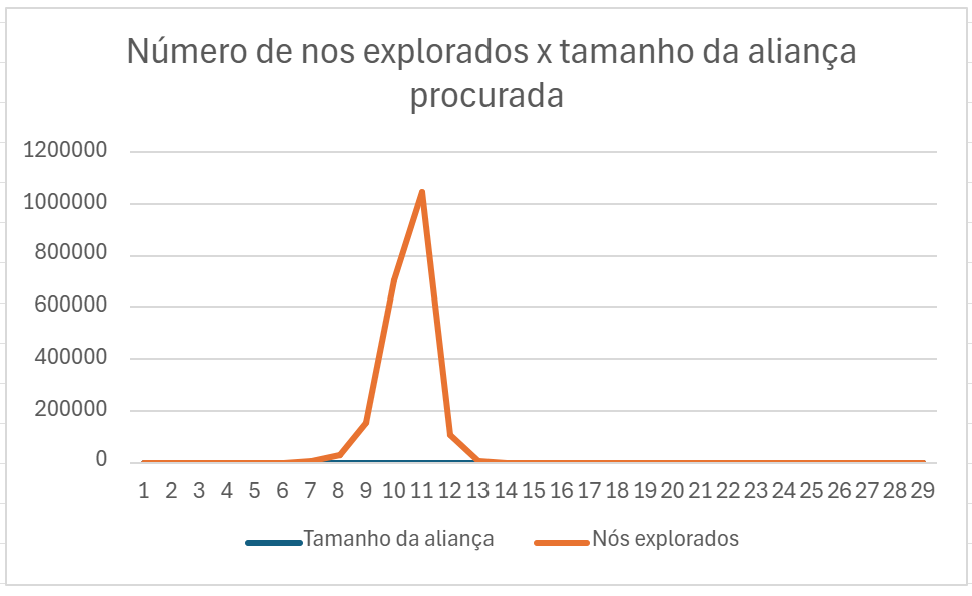
\includegraphics[width=12cm]{Execução sem repetição de conjuntos.png}
\caption{Execução do algoritmo \textbf{evitando} a repetição de conjuntos}
\label{fig:execucao-sem-repeticao}
\end{figure}

Na execução do algoritmo sem repetição de conjuntos é possível notar que o número máximo de nós explorados foi de aproximadamente 1 milhão de nós.

\begin{figure}[!htb]
\centering
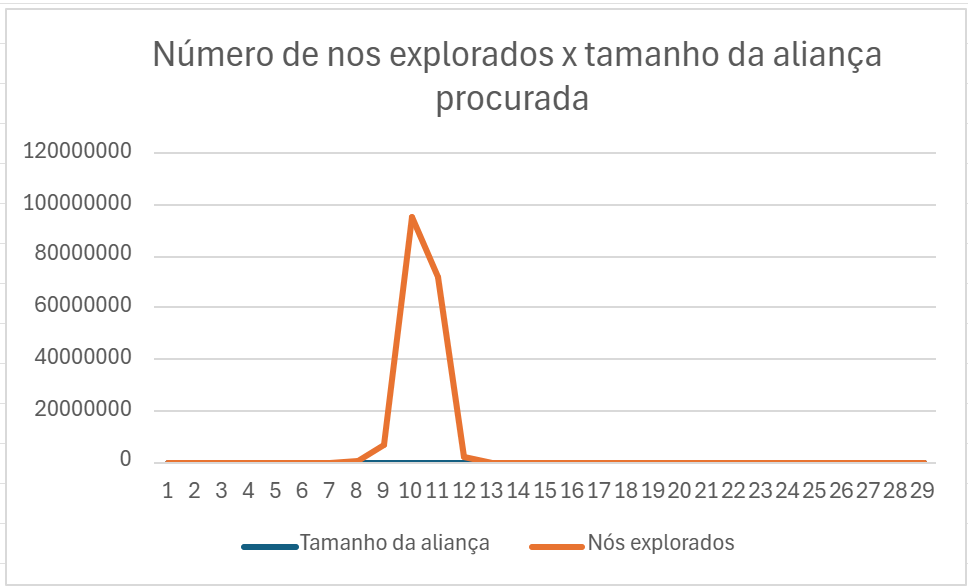
\includegraphics[width=12cm]{Execução com repetição de conjuntos.png}
\caption{Execução do algoritmo \textbf{permitindo} a repetição de conjuntos}
\label{fig:execucao-com-repeticao}
\end{figure}

Por sua vez, na execução que permite a repetição de conjuntos o número de nós explorados nesse caso saltou de 1 milhão para 100 milhões.

Salvar os conjuntos resulta em uma melhora significativa na redução do número de nós a serem explorados, porém nós traz um novo problema pois o espaço necessário para armazenar todos esses conjuntos no pior caso é $\sum_{i=0}^{k} \binom{n}{i}<2^n$, ou seja, acabamos trocando um tempo exponencial, por espaço exponencial.

Foi observado um padrão interessante na eficiência com relação ao grau médio dos vértices do grafo $d(G)$ e $k$; o número de nós explorados atinge um ápice para valores de $k$ próximos de $d(G)$ criando uma "zona difícil", e suaviza a medida que a diferença aumenta.

Para valores de $d(G)$ muito maiores que $k$ isso acontece porque o algoritmo pode descartar muitas combinações através do critério \texttt{Se v.c\_w <= k - tamanho de S:}. Essa linha garante que o próximo nó a ser expandido ao menos tem as condições de ser protegido dado o tamanho atual de $S$.

Por outro lado, valores de $k$ muito menores do que $d(G)$, foi observado uma probabilidade maior de haver uma aliança defensiva. A modificação de ordenação dos vértices de \texttt{W} com base em quantos vizinhos ele possui em $S$ e $\lfloor d(v)/2 \rfloor$, em especial, mostrou acelerar muito o processo de determinação da aliança, quando existente. Isso se deve as escolhas priorizarem a defesa dos vértices já em $S$, em prol de adições aleatórias.

Por fim, a modificação de "Evitar repetir conjuntos" mostrou-se acelerar o processo tanto no melhor caso quanto no pior, pois garante que somente novas combinações são testadas.

\chapter{Conclusão}
O estudo como um todo foi bastante produtivo dentro do tema, e possibilitou compreensão significativa do que são e como encontrar alianças defensivas. O visualizador web, como ferramenta didática, foi bastante aproveitado para a compreensão e elaboração das melhorias propostas ao algoritmo.

Também foi produtivo experimentar na prática a complexidade de um problema NP-completo e uma das ferramentas usadas para contornar esse degrau gigantesco na complexidade.

Dentre os diversos temas que podem ser abordados em discussões futuras, destacamos a implementação e análise do algoritmo proposto por \cite{Enciso2009} para encontrar Conjuntos Seguros (\textit{Secure Sets}), que segue uma abordagem FPT semelhante ao de alianças defensivas, e pode ser adaptado para o visualizador web para gerar resultados valiosos.

Outro ponto de possível expansão é o de pré-análise de grafos para a determinação de potencial de uma aliança de tamanho $k$, partindo da análise feita sobre o grau médio e a "zona difícil".
		% experimentação e validação
%\chapter{Fundamentação teórica}
A fim de seguir de forma devida com a análise do problema e do algoritmo, algumas definições teóricas são requeridas:

\section{Conceitos}

\subsection{Grafo}
Um grafo $G = (V(G), E(G))$ é um par ordenado que consiste de um conjunto de vértices $V(G)$ e um conjunto de arestas $E(G)$.

\subsection{Vértice}
Um vértice $v \in V(G)$ é um elemento básico de um grafo, representando um ponto ou nó na estrutura. O conjunto $V(G)$ é finito e contém todos os vértices do grafo.

\subsection{Aresta}
Uma aresta $e \in E(G)$ é um conjunto de dois vértices de $V(G)$. Em um grafo não direcionado, a aresta $\{u, v\}$ conecta os vértices $u$ e $v$, sem direção. Em grafos direcionados, uma aresta $(u, v)$ conecta $u$ a $v$ com uma orientação de $u$ para $v$.

\subsection{Incidência}
As extremidades de uma aresta são ditas incidentes com a aresta \cite{Bondy2008}, e vice-versa, ou seja, uma aresta $e$ é dita incidente a um vértice $v$ se está aresta se conecta a $v$ em um de seus extremos.

\subsection{Adjacência}
Dois vértices que são incidentes a uma mesma aresta são adjacentes \cite{Bondy2008}, assim como duas arestas que são incidentes a um mesmo vértice, ou seja, um par de vértices distintos $u$ e $v$ são adjacentes se possuem uma aresta que os conectam, da mesma forma que duas arestas distintas $e1$ e $e2$ são adjacentes se são incidentes a um vértice em comum.

\subsection{Vizinhança de um Vértice}
Dois vértices que são incidentes a uma aresta comum, ou seja, dois vértices adjacentes distintos são ditos vizinhos \cite{Bondy2008}. A vizinhança de um vértice $v \in V(G)$, denotada por $N(v)$, é o conjunto de todos os vértices adjacentes a $v$, ou seja, $N(v) = \{ u \in V(G) \mid \{u, v\} \in E(G) \}$ em grafos não direcionados.

\subsection{Grau de um Vértice}
O grau de um vértice $v$ em um grafo não direcionado $G$ é dado por $d(v) = |N(v)|$, ou seja, o número de arestas incidentes a $v$. Neste estudo consideramos apenas grafos não direcionados, portanto o grau de $v$ corresponde ao número de arestas total ligadas a ele.

\subsection{Subgrafo}
Um \textbf{subgrafo} de um grafo $G$ é um grafo $F$ cujos conjuntos de vértices e arestas são subconjuntos dos vértices e arestas de $G$. Formalmente, $F$ é um subgrafo de $G$ se $V(F) \subseteq V(G)$ e $E(F) \subseteq E(G)$, e a função que relaciona vértices e arestas em $F$ é a mesma que em $G$, mas restrita ao conjunto de arestas de $F$. Subgrafos podem ser formados a partir das operações de remoção de vértices e remoção de arestas.\\
Diz-se que $G$ contém $F$ ou que $F$ está contido em $G$, representado como $G \supseteq F$ ou $F \subseteq G$.

\subsection{Conectividade}
Um grafo é \textbf{conexo} se, para toda partição de seu conjunto de vértices em dois conjuntos não vazios $X$ e $Y$, existe uma aresta com uma extremidade em $X$ e a outra extremidade em $Y$, caso contrário, o grafo é desconexo. Em outras palavras, um grafo é desconexo se seu conjunto de vértices pode ser particionado em dois subconjuntos não vazios $X$ e $Y$ de modo que nenhuma aresta tenha uma extremidade em $X$ e outra em $Y$.

\subsection{Aliança Defensiva}
Um subconjunto $S \subseteq V$ é uma aliança defensiva se, para cada vértice $v \in S$, a condição a seguir é satisfeita:   $|N(v) \cap S| \geq |N(v) \setminus S|$.\\
Ou seja, para cada vértice $v$ na aliança $S$, o número de vértices adjacentes a $v$ dentro de $S$ deve ser pelo menos igual ao número de vértices adjacentes a $v$ fora de $S$.\\
Isso indica que os vértices $v$ na aliança devem possuir pelo menos tantos vértices dentro da aliança quanto fora dela.\\
Embora, formalmente, uma aliança não precise ser conexa, note que cada componente conexa de uma aliança é uma aliança por si só. Para fins deste trabalho, toda aliança encontrada deve ser \textbf{conexa}.

\section{Complexidade Computacional}
A complexidade computacional estuda a quantidade de recursos necessários para a execução de algoritmos, especialmente em termos de tempo e espaço. Em ciência da computação, a complexidade computacional é frequentemente representada usando a notação \textit{Big O}, $O(f(n))$, que descreve o crescimento da complexidade como uma função $f(n)$, onde $n$ normalmente é o tamanho da entrada, ou algum outro parâmetro relevante. Alguns exemplos de classificação de complexidade são:

\begin{itemize}
  \item $O(1)$: Constante, o tempo de execução não depende do tamanho da entrada.
  \item $O(n)$: Linear, o tempo de execução cresce proporcionalmente ao tamanho da entrada.
  \item $O(n^k)$: Polinomial, o tempo de execução cresce proporcionalmente com relação a potência $k$ constante do tamanho da entrada. Um exemplo de polinômio muito comum são os quadrados $O(n^2)$.
  \item $O(k^n)$: Exponencial, o tempo de execução cresce de forma exponencial com relação ao tamanho da entrada. No geral, é inviável para grandes entradas.
  \item $O(n!)$ Fatorial, em problemas fatoriais o tempo de execução cresce ainda mais acelerado com relação ao tamanho da entrada do que problemas exponenciais.
\end{itemize}

\subsection{Classes de Complexidade:}
Os problemas de decisão, como os envolvendo alianças, podem ser classificados em certas classes de complexidade que separam o quão viáveis é encontrar ou verificar suas soluções para entradas de larga escala. Estas classes não:

\begin{itemize}
  \item $P$ (Polinomial): Representa a classe de problemas que podem ser resolvidos em tempo polinomial, ou seja, em $O(n^k)$ para algum inteiro $k$. Em ciência da computação, problemas em $P$ são considerados tratáveis.
  \item $NP$ (Tempo polinomial não determinístico): Representa a classe de problemas para os quais, apesar de não sabermos como encontrar solução em tempo polinomial de maneira determinística, dada uma solução, ela pode ser verificada em tempo polinomial por um algoritmo determinístico. Não sabemos se todo problema em $NP$ pode ser resolvido em tempo polinomial, isto é, se $P = NP$, e esse é um dos 7 problemas do milênio que ainda estão em aberto.
  \item $NP$-completo: Representa um subconjunto de problemas em $NP$ que são, intuitivamente, tão difíceis quanto qualquer outro problema em $NP$. Para um problema ser dessa classe, são necessárias duas características:
  \begin{enumerate}
    \item Estar em $NP$, ou seja, dada uma solução, ela deve ser verificável em tempo polinomial.
    \item Ser $NP$-difícil, todo problema em $NP$ pode ser redutível a ele em tempo polinomial.\\
Em outras palavras, caso um problema de classe $NP$-completo seja resolvido em tempo polinomial, todos os outros problemas em $NP$ poderão ser resolvidos em tempo polinomial.
  \end{enumerate}
\end{itemize}

\section{O algoritmo}
Como encontrar uma aliança defensiva em um grafo é um problema NP-completo, o algoritmo FPT \cite{Enciso2009} tem como objetivo buscar por uma aliança conexa arbitrária de tamanho máximo $k$, a fim de tornar o problema tratável. Porém, neste trabalho o tamanho da aliança buscada será \textit{exatamente} $k$, pois acreditamos que o tamanho da aliança seja importante. Antes de entrar na explicação minuciosa do algoritmo, é importante explicar o que é um algoritmo FPT.

\subsection{Complexidade}
FPT (\textit{Fixed-Parameter Tractable}) é uma classe de complexidade que trata de problemas parametrizáveis (como os de complexidade exponencial) ao isolar e fixar um parâmetro específico do problema, chamado $k$, e então expressando a complexidade na forma $f(k)*p(n).$ Desta forma, $f(k)$ é a parte da complexidade que depende exclusivamente de $k$ e pode ser \textit{superpolinomial}, enquanto $p(n)$ é uma função polinomial de $n$. Sendo assim, fixar $k$ em valores pequenos nos permite abordar o algoritmo de forma mais tratável, custando muito menos tempo, a depender do tamanho de $k$.

O algoritmo usado neste estudo foi proposto por \cite{Enciso2009}, e tem complexidade $O(k^kn)$, e é uma melhora significativa de seu predecessor, que tinha complexidade $O((2k-1)^kk^2n)$. Esse é um avanço substancial, mas ainda é interessante demonstrar como problemas, mesmo parametrizados, crescem rapidamente:

\begin{table}[h]
\begin{center}
\begin{tabular}{|c|c|c|c|c|c|c|c|}
\hline
$k$ & $k^k$\\
\hline
2 & 4 \\
\hline
3 & 27 \\
\hline
4 & 256 \\
\hline
5 & 3.125 \\
\hline
6 & 46.656 \\
\hline
7 & 823.543 \\
\hline
9 & 387.420.489 \\
\hline
10 & 10.000.000.000 \\
\hline
\end{tabular}
\end{center}
\end{table}

\begin{figure}[!htb]
\centering
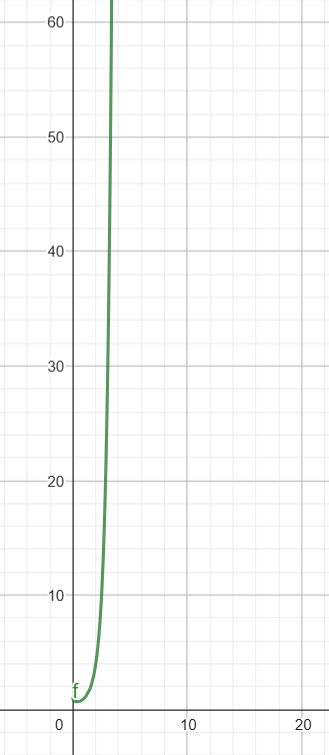
\includegraphics[height=12cm]{GraficoKelevK.png}
\caption{Gráfico da função $k^k$}
\label{fig:kelevk}
\end{figure}

O propósito do algoritmo então é garantir que o tempo possa ser diminuído de acordo com $k$, sem que seja necessário executar para todo $n-k$ restante.

\subsection{Explicação}
O algoritmo é dividido em duas funções principais, a \texttt{main} e a \texttt{defensiveAlliance}. A \texttt{main} recebe como entrada um Grafo $G$ e o tamanho da aliança desejada, um inteiro positivo $k$. De forma intuitiva, a abordagem do algoritmo é partir de um vértice do grafo por vez e olhar sua vizinhança numa tentativa de expandi-lo até formar uma aliança defensiva de tamanho $k$, ou todos os vértices terem servido de raiz da expansão.

\lstset{ 
  deletekeywords={do}  
}

\begin{lstlisting}[escapeinside={(*}{*)}]
Main(G,k)
	Para cada vértice v de G:
		v.c_w <- (*$\ceil{\frac{d(v)}{2}}$*).
	Para cada vértice v de G:
		inicia uma aliança S <- {v}.
		aliança_encontrada <- DefensiveAlliance(S).
		Se aliança_encontrada:
			retorne aliança_encontrada.
		retira v de S
		soma 1 ao c_w de v.
			
	retorne "Sem aliança";
\end{lstlisting}

O papel da função \texttt{main} é garantir que todos os vértices foram usados como raiz da expansão. Para isso, primeiro é definido o \texttt{c\_w}, que serve para verificar se o vértice está protegido dentro da aliança \texttt{S}. De início, ela é definida com o número de vizinhos necessários dentro de $S$ para que ele esteja defendido, e então será aumentada ou diminuida conforme se adiciona ou remove seus vizinhos a $S$.

Isso também faz parte da condição de sucesso da busca, ou seja, quando todos os vértices de \texttt{S} estiverem protegidos (\texttt{c\_w <= 0}) então uma aliança defensiva foi formada.

A seguir, a \texttt{main} chama a função \texttt{defensiveAlliance} para verificar se \texttt{S} é, ou pode ser expandida até, uma aliança defensiva de tamanho \texttt{k}.

\begin{lstlisting}[escapeinside={(*}{*)}]
DefensiveAlliance(G, S, k)
	inicia v <- vértice de maior c_w em S.
	Se v.c_w <= 0 e tamanho de S == k:
		devolve S.
		
	Se v.c_w <= k - tamanho de S: 
		inicia t <- 1 + metade dos vizinhos de w.
		inicia o conjunto W <- t vizinhos de w que não pertencem a S.
		Para cada vértice w em W:
			S <- S + w.
			Para cada vizinho x de w em S:
				subtrai 1 do c_w de x e de w.
			aliança_encontrada <- DefensiveAlliance(G, S, k)
			Se aliança_encontrada:
				Devolve aliança_encontrada.
			Para cada vizinho x de w em S:
				soma 1 ao c_w de x e de w.
			Retira w de S.
			
	Retorne NULL;
\end{lstlisting}

No início de \texttt{defensiveAlliance} o algoritmo escolhe o vértice de maior \texttt{c\_w} em \texttt{S},  que seria o vértice mais vulnerável da aliança. Esse vértice serve para tanto verificar se \texttt{S} se tornou uma aliança quanto como ponto de expansão a fim de incluir novos vértices.

A seguir, o algoritmo verifica se há espaço em \texttt{S} para os \texttt{c\_w} vizinhos necessários serem adicionados, ou seja, para que \texttt{w} seja defendido dentro da restrição do tamanho máximo \texttt{k}. Essa verificação funciona de modo semelhante a uma heurística de busca, poupando tempo ao evitar vértices que não podem ser defendidos posteriormente.

\subsection{Lema 14}
Uma parte importante do funcionamento do algoritmo é o lema 14 de \cite{Enciso2009}. Assuma que $S \subseteq V$ é estendível para uma aliança defensiva S', onde $|S| <|S'| = k$ então, para qualquer vértice desprotegido $w \in S$, $|S' \cap (N[w] - S|) \ge c_w$.\\
Em outras palavras se $S$ é estendível e $w$ é um vértice desprotegido de $S$ então $c_w$ é o número de vizinhos de $w$ fora de $S$ que é necessário para proteger $w$ em $S$.

Esse lema é o que podemos considerar como o núcleo do algoritmo, pois ele nos garante também que para qualquer subconjunto $W \subseteq N[w] - S$ com $t = \lfloor \frac{d_w}{2} \rfloor + 1$  vértices contém ao menos um vértice $w_i$ para o qual $S \cup {w_i}$ é estendível se e somente se S é estendível.

\subsection{Evitando repetir conjuntos}
Observando o comportamento do algoritmo no visualizador web foi possível notar que um comportamento pouco eficiente: o critério de expansão de $S$ (destacado a seguir) abre margem pra repetir várias vezes a mesma combinação de vértices, levando, principalmente em grafos de grande quantidade de vértices, a muito esforço improdutivo.

\begin{lstlisting}
DefensiveAlliance(G, S, k)
	inicia v <- vértice de maior c_w em S.
\end{lstlisting}

Pensando nisso a equipe elaborou uma solução que armazena todas as combinações já analisadas anteriormente e impede de que novas iterações com elas sejam geradas, cortando toda a sub-árvore subsequente. Isso é feito com a criação de um dicionário e a marcação única de cada combinação:

\begin{lstlisting}
inicia combinacoes <- dicionário vazio
\end{lstlisting}

\begin{lstlisting}
DefensiveAlliance(G, S, k)
[...]
	Para cada vértice w em W:
		S <- S + w.
		
		comb_id <- identificadores de S de forma ordenada.
		Se existe combinacoes[comb_id]:
			Retira w de S.
			pula para o próximo vértice.
		Caso contrário:	
			cria combinacoes[comb_id].

		Para cada vizinho x de w em S:
			subtrai 1 do c_w de x e de w.
		aliança_encontrada <- DefensiveAlliance(G, S, k)
[...]
\end{lstlisting}

Caso não exista uma entrada da combinação no dicionário, cria-se uma e a instância corrente de \texttt{S} é analisada. Caso contrário, a instância é ignorada, podando todas as sub-árvores subsequentes. A complexidade de tempo é se resume a ordenação de, no máximo, $k-1$ elementos, e ao acesso e escrita no dicionário. Ambos são ofuscados pela complexidade geral.

Por outro lado, há um custo sério em termos de espaço. No pior caso, de não haver aliança e o algoritmo analisar todos os vértices e $k=n$, a combinação ocupa espaço $O(2^n)$, que corresponde a guardar todas as combinações de $n$ vértices, variando de tamanho $1$ até $n$. Isso pode ser mitigado ao limitar o tamanho das combinações armazenadas para a região crítica que vai ser repetida mais vezes. A análise desta região está na seção sobre Resultados e discussão.

Quanto ao desempenho, esta técnica permite ao algoritmo poupar muito tempo ao "amortizar" o custo $k^k$ ao longo de várias iterações, pois, como nenhuma combinação é repetida, quanto mais exploradas são as combinações dos vértices, menos combinações existem para serem analisadas.

\subsection{Priorização dos vértices expostos}
\begin{lstlisting}
DefensiveAlliance(G, S, k)
	inicia v <- vértice de maior c_w em S.
\end{lstlisting}

Ao iniciarmos $DefensiveAlliance(G,S,k)$ atribuindo $v$ o vértice em $W$ com maior $c_w$ nós garantimos que a maior prioridade em cada chamada recursiva da função é proteger o vértice mais "exposto".

Assim obtemos também um critério de parada consistente, ou seja, quando o vértice com maior $c_w$ ter $c_w \le 0$ e $|S| = k$, teremos duas informações fundamentais sobre o contexto da execução:\\
1 - Se $c_w \le 0$, então todos os vértices em $S$ estão protegidos.\\
2 - Se $|S|=k$, encontramos a aliança defensiva procurada.

\chapter{Metodologia}
O projeto é composto por duas partes principais: algoritmos de busca implementados em Python e um visualizador web criado para exibir os passos deste algoritmo. As partes funcionam de forma independente, sendo conectadas apenas pelo formato de entrada e saída dos programas.

\section{Algoritmo em Python}
A implementação do algoritmo proposto por \cite{Enciso2009} foi feita em Python e consta completa no Apêndice 1.

Nesta implementação foi utilizada a estrutura de dados da biblioteca \textit{Networkx} para manipulação dos grafos, e, no mais, estruturada de forma semelhante ao algoritmo teórico, com a exceção do uso de uma estrutura de pilha para substituir a chamada recursiva.

Além do resultado final, o programa possibilita o retorno da aliança em formato JSON, com as características utilizadas no visualizador web. Essas características permitem a visualização passo a passo dos nós expandidos pelo algoritmo, e consistem do conjunto $W$ a cada iteração da função \texttt{DefensiveAlliance}.

Há também \textit{flags} para mostrar a quantidade de nós expandidos, para gerar um grafo aleatório segundo uma densidade especificada, e para alterar o comportamento da busca, como retornar a primeira aliança encontrada independente do tamanho.

\section{Visualizador web}
O projeto web foi desenvolvido com Typescript e React, e sua proposta é fornecer uma visualização passo-a-passo do algoritmo e do grafo de entrada. Assim como o algoritmo de busca, o visualizador pode ser encontrado no repositório que se encontra nas referências.

Para montar a visualização é necessário que seja fornecido como entrada um grafo disposto em formato JSON, contando com dois conjuntos extras de dados que são a aliança encontrada, caso exista, e um vetor de \textit{steps}, que contém o conjunto $W$ no dado \textit{passo} da iteração.

Munido destas informações, o visualizador organiza os dados internamente para melhorar o desempenho e a decisão de cada caraterística visual do grafo e então personaliza uma \textit{view} HTML, dada pela biblioteca 3d-force-graph \cite{HassanShafique2004}, que cuida da renderização e simulação física do grafo.

Dentre as funcionalidades, vale destacar duas principais: a visualização do conjunto $S$ a cada etapa do algoritmo e o mapa de calor dos nós explorados. O mapa de calor é a coloração dos vértices do grafo seguindo a regra de que, quanto mais visitado um vértice durante a execução do algoritmo, mais quente é a cor usada; os nós mais quentes tem cores próximas do vermelho, e os mais frios, mais próximas do azul.

\subsection{Visualização por passos}
Ao carregar um grafo com o conjunto de passos, é possível navegar por cada um deles. Em um certo passo, os vértices e arestas da fronteira de $S$ são desenhados com uma cor cinza escura, os além da fronteira tem cor cinza claro, e os vértices dentro de $S$ ficam coloridos com a cor

\begin{itemize}
  \item azul, se estiverem desprotegidos;
  \item ou verde, se estiverem devidamente protegidos.
\end{itemize}

Ao finalizar o algoritmo e desenhar a aliança, ela é colorida de verde escuro.

As figuras a seguir são de uma busca por uma aliança de tamanho $k = 15$ em um grafo de $v=50$ vértices e $e=40$ arestas. O algoritmo começa com $S$ contendo o vértice colorido de azul.

\begin{figure}[!htb]
\centering
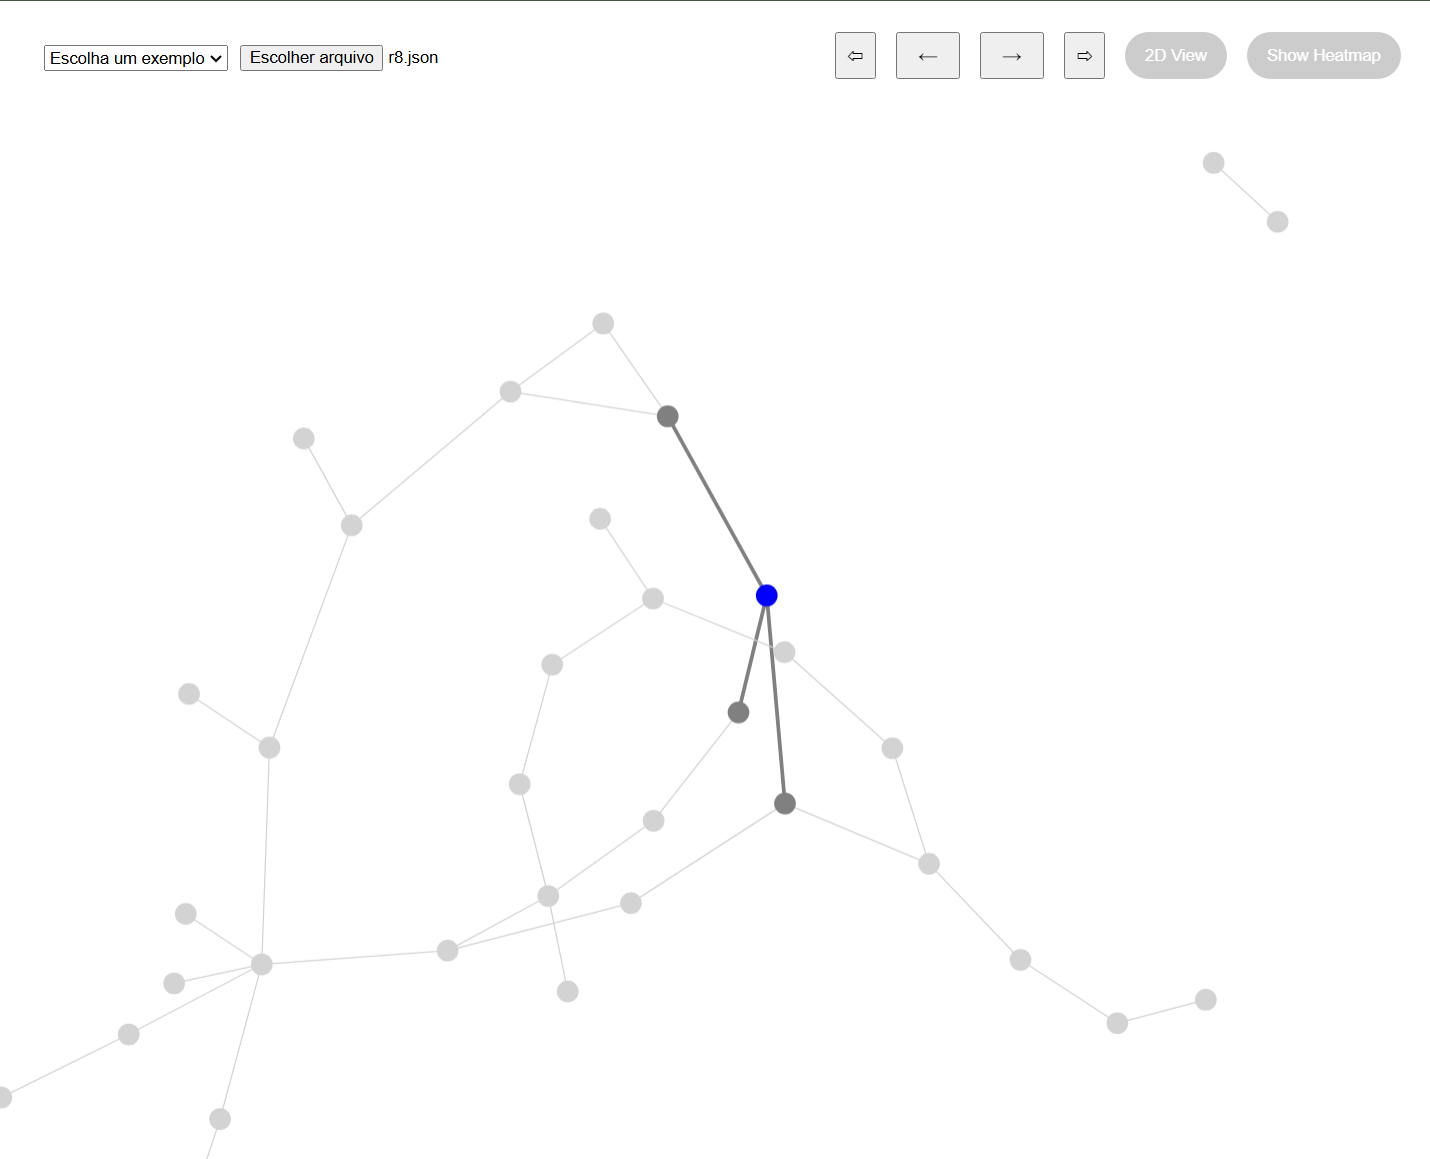
\includegraphics[width=12cm]{GrafoSteps1.png}
\caption{Passo 1 do algoritmo}
\label{fig:grafo-steps-1}
\end{figure}

\begin{figure}[!htb]
\centering
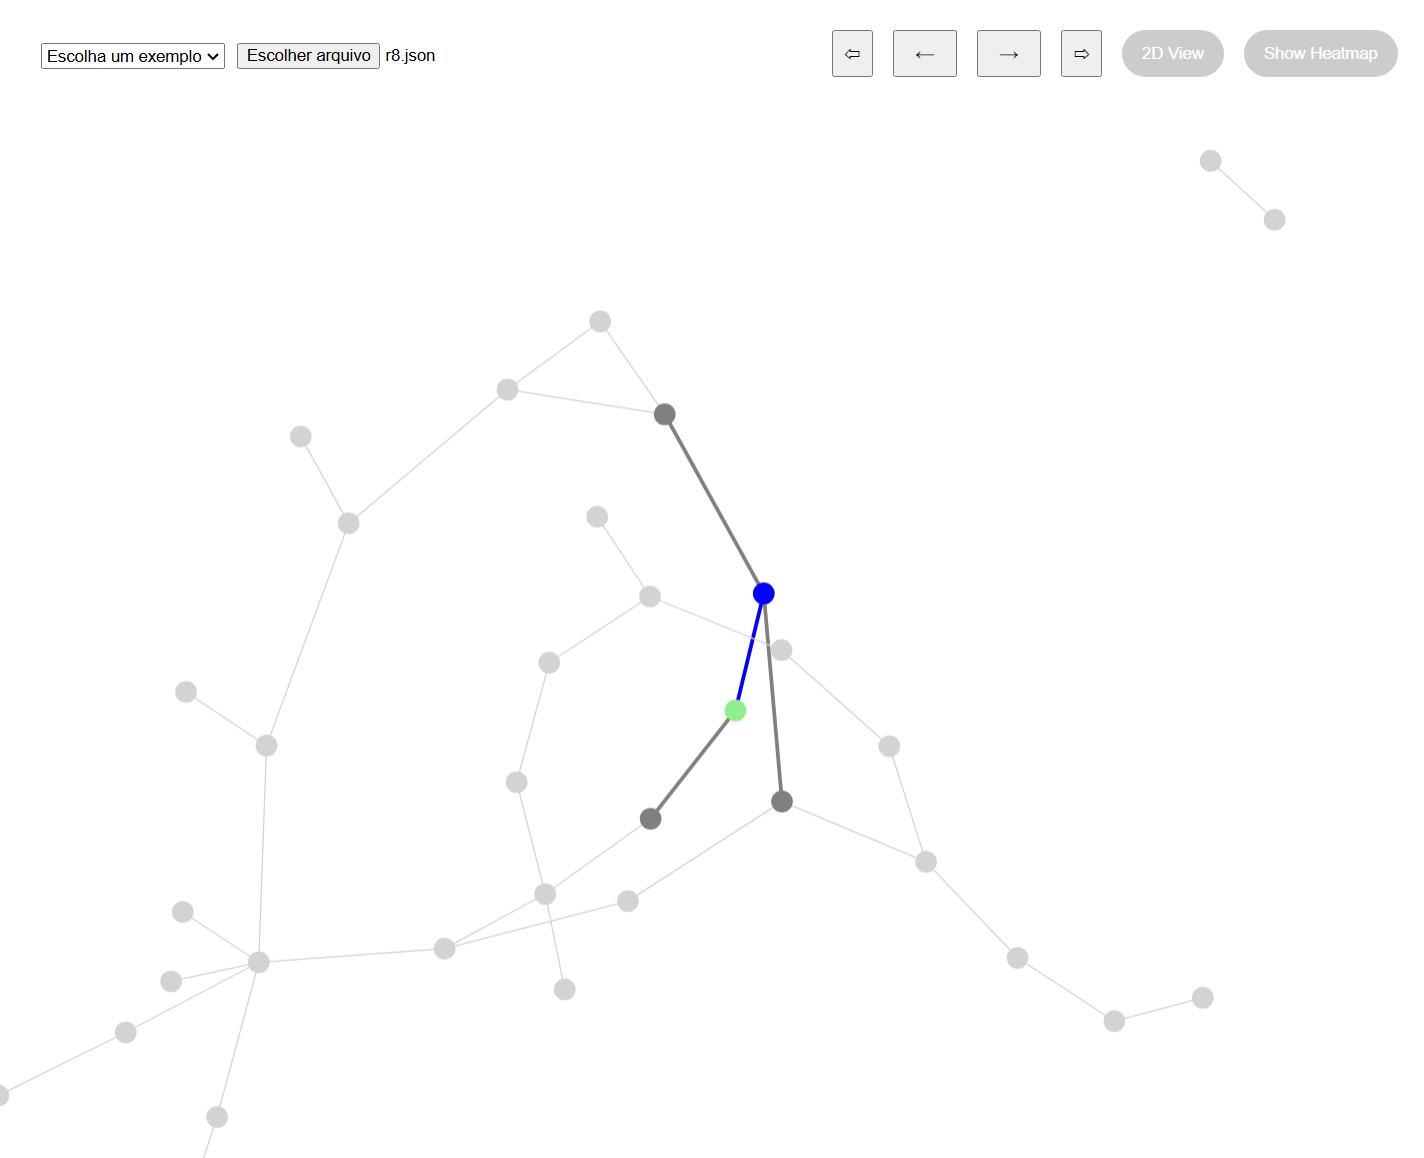
\includegraphics[width=12cm]{GrafoSteps2.png}
\caption{Passo 2 do algoritmo}
\label{fig:grafo-steps-2}
\end{figure}

\begin{figure}[!htb]
\centering
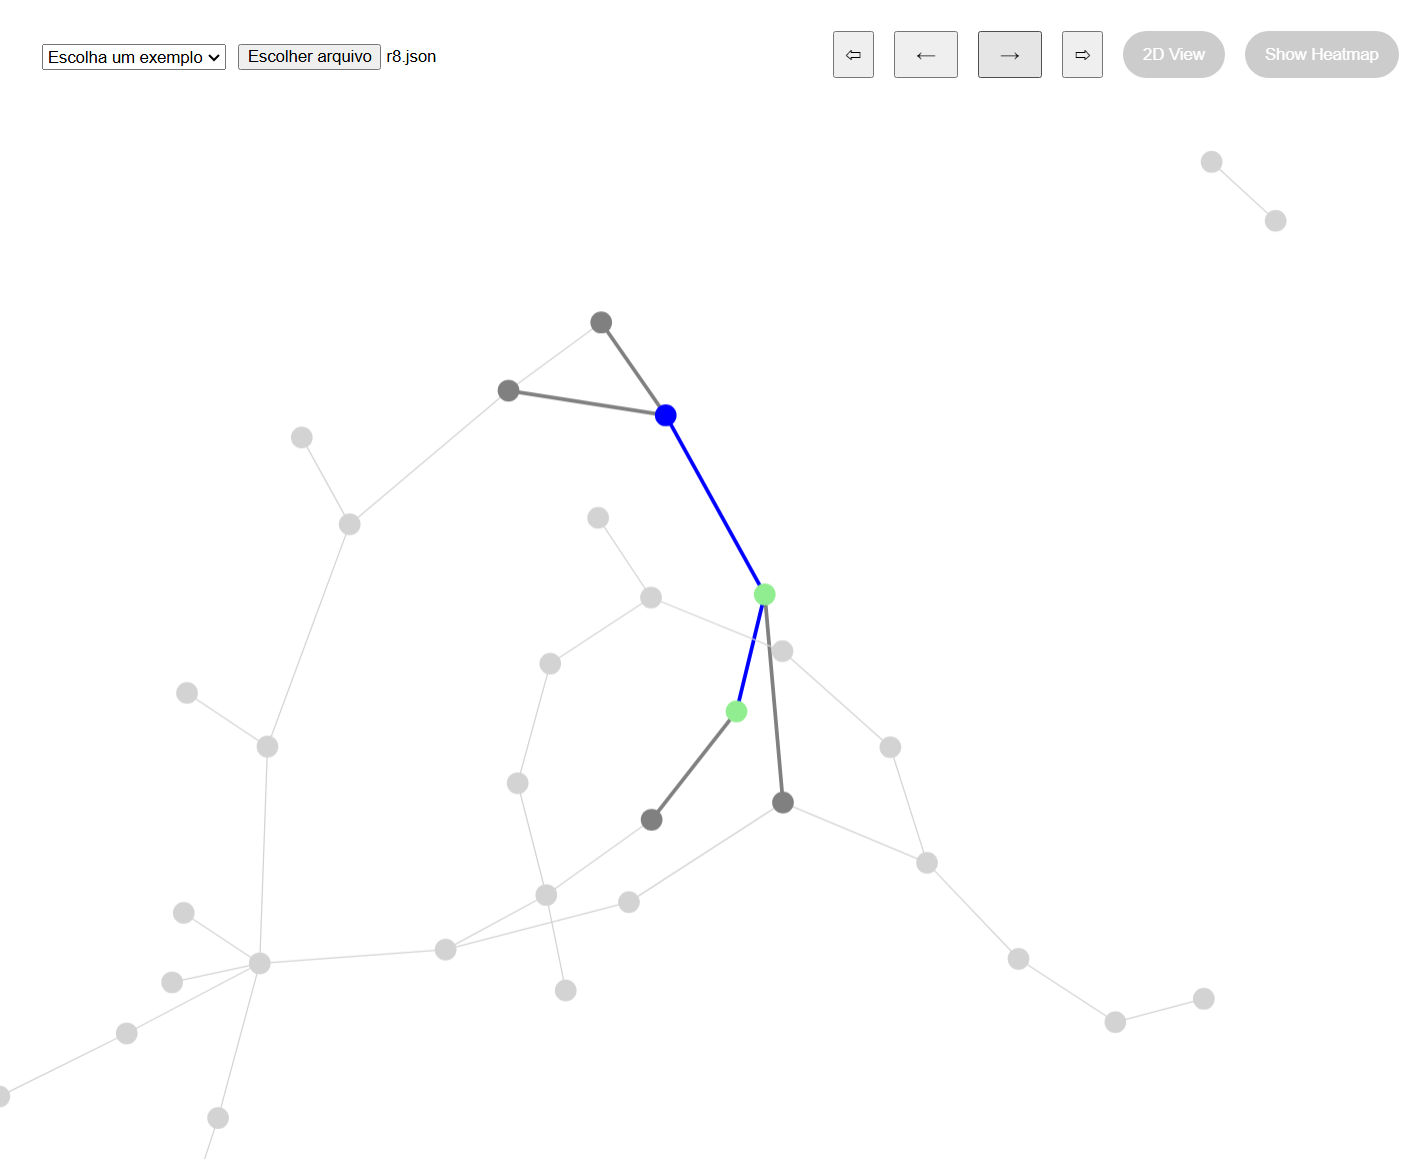
\includegraphics[width=12cm]{GrafoSteps3.png}
\caption{Passo 3 do algoritmo}
\label{fig:grafo-steps-3}
\end{figure}

\begin{figure}[!htb]
\centering
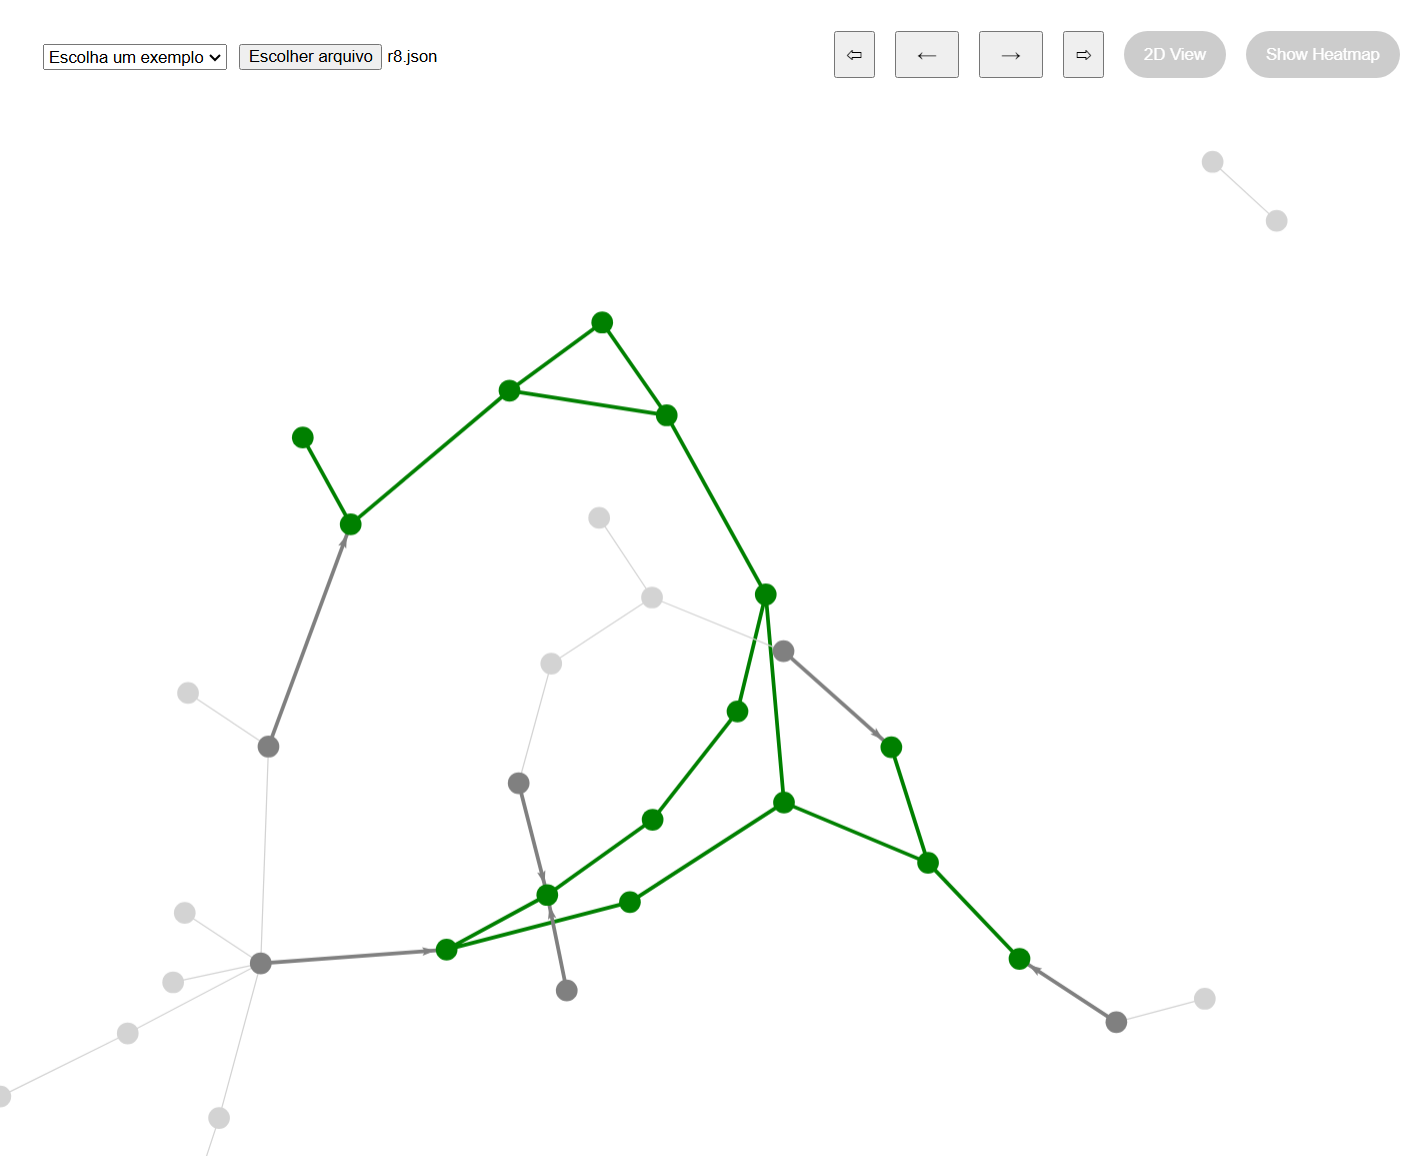
\includegraphics[width=12cm]{GrafoStepsN.png}
\caption{Passo final do algoritmo}
\label{fig:grafo-steps-n}
\end{figure}

\subsection{Mapa de calor}
É possível também ativar a visualização do mapa de calor, que colore os vértices de acordo com a quantidade de vezes que ele foi explorado pelo algoritmo.

\begin{figure}[!htb]
\centering
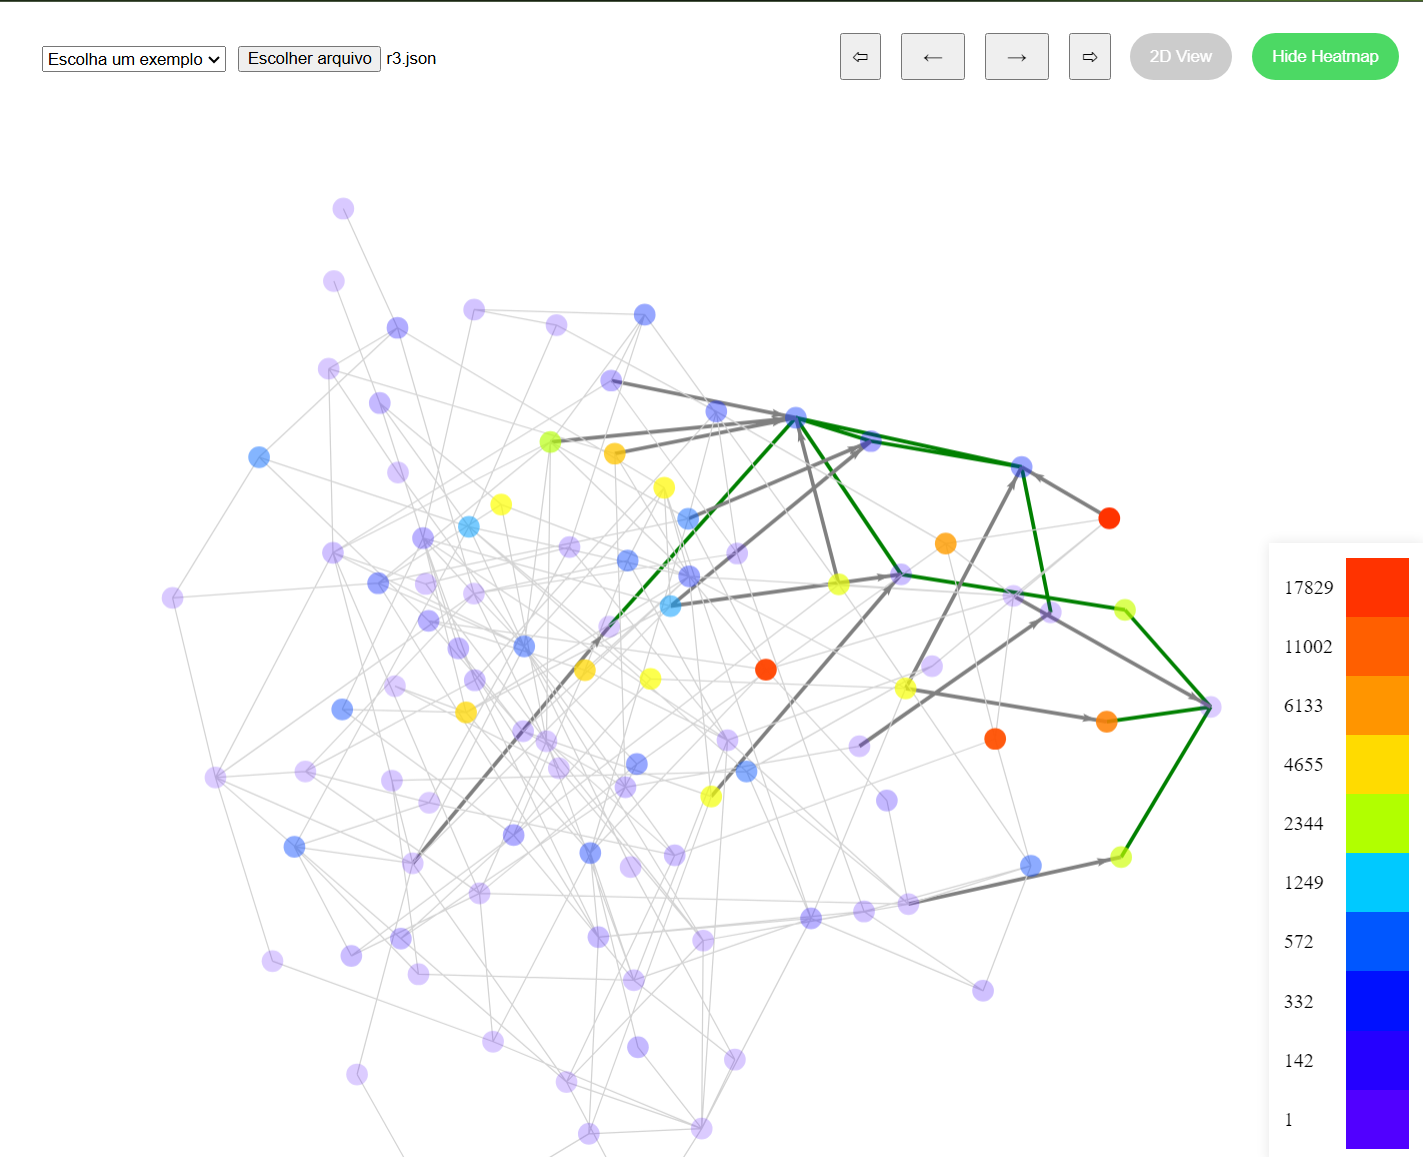
\includegraphics[width=12cm]{GrafoHeatmap.png}
\caption{Mapa de calor do grafo}
\label{fig:grafo-heatmap}
\end{figure}

Para ajudar na visualização, as cores mais frias também tem opacidade mais baixa.

Essa ferramenta em particular incentivou questionamentos interessantes a respeito da eficiência do algoritmo, como "como evitar a alta taxa de repetição de um grupo de vértices".

\chapter{Resultados e discussão}
O algoritmo originalmente estudado e a versão com as melhorias propostas foram analisadas e submetidas a um conjunto de testes para melhor ilustrar o impacto e eficiência de cada uma. Visto que o problema continua sendo NP-completo, há pouco a ser feito para valores realmente grandes, mas foi possível sim observar uma ampliação dos valores considerados "razoáveis" pelo algoritmo FPT.

Para testar o algoritmo utilizamos a função da biblioteca \texttt{networkx nx.erdos\_renyi\_graph(v,e,seed)} onde \texttt{v} é o número de vértices \texttt{e} é a probabilidade de 2 vértices formarem uma aresta, e \texttt{seed} é uma semente para geração do Grafo.

Para os testes a seguir foram fixados os seguintes seguintes parâmetros \texttt{v=30} \texttt{e=0.333} e \texttt{seed=100} e executamos para \texttt{k} variando entre \texttt{1} e \texttt{29}.

\begin{figure}[!htb]
\centering
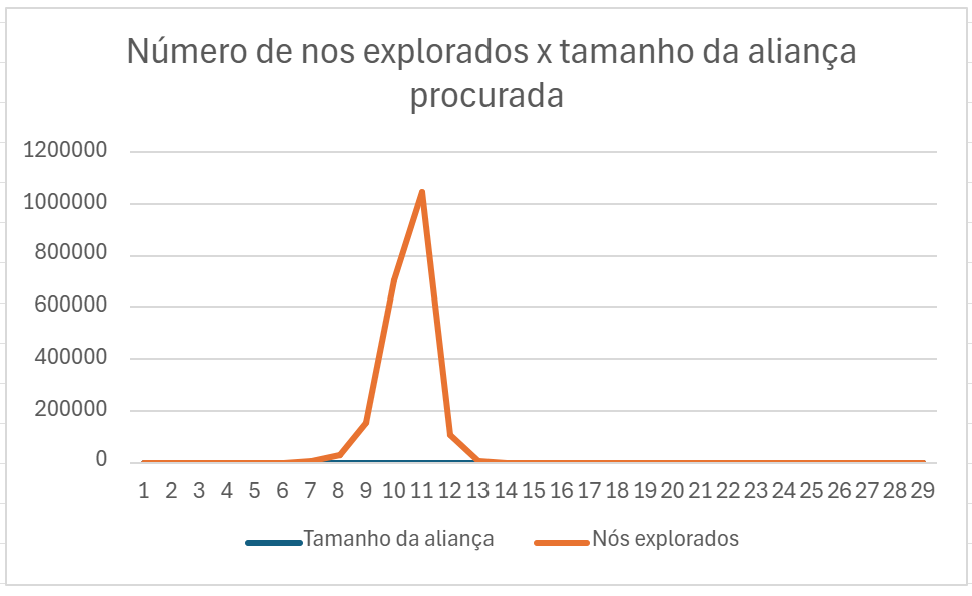
\includegraphics[width=12cm]{Execução sem repetição de conjuntos.png}
\caption{Execução do algoritmo \textbf{evitando} a repetição de conjuntos}
\label{fig:execucao-sem-repeticao}
\end{figure}

Na execução do algoritmo sem repetição de conjuntos é possível notar que o número máximo de nós explorados foi de aproximadamente 1 milhão de nós.

\begin{figure}[!htb]
\centering
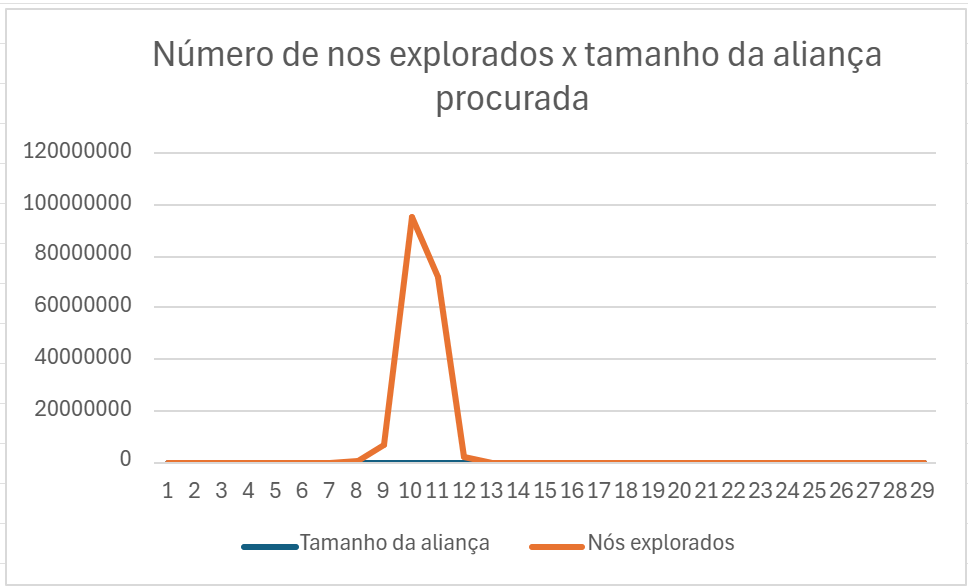
\includegraphics[width=12cm]{Execução com repetição de conjuntos.png}
\caption{Execução do algoritmo \textbf{permitindo} a repetição de conjuntos}
\label{fig:execucao-com-repeticao}
\end{figure}

Por sua vez, na execução que permite a repetição de conjuntos o número de nós explorados nesse caso saltou de 1 milhão para 100 milhões.

Salvar os conjuntos resulta em uma melhora significativa na redução do número de nós a serem explorados, porém nós traz um novo problema pois o espaço necessário para armazenar todos esses conjuntos no pior caso é $\sum_{i=0}^{k} \binom{n}{i}<2^n$, ou seja, acabamos trocando um tempo exponencial, por espaço exponencial.

Foi observado um padrão interessante na eficiência com relação ao grau médio dos vértices do grafo $d(G)$ e $k$; o número de nós explorados atinge um ápice para valores de $k$ próximos de $d(G)$ criando uma "zona difícil", e suaviza a medida que a diferença aumenta.

Para valores de $d(G)$ muito maiores que $k$ isso acontece porque o algoritmo pode descartar muitas combinações através do critério \texttt{Se v.c\_w <= k - tamanho de S:}. Essa linha garante que o próximo nó a ser expandido ao menos tem as condições de ser protegido dado o tamanho atual de $S$.

Por outro lado, valores de $k$ muito menores do que $d(G)$, foi observado uma probabilidade maior de haver uma aliança defensiva. A modificação de ordenação dos vértices de \texttt{W} com base em quantos vizinhos ele possui em $S$ e $\lfloor d(v)/2 \rfloor$, em especial, mostrou acelerar muito o processo de determinação da aliança, quando existente. Isso se deve as escolhas priorizarem a defesa dos vértices já em $S$, em prol de adições aleatórias.

Por fim, a modificação de "Evitar repetir conjuntos" mostrou-se acelerar o processo tanto no melhor caso quanto no pior, pois garante que somente novas combinações são testadas.

\chapter{Conclusão}
O estudo como um todo foi bastante produtivo dentro do tema, e possibilitou compreensão significativa do que são e como encontrar alianças defensivas. O visualizador web, como ferramenta didática, foi bastante aproveitado para a compreensão e elaboração das melhorias propostas ao algoritmo.

Também foi produtivo experimentar na prática a complexidade de um problema NP-completo e uma das ferramentas usadas para contornar esse degrau gigantesco na complexidade.

Dentre os diversos temas que podem ser abordados em discussões futuras, destacamos a implementação e análise do algoritmo proposto por \cite{Enciso2009} para encontrar Conjuntos Seguros (\textit{Secure Sets}), que segue uma abordagem FPT semelhante ao de alianças defensivas, e pode ser adaptado para o visualizador web para gerar resultados valiosos.

Outro ponto de possível expansão é o de pré-análise de grafos para a determinação de potencial de uma aliança de tamanho $k$, partindo da análise feita sobre o grau médio e a "zona difícil".
		% conclusão

%=====================================================

% ATENÇÃO:
% - o estilo da bibliografia é definido no arquivo packages.tex
% - evite usar \cite{}; prefira \citep{} e \citet{}

% base de bibliografia (arquivo .bib do BibTeX)
\bibliography{referencias}
%\bibliography{file1,file2,file3} % se tiver mais de um arquivo BibTeX

%=====================================================

% inclusão de apêndices
\appendix

% inclusão de apêndice
% \chapter{Fundamentação teórica}
A fim de seguir de forma devida com a análise do problema e do algoritmo, algumas definições teóricas são requeridas:

\section{Conceitos}

\subsection{Grafo}
Um grafo $G = (V(G), E(G))$ é um par ordenado que consiste de um conjunto de vértices $V(G)$ e um conjunto de arestas $E(G)$.

\subsection{Vértice}
Um vértice $v \in V(G)$ é um elemento básico de um grafo, representando um ponto ou nó na estrutura. O conjunto $V(G)$ é finito e contém todos os vértices do grafo.

\subsection{Aresta}
Uma aresta $e \in E(G)$ é um conjunto de dois vértices de $V(G)$. Em um grafo não direcionado, a aresta $\{u, v\}$ conecta os vértices $u$ e $v$, sem direção. Em grafos direcionados, uma aresta $(u, v)$ conecta $u$ a $v$ com uma orientação de $u$ para $v$.

\subsection{Incidência}
As extremidades de uma aresta são ditas incidentes com a aresta \cite{Bondy2008}, e vice-versa, ou seja, uma aresta $e$ é dita incidente a um vértice $v$ se está aresta se conecta a $v$ em um de seus extremos.

\subsection{Adjacência}
Dois vértices que são incidentes a uma mesma aresta são adjacentes \cite{Bondy2008}, assim como duas arestas que são incidentes a um mesmo vértice, ou seja, um par de vértices distintos $u$ e $v$ são adjacentes se possuem uma aresta que os conectam, da mesma forma que duas arestas distintas $e1$ e $e2$ são adjacentes se são incidentes a um vértice em comum.

\subsection{Vizinhança de um Vértice}
Dois vértices que são incidentes a uma aresta comum, ou seja, dois vértices adjacentes distintos são ditos vizinhos \cite{Bondy2008}. A vizinhança de um vértice $v \in V(G)$, denotada por $N(v)$, é o conjunto de todos os vértices adjacentes a $v$, ou seja, $N(v) = \{ u \in V(G) \mid \{u, v\} \in E(G) \}$ em grafos não direcionados.

\subsection{Grau de um Vértice}
O grau de um vértice $v$ em um grafo não direcionado $G$ é dado por $d(v) = |N(v)|$, ou seja, o número de arestas incidentes a $v$. Neste estudo consideramos apenas grafos não direcionados, portanto o grau de $v$ corresponde ao número de arestas total ligadas a ele.

\subsection{Subgrafo}
Um \textbf{subgrafo} de um grafo $G$ é um grafo $F$ cujos conjuntos de vértices e arestas são subconjuntos dos vértices e arestas de $G$. Formalmente, $F$ é um subgrafo de $G$ se $V(F) \subseteq V(G)$ e $E(F) \subseteq E(G)$, e a função que relaciona vértices e arestas em $F$ é a mesma que em $G$, mas restrita ao conjunto de arestas de $F$. Subgrafos podem ser formados a partir das operações de remoção de vértices e remoção de arestas.\\
Diz-se que $G$ contém $F$ ou que $F$ está contido em $G$, representado como $G \supseteq F$ ou $F \subseteq G$.

\subsection{Conectividade}
Um grafo é \textbf{conexo} se, para toda partição de seu conjunto de vértices em dois conjuntos não vazios $X$ e $Y$, existe uma aresta com uma extremidade em $X$ e a outra extremidade em $Y$, caso contrário, o grafo é desconexo. Em outras palavras, um grafo é desconexo se seu conjunto de vértices pode ser particionado em dois subconjuntos não vazios $X$ e $Y$ de modo que nenhuma aresta tenha uma extremidade em $X$ e outra em $Y$.

\subsection{Aliança Defensiva}
Um subconjunto $S \subseteq V$ é uma aliança defensiva se, para cada vértice $v \in S$, a condição a seguir é satisfeita:   $|N(v) \cap S| \geq |N(v) \setminus S|$.\\
Ou seja, para cada vértice $v$ na aliança $S$, o número de vértices adjacentes a $v$ dentro de $S$ deve ser pelo menos igual ao número de vértices adjacentes a $v$ fora de $S$.\\
Isso indica que os vértices $v$ na aliança devem possuir pelo menos tantos vértices dentro da aliança quanto fora dela.\\
Embora, formalmente, uma aliança não precise ser conexa, note que cada componente conexa de uma aliança é uma aliança por si só. Para fins deste trabalho, toda aliança encontrada deve ser \textbf{conexa}.

\section{Complexidade Computacional}
A complexidade computacional estuda a quantidade de recursos necessários para a execução de algoritmos, especialmente em termos de tempo e espaço. Em ciência da computação, a complexidade computacional é frequentemente representada usando a notação \textit{Big O}, $O(f(n))$, que descreve o crescimento da complexidade como uma função $f(n)$, onde $n$ normalmente é o tamanho da entrada, ou algum outro parâmetro relevante. Alguns exemplos de classificação de complexidade são:

\begin{itemize}
  \item $O(1)$: Constante, o tempo de execução não depende do tamanho da entrada.
  \item $O(n)$: Linear, o tempo de execução cresce proporcionalmente ao tamanho da entrada.
  \item $O(n^k)$: Polinomial, o tempo de execução cresce proporcionalmente com relação a potência $k$ constante do tamanho da entrada. Um exemplo de polinômio muito comum são os quadrados $O(n^2)$.
  \item $O(k^n)$: Exponencial, o tempo de execução cresce de forma exponencial com relação ao tamanho da entrada. No geral, é inviável para grandes entradas.
  \item $O(n!)$ Fatorial, em problemas fatoriais o tempo de execução cresce ainda mais acelerado com relação ao tamanho da entrada do que problemas exponenciais.
\end{itemize}

\subsection{Classes de Complexidade:}
Os problemas de decisão, como os envolvendo alianças, podem ser classificados em certas classes de complexidade que separam o quão viáveis é encontrar ou verificar suas soluções para entradas de larga escala. Estas classes não:

\begin{itemize}
  \item $P$ (Polinomial): Representa a classe de problemas que podem ser resolvidos em tempo polinomial, ou seja, em $O(n^k)$ para algum inteiro $k$. Em ciência da computação, problemas em $P$ são considerados tratáveis.
  \item $NP$ (Tempo polinomial não determinístico): Representa a classe de problemas para os quais, apesar de não sabermos como encontrar solução em tempo polinomial de maneira determinística, dada uma solução, ela pode ser verificada em tempo polinomial por um algoritmo determinístico. Não sabemos se todo problema em $NP$ pode ser resolvido em tempo polinomial, isto é, se $P = NP$, e esse é um dos 7 problemas do milênio que ainda estão em aberto.
  \item $NP$-completo: Representa um subconjunto de problemas em $NP$ que são, intuitivamente, tão difíceis quanto qualquer outro problema em $NP$. Para um problema ser dessa classe, são necessárias duas características:
  \begin{enumerate}
    \item Estar em $NP$, ou seja, dada uma solução, ela deve ser verificável em tempo polinomial.
    \item Ser $NP$-difícil, todo problema em $NP$ pode ser redutível a ele em tempo polinomial.\\
Em outras palavras, caso um problema de classe $NP$-completo seja resolvido em tempo polinomial, todos os outros problemas em $NP$ poderão ser resolvidos em tempo polinomial.
  \end{enumerate}
\end{itemize}

\section{O algoritmo}
Como encontrar uma aliança defensiva em um grafo é um problema NP-completo, o algoritmo FPT \cite{Enciso2009} tem como objetivo buscar por uma aliança conexa arbitrária de tamanho máximo $k$, a fim de tornar o problema tratável. Porém, neste trabalho o tamanho da aliança buscada será \textit{exatamente} $k$, pois acreditamos que o tamanho da aliança seja importante. Antes de entrar na explicação minuciosa do algoritmo, é importante explicar o que é um algoritmo FPT.

\subsection{Complexidade}
FPT (\textit{Fixed-Parameter Tractable}) é uma classe de complexidade que trata de problemas parametrizáveis (como os de complexidade exponencial) ao isolar e fixar um parâmetro específico do problema, chamado $k$, e então expressando a complexidade na forma $f(k)*p(n).$ Desta forma, $f(k)$ é a parte da complexidade que depende exclusivamente de $k$ e pode ser \textit{superpolinomial}, enquanto $p(n)$ é uma função polinomial de $n$. Sendo assim, fixar $k$ em valores pequenos nos permite abordar o algoritmo de forma mais tratável, custando muito menos tempo, a depender do tamanho de $k$.

O algoritmo usado neste estudo foi proposto por \cite{Enciso2009}, e tem complexidade $O(k^kn)$, e é uma melhora significativa de seu predecessor, que tinha complexidade $O((2k-1)^kk^2n)$. Esse é um avanço substancial, mas ainda é interessante demonstrar como problemas, mesmo parametrizados, crescem rapidamente:

\begin{table}[h]
\begin{center}
\begin{tabular}{|c|c|c|c|c|c|c|c|}
\hline
$k$ & $k^k$\\
\hline
2 & 4 \\
\hline
3 & 27 \\
\hline
4 & 256 \\
\hline
5 & 3.125 \\
\hline
6 & 46.656 \\
\hline
7 & 823.543 \\
\hline
9 & 387.420.489 \\
\hline
10 & 10.000.000.000 \\
\hline
\end{tabular}
\end{center}
\end{table}

\begin{figure}[!htb]
\centering
\includegraphics[height=12cm]{GraficoKelevK.png}
\caption{Gráfico da função $k^k$}
\label{fig:kelevk}
\end{figure}

O propósito do algoritmo então é garantir que o tempo possa ser diminuído de acordo com $k$, sem que seja necessário executar para todo $n-k$ restante.

\subsection{Explicação}
O algoritmo é dividido em duas funções principais, a \texttt{main} e a \texttt{defensiveAlliance}. A \texttt{main} recebe como entrada um Grafo $G$ e o tamanho da aliança desejada, um inteiro positivo $k$. De forma intuitiva, a abordagem do algoritmo é partir de um vértice do grafo por vez e olhar sua vizinhança numa tentativa de expandi-lo até formar uma aliança defensiva de tamanho $k$, ou todos os vértices terem servido de raiz da expansão.

\lstset{ 
  deletekeywords={do}  
}

\begin{lstlisting}[escapeinside={(*}{*)}]
Main(G,k)
	Para cada vértice v de G:
		v.c_w <- (*$\ceil{\frac{d(v)}{2}}$*).
	Para cada vértice v de G:
		inicia uma aliança S <- {v}.
		aliança_encontrada <- DefensiveAlliance(S).
		Se aliança_encontrada:
			retorne aliança_encontrada.
		retira v de S
		soma 1 ao c_w de v.
			
	retorne "Sem aliança";
\end{lstlisting}

O papel da função \texttt{main} é garantir que todos os vértices foram usados como raiz da expansão. Para isso, primeiro é definido o \texttt{c\_w}, que serve para verificar se o vértice está protegido dentro da aliança \texttt{S}. De início, ela é definida com o número de vizinhos necessários dentro de $S$ para que ele esteja defendido, e então será aumentada ou diminuida conforme se adiciona ou remove seus vizinhos a $S$.

Isso também faz parte da condição de sucesso da busca, ou seja, quando todos os vértices de \texttt{S} estiverem protegidos (\texttt{c\_w <= 0}) então uma aliança defensiva foi formada.

A seguir, a \texttt{main} chama a função \texttt{defensiveAlliance} para verificar se \texttt{S} é, ou pode ser expandida até, uma aliança defensiva de tamanho \texttt{k}.

\begin{lstlisting}[escapeinside={(*}{*)}]
DefensiveAlliance(G, S, k)
	inicia v <- vértice de maior c_w em S.
	Se v.c_w <= 0 e tamanho de S == k:
		devolve S.
		
	Se v.c_w <= k - tamanho de S: 
		inicia t <- 1 + metade dos vizinhos de w.
		inicia o conjunto W <- t vizinhos de w que não pertencem a S.
		Para cada vértice w em W:
			S <- S + w.
			Para cada vizinho x de w em S:
				subtrai 1 do c_w de x e de w.
			aliança_encontrada <- DefensiveAlliance(G, S, k)
			Se aliança_encontrada:
				Devolve aliança_encontrada.
			Para cada vizinho x de w em S:
				soma 1 ao c_w de x e de w.
			Retira w de S.
			
	Retorne NULL;
\end{lstlisting}

No início de \texttt{defensiveAlliance} o algoritmo escolhe o vértice de maior \texttt{c\_w} em \texttt{S},  que seria o vértice mais vulnerável da aliança. Esse vértice serve para tanto verificar se \texttt{S} se tornou uma aliança quanto como ponto de expansão a fim de incluir novos vértices.

A seguir, o algoritmo verifica se há espaço em \texttt{S} para os \texttt{c\_w} vizinhos necessários serem adicionados, ou seja, para que \texttt{w} seja defendido dentro da restrição do tamanho máximo \texttt{k}. Essa verificação funciona de modo semelhante a uma heurística de busca, poupando tempo ao evitar vértices que não podem ser defendidos posteriormente.

\subsection{Lema 14}
Uma parte importante do funcionamento do algoritmo é o lema 14 de \cite{Enciso2009}. Assuma que $S \subseteq V$ é estendível para uma aliança defensiva S', onde $|S| <|S'| = k$ então, para qualquer vértice desprotegido $w \in S$, $|S' \cap (N[w] - S|) \ge c_w$.\\
Em outras palavras se $S$ é estendível e $w$ é um vértice desprotegido de $S$ então $c_w$ é o número de vizinhos de $w$ fora de $S$ que é necessário para proteger $w$ em $S$.

Esse lema é o que podemos considerar como o núcleo do algoritmo, pois ele nos garante também que para qualquer subconjunto $W \subseteq N[w] - S$ com $t = \lfloor \frac{d_w}{2} \rfloor + 1$  vértices contém ao menos um vértice $w_i$ para o qual $S \cup {w_i}$ é estendível se e somente se S é estendível.

\subsection{Evitando repetir conjuntos}
Observando o comportamento do algoritmo no visualizador web foi possível notar que um comportamento pouco eficiente: o critério de expansão de $S$ (destacado a seguir) abre margem pra repetir várias vezes a mesma combinação de vértices, levando, principalmente em grafos de grande quantidade de vértices, a muito esforço improdutivo.

\begin{lstlisting}
DefensiveAlliance(G, S, k)
	inicia v <- vértice de maior c_w em S.
\end{lstlisting}

Pensando nisso a equipe elaborou uma solução que armazena todas as combinações já analisadas anteriormente e impede de que novas iterações com elas sejam geradas, cortando toda a sub-árvore subsequente. Isso é feito com a criação de um dicionário e a marcação única de cada combinação:

\begin{lstlisting}
inicia combinacoes <- dicionário vazio
\end{lstlisting}

\begin{lstlisting}
DefensiveAlliance(G, S, k)
[...]
	Para cada vértice w em W:
		S <- S + w.
		
		comb_id <- identificadores de S de forma ordenada.
		Se existe combinacoes[comb_id]:
			Retira w de S.
			pula para o próximo vértice.
		Caso contrário:	
			cria combinacoes[comb_id].

		Para cada vizinho x de w em S:
			subtrai 1 do c_w de x e de w.
		aliança_encontrada <- DefensiveAlliance(G, S, k)
[...]
\end{lstlisting}

Caso não exista uma entrada da combinação no dicionário, cria-se uma e a instância corrente de \texttt{S} é analisada. Caso contrário, a instância é ignorada, podando todas as sub-árvores subsequentes. A complexidade de tempo é se resume a ordenação de, no máximo, $k-1$ elementos, e ao acesso e escrita no dicionário. Ambos são ofuscados pela complexidade geral.

Por outro lado, há um custo sério em termos de espaço. No pior caso, de não haver aliança e o algoritmo analisar todos os vértices e $k=n$, a combinação ocupa espaço $O(2^n)$, que corresponde a guardar todas as combinações de $n$ vértices, variando de tamanho $1$ até $n$. Isso pode ser mitigado ao limitar o tamanho das combinações armazenadas para a região crítica que vai ser repetida mais vezes. A análise desta região está na seção sobre Resultados e discussão.

Quanto ao desempenho, esta técnica permite ao algoritmo poupar muito tempo ao "amortizar" o custo $k^k$ ao longo de várias iterações, pois, como nenhuma combinação é repetida, quanto mais exploradas são as combinações dos vértices, menos combinações existem para serem analisadas.

\subsection{Priorização dos vértices expostos}
\begin{lstlisting}
DefensiveAlliance(G, S, k)
	inicia v <- vértice de maior c_w em S.
\end{lstlisting}

Ao iniciarmos $DefensiveAlliance(G,S,k)$ atribuindo $v$ o vértice em $W$ com maior $c_w$ nós garantimos que a maior prioridade em cada chamada recursiva da função é proteger o vértice mais "exposto".

Assim obtemos também um critério de parada consistente, ou seja, quando o vértice com maior $c_w$ ter $c_w \le 0$ e $|S| = k$, teremos duas informações fundamentais sobre o contexto da execução:\\
1 - Se $c_w \le 0$, então todos os vértices em $S$ estão protegidos.\\
2 - Se $|S|=k$, encontramos a aliança defensiva procurada.

\chapter{Metodologia}
O projeto é composto por duas partes principais: algoritmos de busca implementados em Python e um visualizador web criado para exibir os passos deste algoritmo. As partes funcionam de forma independente, sendo conectadas apenas pelo formato de entrada e saída dos programas.

\section{Algoritmo em Python}
A implementação do algoritmo proposto por \cite{Enciso2009} foi feita em Python e consta completa no Apêndice 1.

Nesta implementação foi utilizada a estrutura de dados da biblioteca \textit{Networkx} para manipulação dos grafos, e, no mais, estruturada de forma semelhante ao algoritmo teórico, com a exceção do uso de uma estrutura de pilha para substituir a chamada recursiva.

Além do resultado final, o programa possibilita o retorno da aliança em formato JSON, com as características utilizadas no visualizador web. Essas características permitem a visualização passo a passo dos nós expandidos pelo algoritmo, e consistem do conjunto $W$ a cada iteração da função \texttt{DefensiveAlliance}.

Há também \textit{flags} para mostrar a quantidade de nós expandidos, para gerar um grafo aleatório segundo uma densidade especificada, e para alterar o comportamento da busca, como retornar a primeira aliança encontrada independente do tamanho.

\section{Visualizador web}
O projeto web foi desenvolvido com Typescript e React, e sua proposta é fornecer uma visualização passo-a-passo do algoritmo e do grafo de entrada. Assim como o algoritmo de busca, o visualizador pode ser encontrado no repositório que se encontra nas referências.

Para montar a visualização é necessário que seja fornecido como entrada um grafo disposto em formato JSON, contando com dois conjuntos extras de dados que são a aliança encontrada, caso exista, e um vetor de \textit{steps}, que contém o conjunto $W$ no dado \textit{passo} da iteração.

Munido destas informações, o visualizador organiza os dados internamente para melhorar o desempenho e a decisão de cada caraterística visual do grafo e então personaliza uma \textit{view} HTML, dada pela biblioteca 3d-force-graph \cite{HassanShafique2004}, que cuida da renderização e simulação física do grafo.

Dentre as funcionalidades, vale destacar duas principais: a visualização do conjunto $S$ a cada etapa do algoritmo e o mapa de calor dos nós explorados. O mapa de calor é a coloração dos vértices do grafo seguindo a regra de que, quanto mais visitado um vértice durante a execução do algoritmo, mais quente é a cor usada; os nós mais quentes tem cores próximas do vermelho, e os mais frios, mais próximas do azul.

\subsection{Visualização por passos}
Ao carregar um grafo com o conjunto de passos, é possível navegar por cada um deles. Em um certo passo, os vértices e arestas da fronteira de $S$ são desenhados com uma cor cinza escura, os além da fronteira tem cor cinza claro, e os vértices dentro de $S$ ficam coloridos com a cor

\begin{itemize}
  \item azul, se estiverem desprotegidos;
  \item ou verde, se estiverem devidamente protegidos.
\end{itemize}

Ao finalizar o algoritmo e desenhar a aliança, ela é colorida de verde escuro.

As figuras a seguir são de uma busca por uma aliança de tamanho $k = 15$ em um grafo de $v=50$ vértices e $e=40$ arestas. O algoritmo começa com $S$ contendo o vértice colorido de azul.

\begin{figure}[!htb]
\centering
\includegraphics[width=12cm]{GrafoSteps1.png}
\caption{Passo 1 do algoritmo}
\label{fig:grafo-steps-1}
\end{figure}

\begin{figure}[!htb]
\centering
\includegraphics[width=12cm]{GrafoSteps2.png}
\caption{Passo 2 do algoritmo}
\label{fig:grafo-steps-2}
\end{figure}

\begin{figure}[!htb]
\centering
\includegraphics[width=12cm]{GrafoSteps3.png}
\caption{Passo 3 do algoritmo}
\label{fig:grafo-steps-3}
\end{figure}

\begin{figure}[!htb]
\centering
\includegraphics[width=12cm]{GrafoStepsN.png}
\caption{Passo final do algoritmo}
\label{fig:grafo-steps-n}
\end{figure}

\subsection{Mapa de calor}
É possível também ativar a visualização do mapa de calor, que colore os vértices de acordo com a quantidade de vezes que ele foi explorado pelo algoritmo.

\begin{figure}[!htb]
\centering
\includegraphics[width=12cm]{GrafoHeatmap.png}
\caption{Mapa de calor do grafo}
\label{fig:grafo-heatmap}
\end{figure}

Para ajudar na visualização, as cores mais frias também tem opacidade mais baixa.

Essa ferramenta em particular incentivou questionamentos interessantes a respeito da eficiência do algoritmo, como "como evitar a alta taxa de repetição de um grupo de vértices".

\chapter{Resultados e discussão}
O algoritmo originalmente estudado e a versão com as melhorias propostas foram analisadas e submetidas a um conjunto de testes para melhor ilustrar o impacto e eficiência de cada uma. Visto que o problema continua sendo NP-completo, há pouco a ser feito para valores realmente grandes, mas foi possível sim observar uma ampliação dos valores considerados "razoáveis" pelo algoritmo FPT.

Para testar o algoritmo utilizamos a função da biblioteca \texttt{networkx nx.erdos\_renyi\_graph(v,e,seed)} onde \texttt{v} é o número de vértices \texttt{e} é a probabilidade de 2 vértices formarem uma aresta, e \texttt{seed} é uma semente para geração do Grafo.

Para os testes a seguir foram fixados os seguintes seguintes parâmetros \texttt{v=30} \texttt{e=0.333} e \texttt{seed=100} e executamos para \texttt{k} variando entre \texttt{1} e \texttt{29}.

\begin{figure}[!htb]
\centering
\includegraphics[width=12cm]{Execução sem repetição de conjuntos.png}
\caption{Execução do algoritmo \textbf{evitando} a repetição de conjuntos}
\label{fig:execucao-sem-repeticao}
\end{figure}

Na execução do algoritmo sem repetição de conjuntos é possível notar que o número máximo de nós explorados foi de aproximadamente 1 milhão de nós.

\begin{figure}[!htb]
\centering
\includegraphics[width=12cm]{Execução com repetição de conjuntos.png}
\caption{Execução do algoritmo \textbf{permitindo} a repetição de conjuntos}
\label{fig:execucao-com-repeticao}
\end{figure}

Por sua vez, na execução que permite a repetição de conjuntos o número de nós explorados nesse caso saltou de 1 milhão para 100 milhões.

Salvar os conjuntos resulta em uma melhora significativa na redução do número de nós a serem explorados, porém nós traz um novo problema pois o espaço necessário para armazenar todos esses conjuntos no pior caso é $\sum_{i=0}^{k} \binom{n}{i}<2^n$, ou seja, acabamos trocando um tempo exponencial, por espaço exponencial.

Foi observado um padrão interessante na eficiência com relação ao grau médio dos vértices do grafo $d(G)$ e $k$; o número de nós explorados atinge um ápice para valores de $k$ próximos de $d(G)$ criando uma "zona difícil", e suaviza a medida que a diferença aumenta.

Para valores de $d(G)$ muito maiores que $k$ isso acontece porque o algoritmo pode descartar muitas combinações através do critério \texttt{Se v.c\_w <= k - tamanho de S:}. Essa linha garante que o próximo nó a ser expandido ao menos tem as condições de ser protegido dado o tamanho atual de $S$.

Por outro lado, valores de $k$ muito menores do que $d(G)$, foi observado uma probabilidade maior de haver uma aliança defensiva. A modificação de ordenação dos vértices de \texttt{W} com base em quantos vizinhos ele possui em $S$ e $\lfloor d(v)/2 \rfloor$, em especial, mostrou acelerar muito o processo de determinação da aliança, quando existente. Isso se deve as escolhas priorizarem a defesa dos vértices já em $S$, em prol de adições aleatórias.

Por fim, a modificação de "Evitar repetir conjuntos" mostrou-se acelerar o processo tanto no melhor caso quanto no pior, pois garante que somente novas combinações são testadas.

\chapter{Conclusão}
O estudo como um todo foi bastante produtivo dentro do tema, e possibilitou compreensão significativa do que são e como encontrar alianças defensivas. O visualizador web, como ferramenta didática, foi bastante aproveitado para a compreensão e elaboração das melhorias propostas ao algoritmo.

Também foi produtivo experimentar na prática a complexidade de um problema NP-completo e uma das ferramentas usadas para contornar esse degrau gigantesco na complexidade.

Dentre os diversos temas que podem ser abordados em discussões futuras, destacamos a implementação e análise do algoritmo proposto por \cite{Enciso2009} para encontrar Conjuntos Seguros (\textit{Secure Sets}), que segue uma abordagem FPT semelhante ao de alianças defensivas, e pode ser adaptado para o visualizador web para gerar resultados valiosos.

Outro ponto de possível expansão é o de pré-análise de grafos para a determinação de potencial de uma aliança de tamanho $k$, partindo da análise feita sobre o grau médio e a "zona difícil".


% inclusão de apêndice
% \chapter{Fundamentação teórica}
A fim de seguir de forma devida com a análise do problema e do algoritmo, algumas definições teóricas são requeridas:

\section{Conceitos}

\subsection{Grafo}
Um grafo $G = (V(G), E(G))$ é um par ordenado que consiste de um conjunto de vértices $V(G)$ e um conjunto de arestas $E(G)$.

\subsection{Vértice}
Um vértice $v \in V(G)$ é um elemento básico de um grafo, representando um ponto ou nó na estrutura. O conjunto $V(G)$ é finito e contém todos os vértices do grafo.

\subsection{Aresta}
Uma aresta $e \in E(G)$ é um conjunto de dois vértices de $V(G)$. Em um grafo não direcionado, a aresta $\{u, v\}$ conecta os vértices $u$ e $v$, sem direção. Em grafos direcionados, uma aresta $(u, v)$ conecta $u$ a $v$ com uma orientação de $u$ para $v$.

\subsection{Incidência}
As extremidades de uma aresta são ditas incidentes com a aresta \cite{Bondy2008}, e vice-versa, ou seja, uma aresta $e$ é dita incidente a um vértice $v$ se está aresta se conecta a $v$ em um de seus extremos.

\subsection{Adjacência}
Dois vértices que são incidentes a uma mesma aresta são adjacentes \cite{Bondy2008}, assim como duas arestas que são incidentes a um mesmo vértice, ou seja, um par de vértices distintos $u$ e $v$ são adjacentes se possuem uma aresta que os conectam, da mesma forma que duas arestas distintas $e1$ e $e2$ são adjacentes se são incidentes a um vértice em comum.

\subsection{Vizinhança de um Vértice}
Dois vértices que são incidentes a uma aresta comum, ou seja, dois vértices adjacentes distintos são ditos vizinhos \cite{Bondy2008}. A vizinhança de um vértice $v \in V(G)$, denotada por $N(v)$, é o conjunto de todos os vértices adjacentes a $v$, ou seja, $N(v) = \{ u \in V(G) \mid \{u, v\} \in E(G) \}$ em grafos não direcionados.

\subsection{Grau de um Vértice}
O grau de um vértice $v$ em um grafo não direcionado $G$ é dado por $d(v) = |N(v)|$, ou seja, o número de arestas incidentes a $v$. Neste estudo consideramos apenas grafos não direcionados, portanto o grau de $v$ corresponde ao número de arestas total ligadas a ele.

\subsection{Subgrafo}
Um \textbf{subgrafo} de um grafo $G$ é um grafo $F$ cujos conjuntos de vértices e arestas são subconjuntos dos vértices e arestas de $G$. Formalmente, $F$ é um subgrafo de $G$ se $V(F) \subseteq V(G)$ e $E(F) \subseteq E(G)$, e a função que relaciona vértices e arestas em $F$ é a mesma que em $G$, mas restrita ao conjunto de arestas de $F$. Subgrafos podem ser formados a partir das operações de remoção de vértices e remoção de arestas.\\
Diz-se que $G$ contém $F$ ou que $F$ está contido em $G$, representado como $G \supseteq F$ ou $F \subseteq G$.

\subsection{Conectividade}
Um grafo é \textbf{conexo} se, para toda partição de seu conjunto de vértices em dois conjuntos não vazios $X$ e $Y$, existe uma aresta com uma extremidade em $X$ e a outra extremidade em $Y$, caso contrário, o grafo é desconexo. Em outras palavras, um grafo é desconexo se seu conjunto de vértices pode ser particionado em dois subconjuntos não vazios $X$ e $Y$ de modo que nenhuma aresta tenha uma extremidade em $X$ e outra em $Y$.

\subsection{Aliança Defensiva}
Um subconjunto $S \subseteq V$ é uma aliança defensiva se, para cada vértice $v \in S$, a condição a seguir é satisfeita:   $|N(v) \cap S| \geq |N(v) \setminus S|$.\\
Ou seja, para cada vértice $v$ na aliança $S$, o número de vértices adjacentes a $v$ dentro de $S$ deve ser pelo menos igual ao número de vértices adjacentes a $v$ fora de $S$.\\
Isso indica que os vértices $v$ na aliança devem possuir pelo menos tantos vértices dentro da aliança quanto fora dela.\\
Embora, formalmente, uma aliança não precise ser conexa, note que cada componente conexa de uma aliança é uma aliança por si só. Para fins deste trabalho, toda aliança encontrada deve ser \textbf{conexa}.

\section{Complexidade Computacional}
A complexidade computacional estuda a quantidade de recursos necessários para a execução de algoritmos, especialmente em termos de tempo e espaço. Em ciência da computação, a complexidade computacional é frequentemente representada usando a notação \textit{Big O}, $O(f(n))$, que descreve o crescimento da complexidade como uma função $f(n)$, onde $n$ normalmente é o tamanho da entrada, ou algum outro parâmetro relevante. Alguns exemplos de classificação de complexidade são:

\begin{itemize}
  \item $O(1)$: Constante, o tempo de execução não depende do tamanho da entrada.
  \item $O(n)$: Linear, o tempo de execução cresce proporcionalmente ao tamanho da entrada.
  \item $O(n^k)$: Polinomial, o tempo de execução cresce proporcionalmente com relação a potência $k$ constante do tamanho da entrada. Um exemplo de polinômio muito comum são os quadrados $O(n^2)$.
  \item $O(k^n)$: Exponencial, o tempo de execução cresce de forma exponencial com relação ao tamanho da entrada. No geral, é inviável para grandes entradas.
  \item $O(n!)$ Fatorial, em problemas fatoriais o tempo de execução cresce ainda mais acelerado com relação ao tamanho da entrada do que problemas exponenciais.
\end{itemize}

\subsection{Classes de Complexidade:}
Os problemas de decisão, como os envolvendo alianças, podem ser classificados em certas classes de complexidade que separam o quão viáveis é encontrar ou verificar suas soluções para entradas de larga escala. Estas classes não:

\begin{itemize}
  \item $P$ (Polinomial): Representa a classe de problemas que podem ser resolvidos em tempo polinomial, ou seja, em $O(n^k)$ para algum inteiro $k$. Em ciência da computação, problemas em $P$ são considerados tratáveis.
  \item $NP$ (Tempo polinomial não determinístico): Representa a classe de problemas para os quais, apesar de não sabermos como encontrar solução em tempo polinomial de maneira determinística, dada uma solução, ela pode ser verificada em tempo polinomial por um algoritmo determinístico. Não sabemos se todo problema em $NP$ pode ser resolvido em tempo polinomial, isto é, se $P = NP$, e esse é um dos 7 problemas do milênio que ainda estão em aberto.
  \item $NP$-completo: Representa um subconjunto de problemas em $NP$ que são, intuitivamente, tão difíceis quanto qualquer outro problema em $NP$. Para um problema ser dessa classe, são necessárias duas características:
  \begin{enumerate}
    \item Estar em $NP$, ou seja, dada uma solução, ela deve ser verificável em tempo polinomial.
    \item Ser $NP$-difícil, todo problema em $NP$ pode ser redutível a ele em tempo polinomial.\\
Em outras palavras, caso um problema de classe $NP$-completo seja resolvido em tempo polinomial, todos os outros problemas em $NP$ poderão ser resolvidos em tempo polinomial.
  \end{enumerate}
\end{itemize}

\section{O algoritmo}
Como encontrar uma aliança defensiva em um grafo é um problema NP-completo, o algoritmo FPT \cite{Enciso2009} tem como objetivo buscar por uma aliança conexa arbitrária de tamanho máximo $k$, a fim de tornar o problema tratável. Porém, neste trabalho o tamanho da aliança buscada será \textit{exatamente} $k$, pois acreditamos que o tamanho da aliança seja importante. Antes de entrar na explicação minuciosa do algoritmo, é importante explicar o que é um algoritmo FPT.

\subsection{Complexidade}
FPT (\textit{Fixed-Parameter Tractable}) é uma classe de complexidade que trata de problemas parametrizáveis (como os de complexidade exponencial) ao isolar e fixar um parâmetro específico do problema, chamado $k$, e então expressando a complexidade na forma $f(k)*p(n).$ Desta forma, $f(k)$ é a parte da complexidade que depende exclusivamente de $k$ e pode ser \textit{superpolinomial}, enquanto $p(n)$ é uma função polinomial de $n$. Sendo assim, fixar $k$ em valores pequenos nos permite abordar o algoritmo de forma mais tratável, custando muito menos tempo, a depender do tamanho de $k$.

O algoritmo usado neste estudo foi proposto por \cite{Enciso2009}, e tem complexidade $O(k^kn)$, e é uma melhora significativa de seu predecessor, que tinha complexidade $O((2k-1)^kk^2n)$. Esse é um avanço substancial, mas ainda é interessante demonstrar como problemas, mesmo parametrizados, crescem rapidamente:

\begin{table}[h]
\begin{center}
\begin{tabular}{|c|c|c|c|c|c|c|c|}
\hline
$k$ & $k^k$\\
\hline
2 & 4 \\
\hline
3 & 27 \\
\hline
4 & 256 \\
\hline
5 & 3.125 \\
\hline
6 & 46.656 \\
\hline
7 & 823.543 \\
\hline
9 & 387.420.489 \\
\hline
10 & 10.000.000.000 \\
\hline
\end{tabular}
\end{center}
\end{table}

\begin{figure}[!htb]
\centering
\includegraphics[height=12cm]{GraficoKelevK.png}
\caption{Gráfico da função $k^k$}
\label{fig:kelevk}
\end{figure}

O propósito do algoritmo então é garantir que o tempo possa ser diminuído de acordo com $k$, sem que seja necessário executar para todo $n-k$ restante.

\subsection{Explicação}
O algoritmo é dividido em duas funções principais, a \texttt{main} e a \texttt{defensiveAlliance}. A \texttt{main} recebe como entrada um Grafo $G$ e o tamanho da aliança desejada, um inteiro positivo $k$. De forma intuitiva, a abordagem do algoritmo é partir de um vértice do grafo por vez e olhar sua vizinhança numa tentativa de expandi-lo até formar uma aliança defensiva de tamanho $k$, ou todos os vértices terem servido de raiz da expansão.

\lstset{ 
  deletekeywords={do}  
}

\begin{lstlisting}[escapeinside={(*}{*)}]
Main(G,k)
	Para cada vértice v de G:
		v.c_w <- (*$\ceil{\frac{d(v)}{2}}$*).
	Para cada vértice v de G:
		inicia uma aliança S <- {v}.
		aliança_encontrada <- DefensiveAlliance(S).
		Se aliança_encontrada:
			retorne aliança_encontrada.
		retira v de S
		soma 1 ao c_w de v.
			
	retorne "Sem aliança";
\end{lstlisting}

O papel da função \texttt{main} é garantir que todos os vértices foram usados como raiz da expansão. Para isso, primeiro é definido o \texttt{c\_w}, que serve para verificar se o vértice está protegido dentro da aliança \texttt{S}. De início, ela é definida com o número de vizinhos necessários dentro de $S$ para que ele esteja defendido, e então será aumentada ou diminuida conforme se adiciona ou remove seus vizinhos a $S$.

Isso também faz parte da condição de sucesso da busca, ou seja, quando todos os vértices de \texttt{S} estiverem protegidos (\texttt{c\_w <= 0}) então uma aliança defensiva foi formada.

A seguir, a \texttt{main} chama a função \texttt{defensiveAlliance} para verificar se \texttt{S} é, ou pode ser expandida até, uma aliança defensiva de tamanho \texttt{k}.

\begin{lstlisting}[escapeinside={(*}{*)}]
DefensiveAlliance(G, S, k)
	inicia v <- vértice de maior c_w em S.
	Se v.c_w <= 0 e tamanho de S == k:
		devolve S.
		
	Se v.c_w <= k - tamanho de S: 
		inicia t <- 1 + metade dos vizinhos de w.
		inicia o conjunto W <- t vizinhos de w que não pertencem a S.
		Para cada vértice w em W:
			S <- S + w.
			Para cada vizinho x de w em S:
				subtrai 1 do c_w de x e de w.
			aliança_encontrada <- DefensiveAlliance(G, S, k)
			Se aliança_encontrada:
				Devolve aliança_encontrada.
			Para cada vizinho x de w em S:
				soma 1 ao c_w de x e de w.
			Retira w de S.
			
	Retorne NULL;
\end{lstlisting}

No início de \texttt{defensiveAlliance} o algoritmo escolhe o vértice de maior \texttt{c\_w} em \texttt{S},  que seria o vértice mais vulnerável da aliança. Esse vértice serve para tanto verificar se \texttt{S} se tornou uma aliança quanto como ponto de expansão a fim de incluir novos vértices.

A seguir, o algoritmo verifica se há espaço em \texttt{S} para os \texttt{c\_w} vizinhos necessários serem adicionados, ou seja, para que \texttt{w} seja defendido dentro da restrição do tamanho máximo \texttt{k}. Essa verificação funciona de modo semelhante a uma heurística de busca, poupando tempo ao evitar vértices que não podem ser defendidos posteriormente.

\subsection{Lema 14}
Uma parte importante do funcionamento do algoritmo é o lema 14 de \cite{Enciso2009}. Assuma que $S \subseteq V$ é estendível para uma aliança defensiva S', onde $|S| <|S'| = k$ então, para qualquer vértice desprotegido $w \in S$, $|S' \cap (N[w] - S|) \ge c_w$.\\
Em outras palavras se $S$ é estendível e $w$ é um vértice desprotegido de $S$ então $c_w$ é o número de vizinhos de $w$ fora de $S$ que é necessário para proteger $w$ em $S$.

Esse lema é o que podemos considerar como o núcleo do algoritmo, pois ele nos garante também que para qualquer subconjunto $W \subseteq N[w] - S$ com $t = \lfloor \frac{d_w}{2} \rfloor + 1$  vértices contém ao menos um vértice $w_i$ para o qual $S \cup {w_i}$ é estendível se e somente se S é estendível.

\subsection{Evitando repetir conjuntos}
Observando o comportamento do algoritmo no visualizador web foi possível notar que um comportamento pouco eficiente: o critério de expansão de $S$ (destacado a seguir) abre margem pra repetir várias vezes a mesma combinação de vértices, levando, principalmente em grafos de grande quantidade de vértices, a muito esforço improdutivo.

\begin{lstlisting}
DefensiveAlliance(G, S, k)
	inicia v <- vértice de maior c_w em S.
\end{lstlisting}

Pensando nisso a equipe elaborou uma solução que armazena todas as combinações já analisadas anteriormente e impede de que novas iterações com elas sejam geradas, cortando toda a sub-árvore subsequente. Isso é feito com a criação de um dicionário e a marcação única de cada combinação:

\begin{lstlisting}
inicia combinacoes <- dicionário vazio
\end{lstlisting}

\begin{lstlisting}
DefensiveAlliance(G, S, k)
[...]
	Para cada vértice w em W:
		S <- S + w.
		
		comb_id <- identificadores de S de forma ordenada.
		Se existe combinacoes[comb_id]:
			Retira w de S.
			pula para o próximo vértice.
		Caso contrário:	
			cria combinacoes[comb_id].

		Para cada vizinho x de w em S:
			subtrai 1 do c_w de x e de w.
		aliança_encontrada <- DefensiveAlliance(G, S, k)
[...]
\end{lstlisting}

Caso não exista uma entrada da combinação no dicionário, cria-se uma e a instância corrente de \texttt{S} é analisada. Caso contrário, a instância é ignorada, podando todas as sub-árvores subsequentes. A complexidade de tempo é se resume a ordenação de, no máximo, $k-1$ elementos, e ao acesso e escrita no dicionário. Ambos são ofuscados pela complexidade geral.

Por outro lado, há um custo sério em termos de espaço. No pior caso, de não haver aliança e o algoritmo analisar todos os vértices e $k=n$, a combinação ocupa espaço $O(2^n)$, que corresponde a guardar todas as combinações de $n$ vértices, variando de tamanho $1$ até $n$. Isso pode ser mitigado ao limitar o tamanho das combinações armazenadas para a região crítica que vai ser repetida mais vezes. A análise desta região está na seção sobre Resultados e discussão.

Quanto ao desempenho, esta técnica permite ao algoritmo poupar muito tempo ao "amortizar" o custo $k^k$ ao longo de várias iterações, pois, como nenhuma combinação é repetida, quanto mais exploradas são as combinações dos vértices, menos combinações existem para serem analisadas.

\subsection{Priorização dos vértices expostos}
\begin{lstlisting}
DefensiveAlliance(G, S, k)
	inicia v <- vértice de maior c_w em S.
\end{lstlisting}

Ao iniciarmos $DefensiveAlliance(G,S,k)$ atribuindo $v$ o vértice em $W$ com maior $c_w$ nós garantimos que a maior prioridade em cada chamada recursiva da função é proteger o vértice mais "exposto".

Assim obtemos também um critério de parada consistente, ou seja, quando o vértice com maior $c_w$ ter $c_w \le 0$ e $|S| = k$, teremos duas informações fundamentais sobre o contexto da execução:\\
1 - Se $c_w \le 0$, então todos os vértices em $S$ estão protegidos.\\
2 - Se $|S|=k$, encontramos a aliança defensiva procurada.

\chapter{Metodologia}
O projeto é composto por duas partes principais: algoritmos de busca implementados em Python e um visualizador web criado para exibir os passos deste algoritmo. As partes funcionam de forma independente, sendo conectadas apenas pelo formato de entrada e saída dos programas.

\section{Algoritmo em Python}
A implementação do algoritmo proposto por \cite{Enciso2009} foi feita em Python e consta completa no Apêndice 1.

Nesta implementação foi utilizada a estrutura de dados da biblioteca \textit{Networkx} para manipulação dos grafos, e, no mais, estruturada de forma semelhante ao algoritmo teórico, com a exceção do uso de uma estrutura de pilha para substituir a chamada recursiva.

Além do resultado final, o programa possibilita o retorno da aliança em formato JSON, com as características utilizadas no visualizador web. Essas características permitem a visualização passo a passo dos nós expandidos pelo algoritmo, e consistem do conjunto $W$ a cada iteração da função \texttt{DefensiveAlliance}.

Há também \textit{flags} para mostrar a quantidade de nós expandidos, para gerar um grafo aleatório segundo uma densidade especificada, e para alterar o comportamento da busca, como retornar a primeira aliança encontrada independente do tamanho.

\section{Visualizador web}
O projeto web foi desenvolvido com Typescript e React, e sua proposta é fornecer uma visualização passo-a-passo do algoritmo e do grafo de entrada. Assim como o algoritmo de busca, o visualizador pode ser encontrado no repositório que se encontra nas referências.

Para montar a visualização é necessário que seja fornecido como entrada um grafo disposto em formato JSON, contando com dois conjuntos extras de dados que são a aliança encontrada, caso exista, e um vetor de \textit{steps}, que contém o conjunto $W$ no dado \textit{passo} da iteração.

Munido destas informações, o visualizador organiza os dados internamente para melhorar o desempenho e a decisão de cada caraterística visual do grafo e então personaliza uma \textit{view} HTML, dada pela biblioteca 3d-force-graph \cite{HassanShafique2004}, que cuida da renderização e simulação física do grafo.

Dentre as funcionalidades, vale destacar duas principais: a visualização do conjunto $S$ a cada etapa do algoritmo e o mapa de calor dos nós explorados. O mapa de calor é a coloração dos vértices do grafo seguindo a regra de que, quanto mais visitado um vértice durante a execução do algoritmo, mais quente é a cor usada; os nós mais quentes tem cores próximas do vermelho, e os mais frios, mais próximas do azul.

\subsection{Visualização por passos}
Ao carregar um grafo com o conjunto de passos, é possível navegar por cada um deles. Em um certo passo, os vértices e arestas da fronteira de $S$ são desenhados com uma cor cinza escura, os além da fronteira tem cor cinza claro, e os vértices dentro de $S$ ficam coloridos com a cor

\begin{itemize}
  \item azul, se estiverem desprotegidos;
  \item ou verde, se estiverem devidamente protegidos.
\end{itemize}

Ao finalizar o algoritmo e desenhar a aliança, ela é colorida de verde escuro.

As figuras a seguir são de uma busca por uma aliança de tamanho $k = 15$ em um grafo de $v=50$ vértices e $e=40$ arestas. O algoritmo começa com $S$ contendo o vértice colorido de azul.

\begin{figure}[!htb]
\centering
\includegraphics[width=12cm]{GrafoSteps1.png}
\caption{Passo 1 do algoritmo}
\label{fig:grafo-steps-1}
\end{figure}

\begin{figure}[!htb]
\centering
\includegraphics[width=12cm]{GrafoSteps2.png}
\caption{Passo 2 do algoritmo}
\label{fig:grafo-steps-2}
\end{figure}

\begin{figure}[!htb]
\centering
\includegraphics[width=12cm]{GrafoSteps3.png}
\caption{Passo 3 do algoritmo}
\label{fig:grafo-steps-3}
\end{figure}

\begin{figure}[!htb]
\centering
\includegraphics[width=12cm]{GrafoStepsN.png}
\caption{Passo final do algoritmo}
\label{fig:grafo-steps-n}
\end{figure}

\subsection{Mapa de calor}
É possível também ativar a visualização do mapa de calor, que colore os vértices de acordo com a quantidade de vezes que ele foi explorado pelo algoritmo.

\begin{figure}[!htb]
\centering
\includegraphics[width=12cm]{GrafoHeatmap.png}
\caption{Mapa de calor do grafo}
\label{fig:grafo-heatmap}
\end{figure}

Para ajudar na visualização, as cores mais frias também tem opacidade mais baixa.

Essa ferramenta em particular incentivou questionamentos interessantes a respeito da eficiência do algoritmo, como "como evitar a alta taxa de repetição de um grupo de vértices".

\chapter{Resultados e discussão}
O algoritmo originalmente estudado e a versão com as melhorias propostas foram analisadas e submetidas a um conjunto de testes para melhor ilustrar o impacto e eficiência de cada uma. Visto que o problema continua sendo NP-completo, há pouco a ser feito para valores realmente grandes, mas foi possível sim observar uma ampliação dos valores considerados "razoáveis" pelo algoritmo FPT.

Para testar o algoritmo utilizamos a função da biblioteca \texttt{networkx nx.erdos\_renyi\_graph(v,e,seed)} onde \texttt{v} é o número de vértices \texttt{e} é a probabilidade de 2 vértices formarem uma aresta, e \texttt{seed} é uma semente para geração do Grafo.

Para os testes a seguir foram fixados os seguintes seguintes parâmetros \texttt{v=30} \texttt{e=0.333} e \texttt{seed=100} e executamos para \texttt{k} variando entre \texttt{1} e \texttt{29}.

\begin{figure}[!htb]
\centering
\includegraphics[width=12cm]{Execução sem repetição de conjuntos.png}
\caption{Execução do algoritmo \textbf{evitando} a repetição de conjuntos}
\label{fig:execucao-sem-repeticao}
\end{figure}

Na execução do algoritmo sem repetição de conjuntos é possível notar que o número máximo de nós explorados foi de aproximadamente 1 milhão de nós.

\begin{figure}[!htb]
\centering
\includegraphics[width=12cm]{Execução com repetição de conjuntos.png}
\caption{Execução do algoritmo \textbf{permitindo} a repetição de conjuntos}
\label{fig:execucao-com-repeticao}
\end{figure}

Por sua vez, na execução que permite a repetição de conjuntos o número de nós explorados nesse caso saltou de 1 milhão para 100 milhões.

Salvar os conjuntos resulta em uma melhora significativa na redução do número de nós a serem explorados, porém nós traz um novo problema pois o espaço necessário para armazenar todos esses conjuntos no pior caso é $\sum_{i=0}^{k} \binom{n}{i}<2^n$, ou seja, acabamos trocando um tempo exponencial, por espaço exponencial.

Foi observado um padrão interessante na eficiência com relação ao grau médio dos vértices do grafo $d(G)$ e $k$; o número de nós explorados atinge um ápice para valores de $k$ próximos de $d(G)$ criando uma "zona difícil", e suaviza a medida que a diferença aumenta.

Para valores de $d(G)$ muito maiores que $k$ isso acontece porque o algoritmo pode descartar muitas combinações através do critério \texttt{Se v.c\_w <= k - tamanho de S:}. Essa linha garante que o próximo nó a ser expandido ao menos tem as condições de ser protegido dado o tamanho atual de $S$.

Por outro lado, valores de $k$ muito menores do que $d(G)$, foi observado uma probabilidade maior de haver uma aliança defensiva. A modificação de ordenação dos vértices de \texttt{W} com base em quantos vizinhos ele possui em $S$ e $\lfloor d(v)/2 \rfloor$, em especial, mostrou acelerar muito o processo de determinação da aliança, quando existente. Isso se deve as escolhas priorizarem a defesa dos vértices já em $S$, em prol de adições aleatórias.

Por fim, a modificação de "Evitar repetir conjuntos" mostrou-se acelerar o processo tanto no melhor caso quanto no pior, pois garante que somente novas combinações são testadas.

\chapter{Conclusão}
O estudo como um todo foi bastante produtivo dentro do tema, e possibilitou compreensão significativa do que são e como encontrar alianças defensivas. O visualizador web, como ferramenta didática, foi bastante aproveitado para a compreensão e elaboração das melhorias propostas ao algoritmo.

Também foi produtivo experimentar na prática a complexidade de um problema NP-completo e uma das ferramentas usadas para contornar esse degrau gigantesco na complexidade.

Dentre os diversos temas que podem ser abordados em discussões futuras, destacamos a implementação e análise do algoritmo proposto por \cite{Enciso2009} para encontrar Conjuntos Seguros (\textit{Secure Sets}), que segue uma abordagem FPT semelhante ao de alianças defensivas, e pode ser adaptado para o visualizador web para gerar resultados valiosos.

Outro ponto de possível expansão é o de pré-análise de grafos para a determinação de potencial de uma aliança de tamanho $k$, partindo da análise feita sobre o grau médio e a "zona difícil".


%=====================================================

\end{document}

%=====================================================
